\documentclass[12pt,letterpaper]{article}
\usepackage[a4paper, total={7in, 10in}]{geometry}
\renewcommand{\familydefault}{\sfdefault}
\usepackage{graphicx}
\usepackage{helvet}
\usepackage{authblk}
\usepackage{hyperref}
\usepackage{amsmath} 
\usepackage{amssymb} 
\usepackage{orcidlink}
\usepackage{afterpage}
\usepackage{caption}
\usepackage{siunitx}
\DeclareSIUnit{\molar}{M}
\DeclareSIUnit{\units}{U}
\usepackage[super,comma,sort&compress]  
   {natbib}\bibliographystyle{numbered}
% \usepackage[right]{lineno} \linenumbers


\makeatletter
\renewcommand{\maketitle}{\bgroup\setlength{\parindent}{0pt}
\begin{flushleft}
  \textbf{\@title}
  
  \@author
\end{flushleft}\egroup}
\makeatother

%%%  Insert title below; leave date empty.

\title{An enhancer code compendium of early human neuronal and neural crest development}
\date{}

%%%  Author first and last names should be spelled 
%%%  out in their entirety (do not abbreviate "J.H. 
%%%  Watson" unless this is how the author's name 
%%%  always appears). Middle initials are OK. Do 
%%%  not include titles, positions, or degrees.

%%%  Use numbered footnotes to indicate institutional 
%%%  affiliations. Authors may have multiple 
%%%  institutional affiliations, and affiliations 
%%%  may be shared among multiple authors.

%%%  After the institutional affiliations, numbered 
%%%  footnotes may be used to indicate an author's 
%%%  present address, equal contribution status, 
%%%  and/or senior author status. Corresponding 
%%%  authors may additionally include Twitter (X) 
%%%  handles as a means of contact.

%%%  The final numbered footnote should indicate 
%%%  which author is the lead contact (required). 
%%%  One author must be designated as the lead contact. 
%%%  There can be no more than one lead contact. 

%%%  Corresponding authors should be indicated with 
%%%  asterisks (*). Use 2 asterisks (**) for the 
%%%  second-listed corresponding author, 3 (***) for 
%%%  the third-listed, and so on. The lead contact 
%%%  must be a corresponding author. Additional 
%%%  authors may also serve as corresponding authors.

\author[1,2,3,\orcidlink{0000-0001-7907-1247}]{Seppe De Winter}
\author[1,2,3, 4, \orcidlink{0000-0002-1318-2603}]{Camiel Mannens}
\author[1,2,3]{Valerie Christiaens}
\author[4, \orcidlink{0000-0003-1869-0372}]{Lijuan Hu}
\author[5, \orcidlink{0000-0003-2931-8015}]{Erik Sundström}
\author[4, \orcidlink{0000-0002-3491-3444}]{Sten Linnarsson}
\author[1,2,3,*,\orcidlink{0000-0002-8006-0315}]{Stein Aerts}


%%%  Institutional affiliations should contain the 
%%%  following information at minimum: department(s)/
%%%  subunit(s), institution, city, state/region (if 
%%%  applicable), and country. 

\affil[1]{VIB Center of AI \& computational Biology, Leuven, Belgium}
\affil[2]{VIB-KU Leuven Center for Brain and Disease Research, Leuven, Belgium}
\affil[3]{KU Leuven Department of Human Genetics, Leuven, Belgium}
\affil[4]{Karolinska Insitute, Department of Biochemistry and Biophysics, Stockholm, Sweden}
\affil[5]{Karolinska Institutet, Division of Neurodegeneration, Department of Neurobiology, Care Sciences and Society,Stockholm, Sweden}


%%%  List only one email address per corresponding author.

\affil[*]{Correspondence: stein.aerts@kuleuven.be}


\begin{document}

\maketitle

\section*{SUMMARY}

%%% The summary (abstract) should consist of a single paragraph of 150 words or fewer.

%Context
Enhancers encode cell types as clusters of transcription factor binding sites. 
%need
Studies of enhancer-codes are predominantly limited to a small number of cell types at a time and often focus
on model organisms.
%task and results
In this study we generate a single-cell multiome atlas of differentiating human neural tube organoids 
and of the head of a four weeks post conception human embryo. 
Using DNA sequence based deep learning - DeepNeuralTube - we identify a total of 15 cell types that 
are in common between the organoid model and the human embryo and we provide a compendium of enhancer-codes 
for each individual cell type. 
We confirm the paradigm that enhancers are encoded using heterotypic clusters of 4-5 transcription factor binding sites in a single nucleosome depleted region. 
Enhancers encoding anterior-posterior patterning, however, form a exception to this rule where they are encoded using
homotypic clusters of homeodomain transcription factor binding sites.
%conclusion
%implication

\section*{KEYWORDS}

%%%  Include up to 10 keywords, separated by commas. 
%%%  Keywords entered in EM are not carried over; only 
%%%  keywords included in the main text will be used 
%%%  in the final article metadata. Please note that 
%%%  for some journals, keywords are chosen by the editors.

Enhancer-code, human neural tube, human development, deep learning, sequence-to-function

\section*{INTRODUCTION}

%%% INTRO TO FIELD

Genomes of complex multi-cellular organisms specify all cell types and states\cite{trapnellDefiningCellTypes2015, arendtOriginEvolutionCell2016, fleckWhatCellType2023} through distinct non-coding elements named
enhancers\cite{davidsonRegulatoryGenomeGene2010}. 
Central to the study of the genomic code of enhancers is the paradigm that 
enhancers consist of heterotypic clusters of transcription factor binding sites (TFBS)\cite{longEverChangingLandscapesTranscriptional2016,kimDecipheringMultiscaleQuantitative2023} with soft syntactic rules\cite{zeitlingerSevenMythsHow2020} 
and that cooperative binding of multiple transcription factors (TFs)\cite{lambertHumanTranscriptionFactors2018} underlies cell type-specific activity of the enhancer.\par

DNA sequence based deep learning methods\cite{
  alipanahiPredictingSequenceSpecificities2015,
  zhouPredictingEffectsNoncoding2015,
  kelleyBassetLearningRegulatory2016,
  quangDanQHybridConvolutional2016,
  movvaDecipheringRegulatoryDNA2019,
  kelleySequentialRegulatoryActivity2018,
  yuanScBassetSequencebasedModeling2022,
  chenSequencebasedGlobalMap2022,
  maslovaDeepLearningImmune2020,
  minnoyeCrossspeciesAnalysisEnhancer2020,
  avsecBaseresolutionModelsTranscriptionfactor2021,
  avsecEffectiveGeneExpression2021,
  dealmeidaDeepSTARRPredictsEnhancer2022,
  linderPredictingRNAseqCoverage2025a,
  kempynckCREstedModelingGenomic2025} have shown major advances in the ability to model and explain enhancers\cite{zeitlingerSevenMythsHow2020,dewinterModellingDesignTranscriptional2025} 
and largely support the enhancer-code paradigm. 
However, these studies are predominantly limited to a small number of cell type or cell states\cite{
  maslovaDeepLearningImmune2020,
  minnoyeCrossspeciesAnalysisEnhancer2020,
  atakInterpretationAllelespecificChromatin2021,
  avsecEffectiveGeneExpression2021,
  bravogonzalez-blasSinglecellSpatialMultiomics2024}, and often focus on model organisms\cite{
  janssensDecodingGeneRegulation2022,
  heckerEnhancerdrivenCellType2025}, with only few studies profiling human development\cite{mannensChromatinAccessibilityHuman2024}.\par

Organoids are a reductionistic biological model system that can be used to interrogate how cell types are encoded in the human genome. 
They can be used to model biological systems that are otherwise - due to ethical and/or practical reasons - inaccessible for study. 
Organoids derived from pluripotent stem cells are especially interesting in this context, given that they
can be used to study how the human genome can generate multiple distinct cell types\cite{mccauleyPluripotentStemCellderived2017,takebeOrganoidsDesign2019, hoferEngineeringOrganoids2021}.\par

%%% What is missing and bridge

Current efforts are ongoing to determine the breadth of human cell types that can be generated using organoid protocols 
and how they compare to their \textit{in vivo} counterparts at a transcriptomic level\cite{
  heIntegratedTranscriptomicCell2024,
  xuIntegratedTranscriptomicCell2023}. 
However, such comparisons at the level of the enhancer-code are still limited\cite{
  zenkSinglecellEpigenomicReconstruction2024,
  fleckInferringPerturbingCell2023}. 

In this study, we address these limitations by building an enhancer-codes compendium of cell types and cell states generated by human neural tube organoids, 
a model system for early human neuronal and neural crest development\cite{abdelfattahActuationEnhancesPatterning2021}.
We compare this compendium to that of the head of a four weeks post conception human embryo.
Through these comparisons we confirm the enhancer-code paradigm, 
but also provide a counter examples specifically related to the enhancer-code underlying anterior-posterior patterning.
\par

\section*{RESULTS}

\subsection*{Human neural tube organoids recapitulate early neuronal and neural crest development}

We generated human neural tube organoids to model early human neuronal and neural crest development. 
To this end we embedded single cells from two induced pluripotent stem cell (iPSC) lines (Sigma and BJ1) and one embryonic stem cell line (ESC; H9) into separate synthetic poly-ethylene glycol (PEG) based extracellular matrices. The organoids were incubated for 11 days and we supplemented the medium with retinoic acid (RA) and Smoothened agonist (SAG) from day 3 until day 5 (\textbf{Fig. 1a}). 
These conditions were previously shown to generate multiple neuronal progenitor and
neural crest states\cite{abdelfattahActuationEnhancesPatterning2021}. 
To characterize the organoid-derived cell types to a greater level of detail at both transcriptomic as well as chromatin accessibility level we performed 10x single-cell multiomics (combined scATAC-seq and
scRNA-seq) 
at four time points of differentiation (day 4-5, day 6-7, day 8-9 and day 10-11; \textbf{Fig. 1a}), 
resulting in 22,862 high quality cells (\textbf{Fig. 1b}). 
Note, that similar transcriptomic states were obtained from all three cell lines (\textbf{Supplementary Fig. S1a-b}) demonstrating the robustness of the organoid system.\par

To evaluate the biological relevance of the cell types and states obtained from the organoid, 
we also performed 10x single cell multiome on the head of a single four weeks post conception human embryo, 
resulting in 25,785 high quality cells (\textbf{Fig. 1c}). 
We annotated both the organoid and embryo cells based on the expression of marker genes
(\textbf{Supplementary Table S1}). 
In both systems we could identify neuronal progenitos, early differentiating neurons,
neural crest, facial mesenchyme and early differentiating peripheral neurons (\textbf{Fig. 1b-c}).
Additionally, in the organoid only we could identify a pluripotent stem cell population (\textbf{Fig. 1b}) 
while perivascular macrophages (PVM) / microglia (MIC) and otic placode cells were missing (\textbf{Fig. 1c}).\par

Next, we sub-clustered the neuronal progenitor, early neuron, and neural crest cell types (\textbf{Fig. 1d-f}). 
Both organoid and embryo neuronal progenitors show a gradient of different cell states reflecting dorso-ventral patterning, evident from the expression of dorso-ventral marker TFs\cite{delasRepressiveInteractionsGene2020}:
\textit{ARX}, \textit{NKX2-2}, \textit{PAX6}, \textit{IRX3}, \textit{ZIC1} and \textit{GDF7} (\textbf{Fig. 1d}). 
In both the organoid and embryo system we obtained multiple early neuronal differentiation states.
This includes a cluster that expresses the neuronal progenitor marker \textit{SOX2}, cells that express the early neuronal induction marker \textit{ASCL1} and distinct clusters marked by the expression of \textit{GAD1}, \textit{UNCX} and \textit{GATA2} (\textbf{Fig. 1e}). 
Finally, focusing on the neural crest, in both the organoid and the embryo we identified a population of pre-migratory neural crest (\textit{GRHL2} expression and absence of \textit{ZEB2} expression), migratory neural crest (\textit{SOX10} and \textit{ZEB2} expression), facial mesenchyme (\textit{TWIST1} expression) and early differentiation peripheral neurons (\textit{NEUROD1} expression). 
In the embryo, but not in the organoid, we observed an additional population of cells marked by the expression of \textit{SOX10} and \textit{PAX2} reflecting the otic placode (\textbf{Fig. 1f}).\par

Next, we assessed the expression of anterior-posterior marker TFs. 
While the organoid cells had either an anterior forebrain(\textit{SIX3}) or anterior spinal cord (\textit{HOXB3}) identity, 
in the embryo we observed a gradient of anterior-to-posterior identities. Marked by the expression of \textit{SIX3}, \textit{EMX2}, \textit{FOXG1}, \textit{BARHL1}, \textit{EN1 }and \textit{HOXB3} (\textbf{Fig. 1g})\cite{braunComprehensiveCellAtlas2023}.\par

Scoring cells of both organoid and embryo origin for the expression of cell cylce marker genes, 
we observed that both early differentiating peripheral neurons and to a greater extent early differentiating neurons of the central nervous system are in cell cycle arrest (\textbf{Fig. 1h}), an important hallmark of neuronal differentiating\cite{
braunComprehensiveCellAtlas2023}, while other cell types are still in different phases of the cell cycle (\textbf{Fig. 1h})\par

Finally, to assess whether the organoid-derived cell types and states are also similar to the embryo on a chromatin accessibility level 
we identified sets of co-accessible regions in the organoid model using topic modeling. 
Focusing on topics that were enriched for marker TF motifs we calculated the average expression of marker genes for each cell group where these regions were co-accessible for both organoid and embryo cells. 
We observed similar patterns of marker gene expression for the same cell state (defined by
the topic) across the organoid and embryo (\textbf{Fig. 1i}) 
with an average Pearson correlation coefficient of 0.83 across identical states (\textbf{Supplementary Fig. S1c-d}).\par


%TODO:D) The black outline on green text (EMX2/EN1 etc) makes it difficult to read and see the color. consider making it thinner

\afterpage{\clearpage}
\begin{figure}[p]
  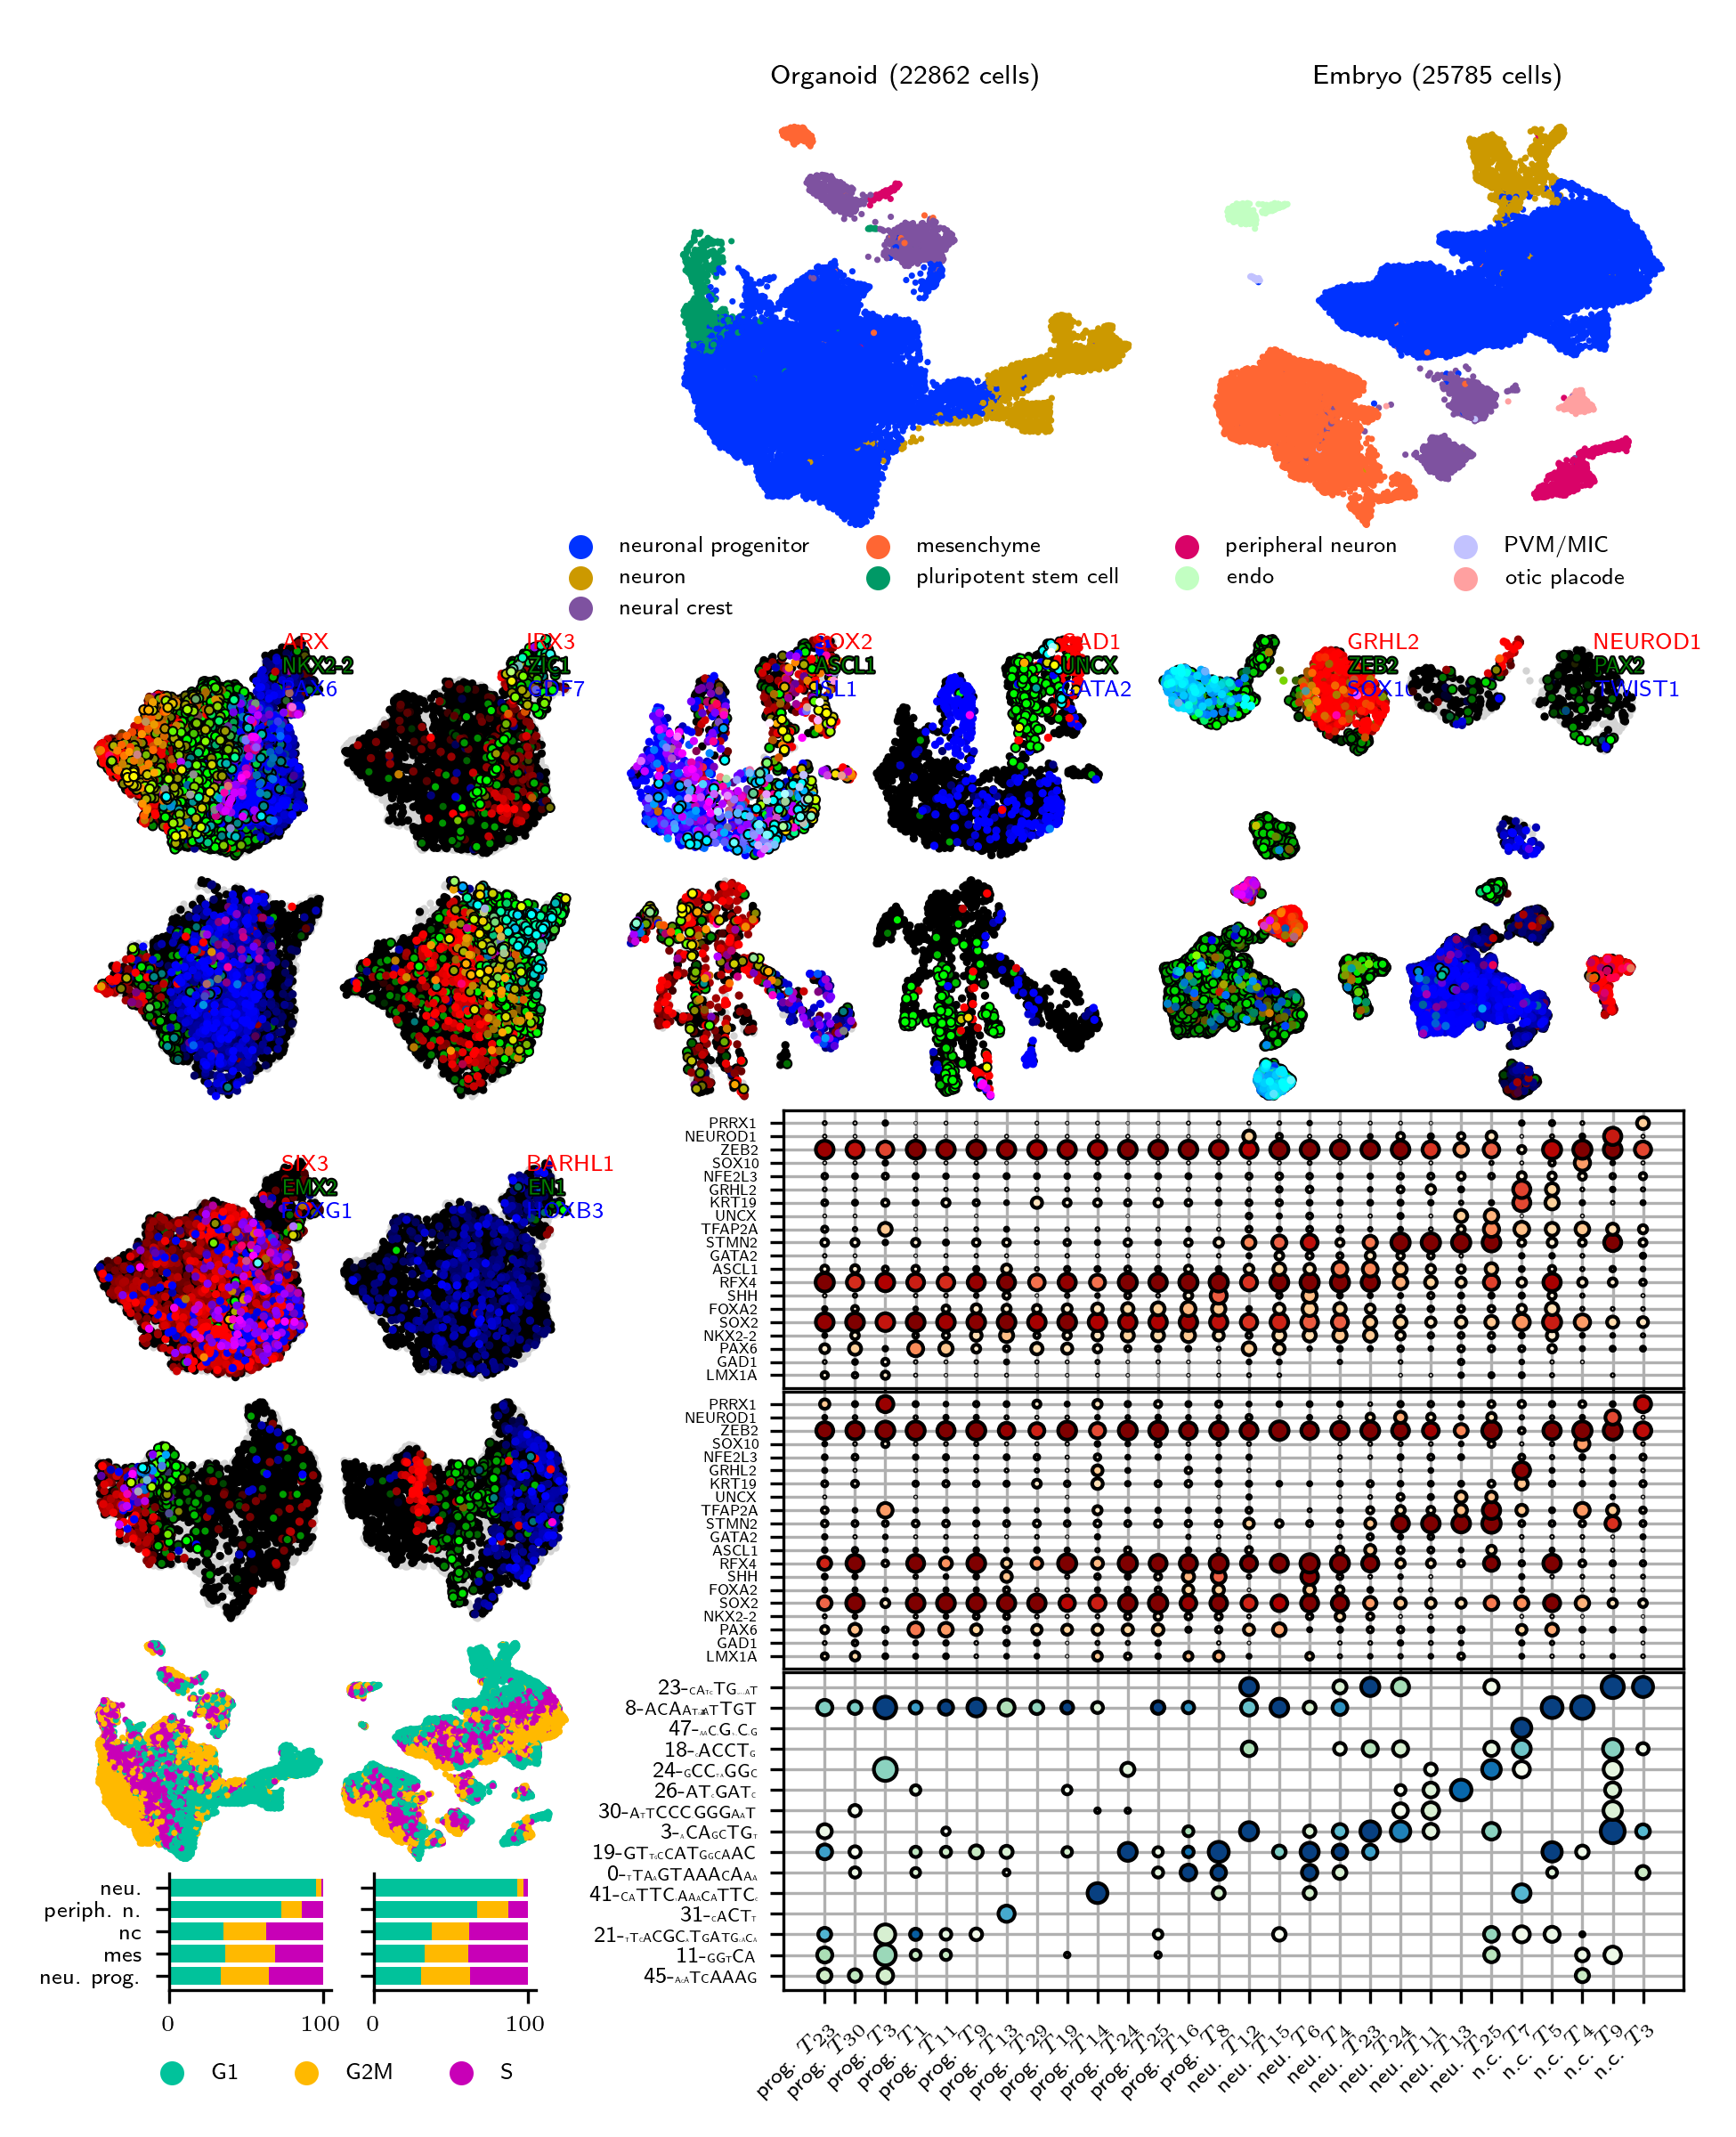
\includegraphics[width=1.0\linewidth]{figures/main/Figure_1.png}
  \caption{
    \textbf{Human neural tube organoids recapitulate early neuronal and neural crest development.} \\
    \textbf{a}, Schematic. \textbf{b-c}, UMAP based on gene expression profiles of organoid (\textbf{b}) and embryo
    (\textbf{c}) cells colored by cell type identify. \textbf{d-f}, UMAP based on gene expression profiles of organoid (top)
    and embryo (bottom) cells types showing sub-clusters of neuronal progenitors (\textbf{d}), early differentiating neurons
    (\textbf{e}) and neural crest (\textbf{f}) along with expression of indicated genes in red-green-blue color scale.
    (Continues next page)
  }
\end{figure}
\afterpage{\clearpage}

\begin{figure}[b!]
  \ContinuedFloat
  \caption*{\rule{\linewidth}{0.4pt}}
  \caption{
    (Continued) \textbf{g}, UMAP based on gene expression profiles of organoid (top; UMAP axis 1 and 2 shown) and embryo (bottom; UMAP
    axis 2 and 3 shown) for neuronal progenitor subcluster along with the expression of indicated genes in red-green-blue
    color scale. \textbf{h}, UMAP based on gene expression profiles in organoid (top left) and embryo (top right) colored by
    cell cycle phase identity and quantification of percentage of each cell for each cell cycle phase stratified by cell
    type in the organoid (bottom left) and embryo (bottom right). \textbf{i}, Average gene expression level in
    $log_{2}(CPM)$
    (dot color) and fraction of cells expressing the gene (dot size) per cell state, defined by topic modeling, for organoid
    cells (top) and embryo cells (middle) and motif enrichment level as normalized enrichment score (NES; dot color) and
    number of regions enriched for the motif (dot size) per topic (x-axis) and motif (y-axis; bottom). PVM/MIC: perivascular
    microphage/microglia.
    Color scales for RGB scatter plots are as follows (in Log(CPM)). 
    For organoid: 
    Minimum is 0 and maximum is 1.5 Log(CPM) for all genes except:
    IRX3, BAHRL1: [0, 1.0], 
    FOXG1, GAD1, UNXC, GATA2, SOX10: [0, 0.8] and 
    ZEB2 [0, 3.0], 
    For embryo: 
    Minimum is 0 and maximum is 1.5 Log(CPM) for all genes except:
    FOXG1, GAD1, UNCX, GATA2, SOX10 [0, 0.8], 
    ISL1 [0, 1.0], 
    ZEB2 [0, 3.0] and
    TWIST1 [0, 2.0].
  }
\end{figure}

\subsection*{
  DeepNeuralTube: sequence-to-function models that reveal the enhancer code underlying early neuronal and neural crest 
  development
}

In order to gain insight into the sequence characteristics underlying cell type-specific activity of neural tube-, 
neural crest- and derived cell type enhancers, we trained two sequence-to-function model convolutional neural networks:
"$DeepNeuralTube^o$" and "$DeepNeuralTube^e$". 
The models use DNA sequence of genomic regions as input and classify regions based on their cell type- or state-specific chromatin accessibility (in a multi-label multi-class fashion; \textbf(Fig. 2a)). 
The classes of the models are defined based on topic modeling. 
To get a fine-grained definition of cell states, we performed topic modeling separately for the subset of neuronal progenitors, neural crest (incl. facial mesenchyme and peripheral neurons) and early differentiating neurons for both organoid (to train $DeepNeuralTube^o$) embryo (to train $DeepNeuralTube^e$).\par

We tested the performance of $DeepNeuralTube^o$ and $DeepNeuralTube^e$ to predict cell type-specific activity 
using data from the VISTA enhancer browser\cite{viselVISTAEnhancerBrowsera2007, kosickiVISTAEnhancerBrowser2025}.
Enhancers active in the neural tube (n=349) could be classified with an area under the receiver-operator curve
(auROC) of 0.75 and 0.80 using resp. $DeepNeuralTube^o$ and $DeepNeuralTube^e$ (\textbf{Fig. 2b}; and
area under the precision-recall curve (auPR) of 0.21 resp. 0.29 (\textbf{Supplementary Fig. S2a-b})). 
Enhancers active in the facial mesenchyme (n=143) could be classified with an auROC of 0.78 and 0.79 
using resp. $DeepNeuralTube^o$ and $DeepNeuralTube^e$ (\textbf{Fig. 2c}; 
and auPR of 0.17 for both models (\textbf{Supplementary Fig. S2a-b})). 
Of note, a fraction of neural tube enhancers (24 \%) are predicted to be specific to pre-migratory neural crest by
both models. Given that the VISTA enhancers are annotated based on localization of enhancer activity only, and given
that is is difficult to visually distinguish between the neural tube and pre-migratory neural crest, this result 
is not surprising.\par

Next, we assessed the explainability of the models. Concretely we tested if the model learned known
TF binding motifs as features. To this end, we calculated pairwise similarities\cite{
  guptaQuantifyingSimilarityMotifs2007} between \textit{de novo} motifs learned by the model, 
and identified using TF-MoDISco\cite{shrikumarTechnicalNoteTranscription2018}, and known motifs that are enriched in cell type specific regions.
Clustering this pairwise similarity matrix resulted in 56 clusters (\textbf{Fig. 2d}). 
Most clusters contain known motifs enriched in regions specific to both organoid and embryo cell types (\textbf{Fig. 2e}), with the exception of cluster 13 that is organoid specific (AP1 motif; \textbf{Supplementary Table S2}) 
and cluster 26 that is embryo specific (CG-rich motif; \textbf{Supplementary Table S2}). 
More importantly, Most clusters contain at least one motif learned \textit{de novo} by the organoid and/or embryo model (\textbf{Fig. 2f-g} and \textbf{Supplementary Table S2}). 
%TODO: add percentages
Thus, $DeepNeuralTube^o$ and $DeepNeuralTube^e$ use known-motifs as features to classify regions based
on cell type-specific chromatin accessibility.\par

As an illustrative example, we investigated an enhancer located in one of the introns of \textit{GLI3} (hs111.0; \textbf{Supplementary Fig. S2c}). 
This region has neural tube specific activity in E11.5 mouse embryos (\textbf{Fig. 2h}). 
Both $DeepNeuralTube^o$ and $DeepNeuralTube^e$ explain this region similarly (Pearson correlation of x) 
%TODO: Add correlation
and highlight the importance of multiple SOX TFBS (\textbf{Fig. 2h}). 
A version of this enhancer where 5\% of the nucleotides are changed (hs111.1) does not have neural tube specific enhancer activity and both models predict that this loss of activity is due to the loss of a sinlge SOX TFBS (\textbf{Fig. 2h}).\par

Finally, to also investigate the performance of the models on migratory neural crest, 
a cell type for which there are no validated enhancers in the VISTA enhancer browser, 
we selected a genomic region that is specifically accessible in the migratory neural crest (\textbf{Supplementary Fig. S2d}). 
Both models predict this region to be specific to the migratory neural crest class (\textbf{Supplementary Fig. S2e})
and nucleotide importance scores reveal TFBS for a SOX monomer, a SOX dimer and AP2 (\textbf{Fig. 2i}). 
Next, we tested the enhancer activity of this region using an enhancer-reporter assay in chicken embryos. 
Indeed the enhancer was specifically active in migratory neural crest 24 hours after injection in an HH4 embryo (\textbf{Fig. 2i}).\par


\afterpage{\clearpage}
\begin{figure}[p]
  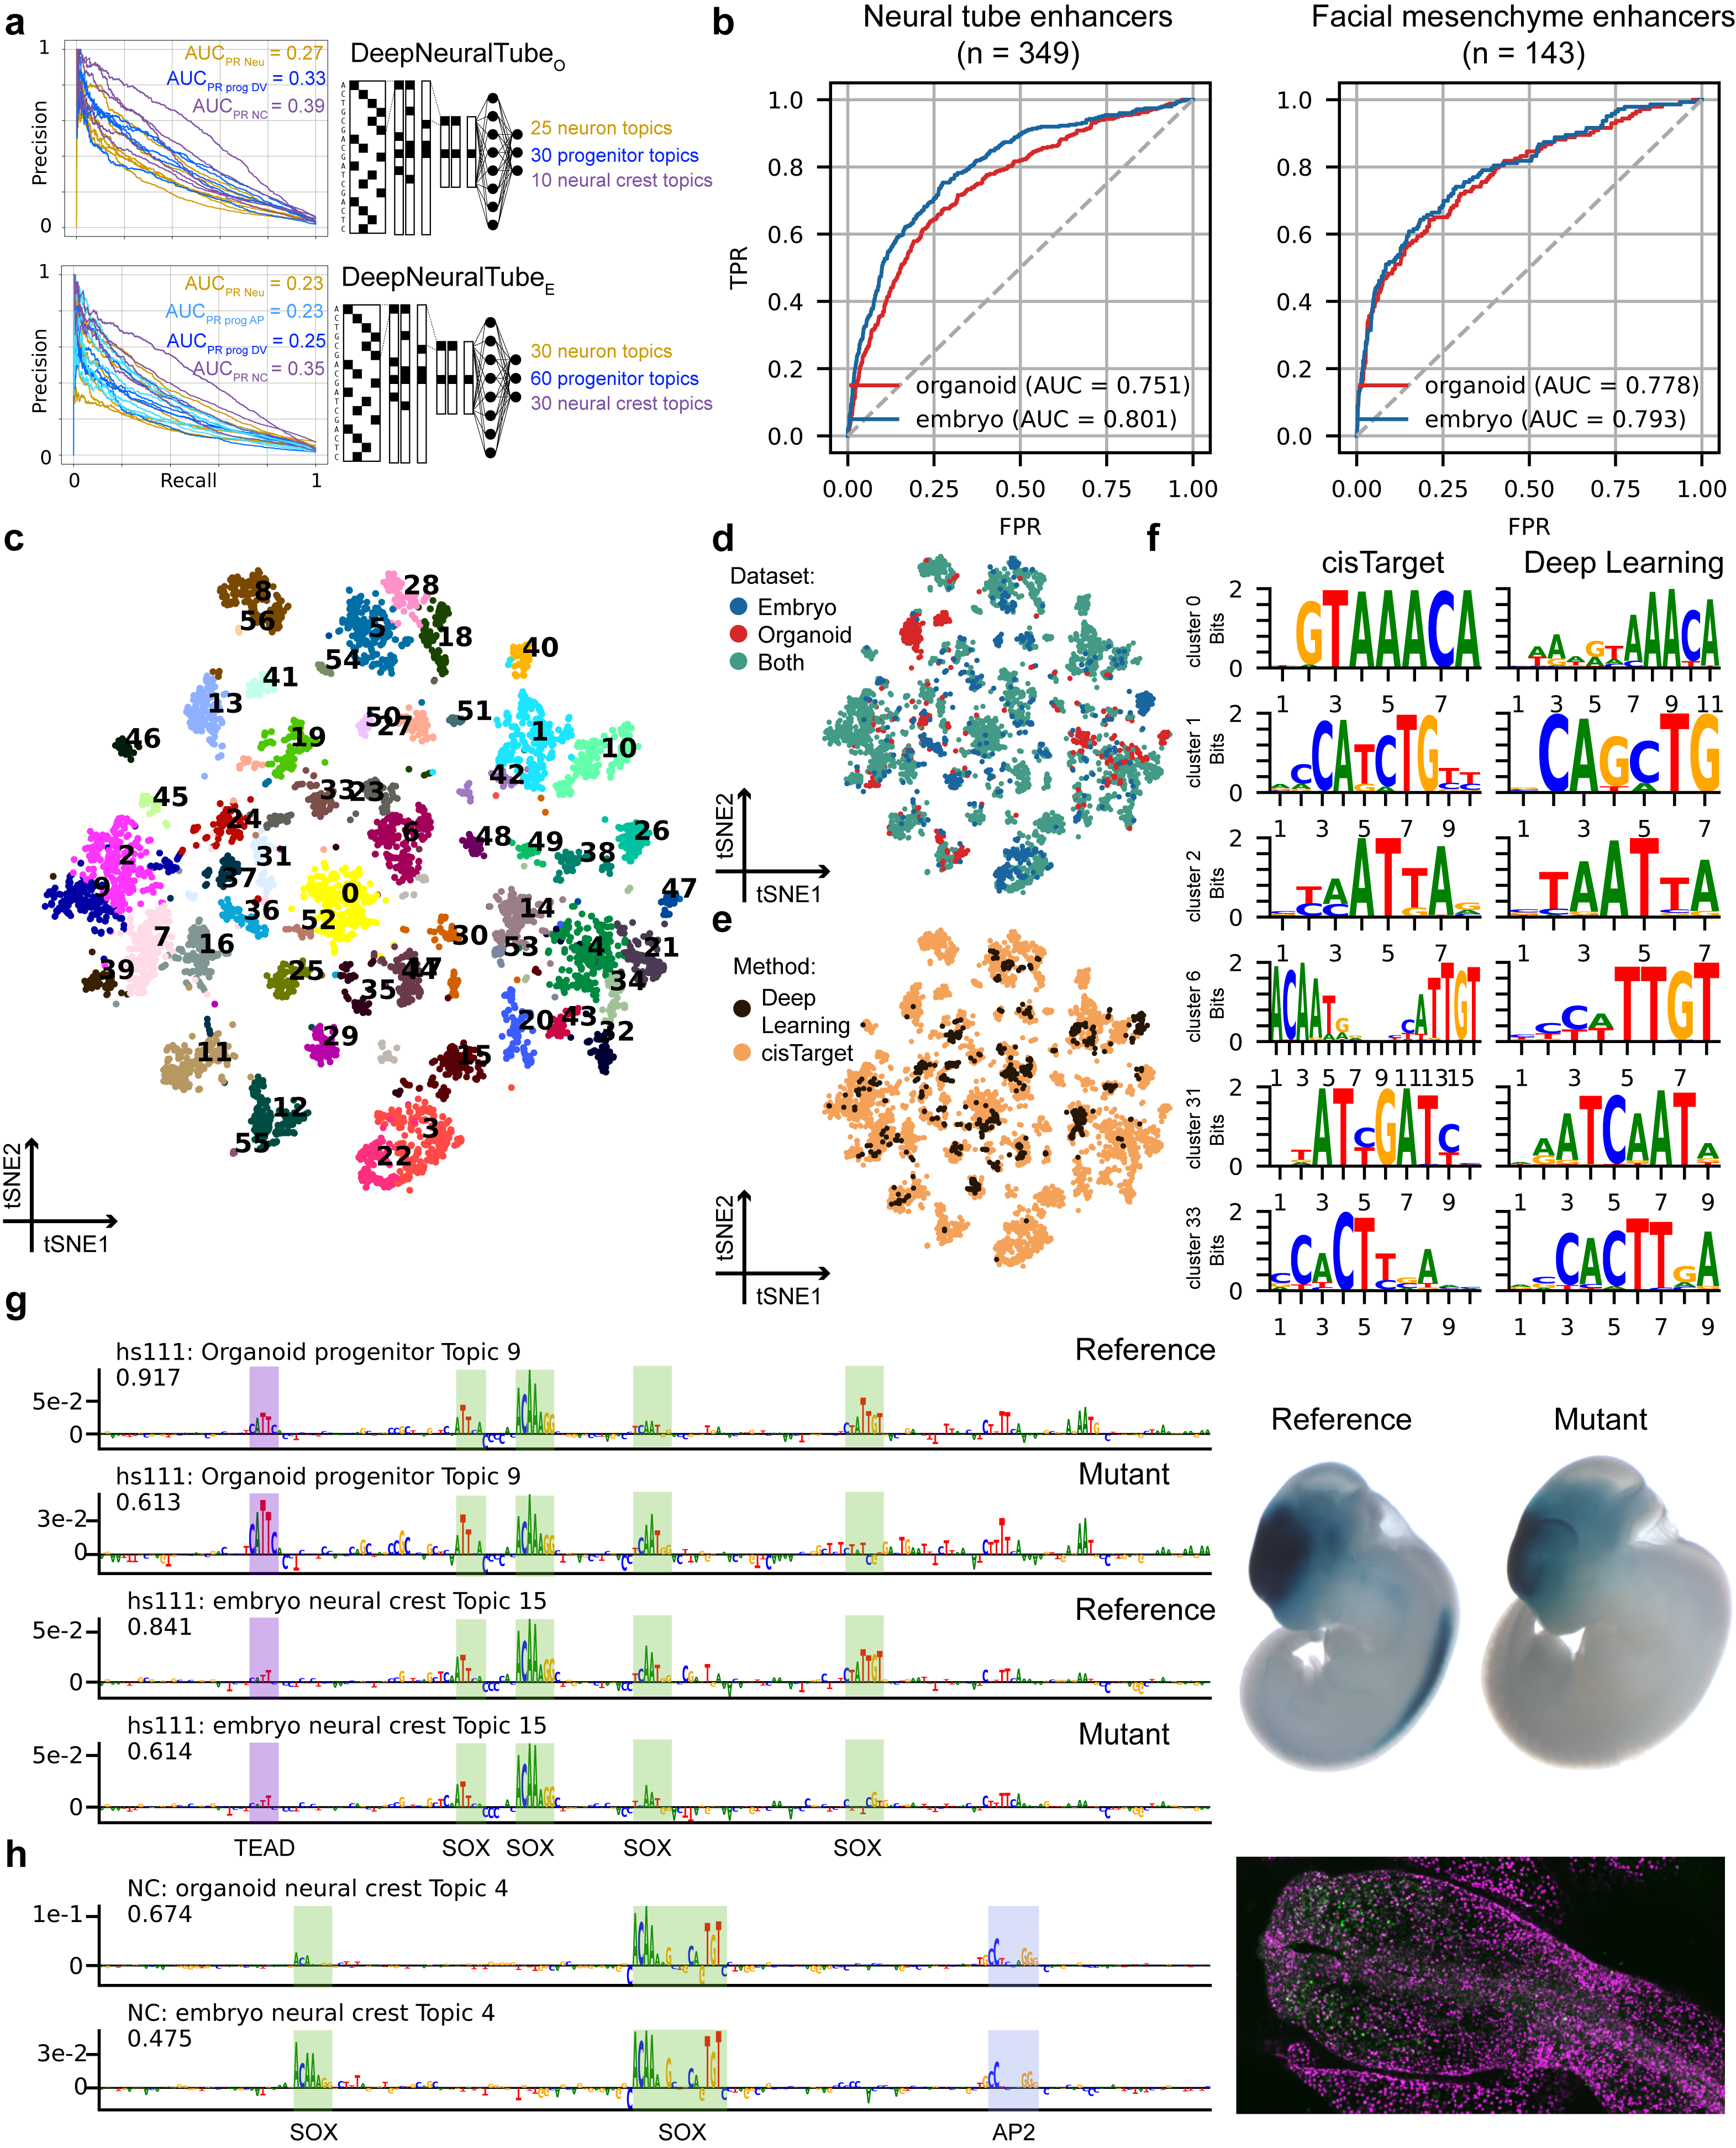
\includegraphics[width=1.0\linewidth]{figures/main/Figure_2.png}
  \caption{
    \textbf{DeepNeuralTube: an accurate sequence-to-function model revealing neuro-developmental enhancer code.} \\
    \textbf{a}, Schematic. \textbf{b} receiver-operator curves for identifying neural tube (left) and facial mesenchyme the
    $DeepNeuralTube^o$ and $DeepNeuralTube^e$. \textbf{c-e}, UMAP of TomTom [REF] motif-to-motif similarities
    using both \textit{de novo} motifs from DeepNeuralTube and known enriched motifs. Each dot is a motif. Motifs are
    colored by: cluster identity (\textbf{c}), model of origin (Continues next page)
  }
\end{figure}
\afterpage{\clearpage}

\begin{figure}[b]
  \ContinuedFloat
  \caption*{\rule{\linewidth}{0.4pt}}
  \caption{
    (Continued) (\textbf{d}; only showing \textit{de novo} motifs in this case) and whether the motif is found \textit{de novo} (Deep Learning) or by motif enrichment (cisTarget; \textbf{e}).
 \textbf{f}, Example representative motifs from clusters in b, showing motifs from motif enrichment (left) and found
    \textit{de novo} (right). \textbf{g}, contribution score for reference and mutant version of Vista enhancer hs111
    for $DeepNeuralTube^o$ (top two panels) and $DeepNeuralTube^e$ (bottom two panels) and enhancer-reporter
    assay for reference and mutant version of hs111 (right two panels) [REF]. \textbf{h}, contribution score for
    $DeepNeuralTube^o$ (top) and $DeepNeuralTube^e$ (bottom) of a genomic enhancer human neural crest
    enhancer (chr1:161200798-161201298; hg38) and enhancer-reporter assay in chicken embryo (HH4; right). Green is enhancer signal, pink is
    constitutive enhancer that serves as electroporation control.
  }
\end{figure}

\subsection*{
  The enhancer code underlying dorso-ventral patterning of neuronal progenitors
}

Focusing on neuronal progenitors, we identified topics representing cells and regions of different dorso-ventral
identities in both the organoid and the embryo data (\textbf{Fig. 3a}). 
From ventral to dorsal this is topic 36, 38, 33, 54 and 48 for the organoids and
topic 34, 38, 79, 88 and 58 for the embryo. 
As an example we first investigated two enhancers of \textit{SHH} that are strongly conserved and specific to the 
floorplate: SFPE1 and SFPE2\cite{jeongDistinctRegulatorsShh2003}. 
\textit{SHH} is most strongly expressed in the most ventral topic (33 and 34 resp. for the organoids and the embryo; \textbf{Fig. 3b}).
SFPE1 is located upstream of \textit{SHH} and SFPE2 in its second intron. Both enhancers are indeed most accessible in the cells belonging to the ventral topic (\textbf{Fig. 3c}). 
Explaining the accessibility of both enhancers using DeepNeuralTube reveals two FOX (one partial) and two RFX (one partial) binding sites in SFPE1 and two FOX, a ZEB and a TEAD binding site in SFPE2 (\textbf{Fig. 3d}).\par

To investigate the enhancer code underlying dorso-ventral patterning of neuronal progenitors further, we clustered 
and aligned \textit{de novo} motifs, identified in doros-ventral regions, based on pairwise motif similarities. 
Next, we caclulated the average contribution for all identified motif instances per cluster and for each topic 
resulting in a dorso-ventral enhancer code-table (\textbf{Fig. 3e})
Both $DeepNeuralTube^o$ and $DeepNeuralTube^e$ found similar patterns underlying the dorso-ventral states and the 
importance of the instances of these patterns is highly correlated across both models (0.75 average Pearson correlation; \textbf{Fig. 3e}). 
For the most ventral state (organoid topic 33 and embryo topic 34) a combination of FOX, TEAD and RFX instances 
are important (\textbf{Fig. 3e-f}) and the importance of these instances correlates with the expression of respectively \textit{FOXA1/A2/P2/P4}, \textit{TEAD1} and \textit{RFX3/4} in both the organoid and embryo (\textbf{Fig. 3g} and Supplementary Fig. S3). 
In subsequent more dorsal neuronal progenitor domains we observe importance of NKX instances, correlating with \textit{NKX2-1/2} expression (\textbf{(Fig. 3e- g)}); 
PAX instances, correlating with \textit{PAX3/6} expression (\textbf{Fig. 3e-g} and Supplementary Fig. S3) and 
ZIC instances, correlating with \textit{ZIC1} expression (\textbf{Fig. 3e-g} and Supplementary Fig. S3). 
For all dorso-ventral progenitor domains, except the most ventral one (and the most dorsal one in the embryo), 
SOX instances are important that correlates with the expression of\textit{SOX2/3} (\textbf{Fig. 3e-g} and Supplementary Fig. S3). 
Similarly, ZEB instances have a negative importance to the accessibility of regions in dorso-ventral domains except the most ventral one (\textbf{Fig. 3e} and Supplementary Fig. S3). 
Finally, we calculated the Jaccard index of genomic regions based on the presence of an instance of each identified pattern to investigate which patterns often co-occur in the same regions (\textbf{Fig. 3h}). 
FOX, TEAD and RFX instances often co-occur in the same genomic region while instances of other patterns tend to be present in separate regions (\textbf{Fig. 3h}).\par

It has been reported that FOXA1/2 is a pioneer factor\cite{iwafuchi-doiPioneerTranscriptionFactor2016, iwafuchiGeneNetworkTransitions2020}. 
Indeed, when centering on FOX instances we observe a strong Tn5 cute-site footprint (\textbf{Fig. 3i}). 
We then asked if there is any difference between regions that are generally bound by FOXA2 in any cell state that expresses this TF and regions, bound by FOXA2, that are specific to the floorplate. 
For this purpose, we intersected FOXA2 ChIP-seq peaks in HepG2 and A549  with floorplate peaks containing FOX instances. 
We classified the regions that overlap with any of the ChIP-seq datasets as regions that are generally bound by FOXA2 and those that did no as floorplate specific. Quantifying both the number of FOX instances per region and 
the affinity of each individual instance (making use of the FOX motif score calculated using
FIMO\cite{grantFIMOScanningOccurrences2011, schreiberTangermemeBiologicalSequence2025}) reveals that floorplate 
specific FOXA2 target regions have fewer FOX instances compared to general FOXA2 target regions (\textbf{Fig. 3j}). 
Furthermore, in case there is a single FOX instance in a general FOXA2 target region the affinity of this instance 
tends to be higher (\textbf{Fig. 3k}). These results suggest that the overall affinity of general FOXA2 target regions 
is higher (either by having a greater number of binding sites or by having binding sites with higher affinity).
Generating a \textit{de novo} motif from general and specific FOXA2 target regions that have a single FOX instance 
reveals that FOX instances in regions that are generally bound tend to be of the form \textit{TGTTT\underline{AC}} 
while those instances in specific regions tend to be of the form \textit{TGTTT} (\textbf{Fig. 3l}).\par

\afterpage{\clearpage}
\begin{figure}[p]
  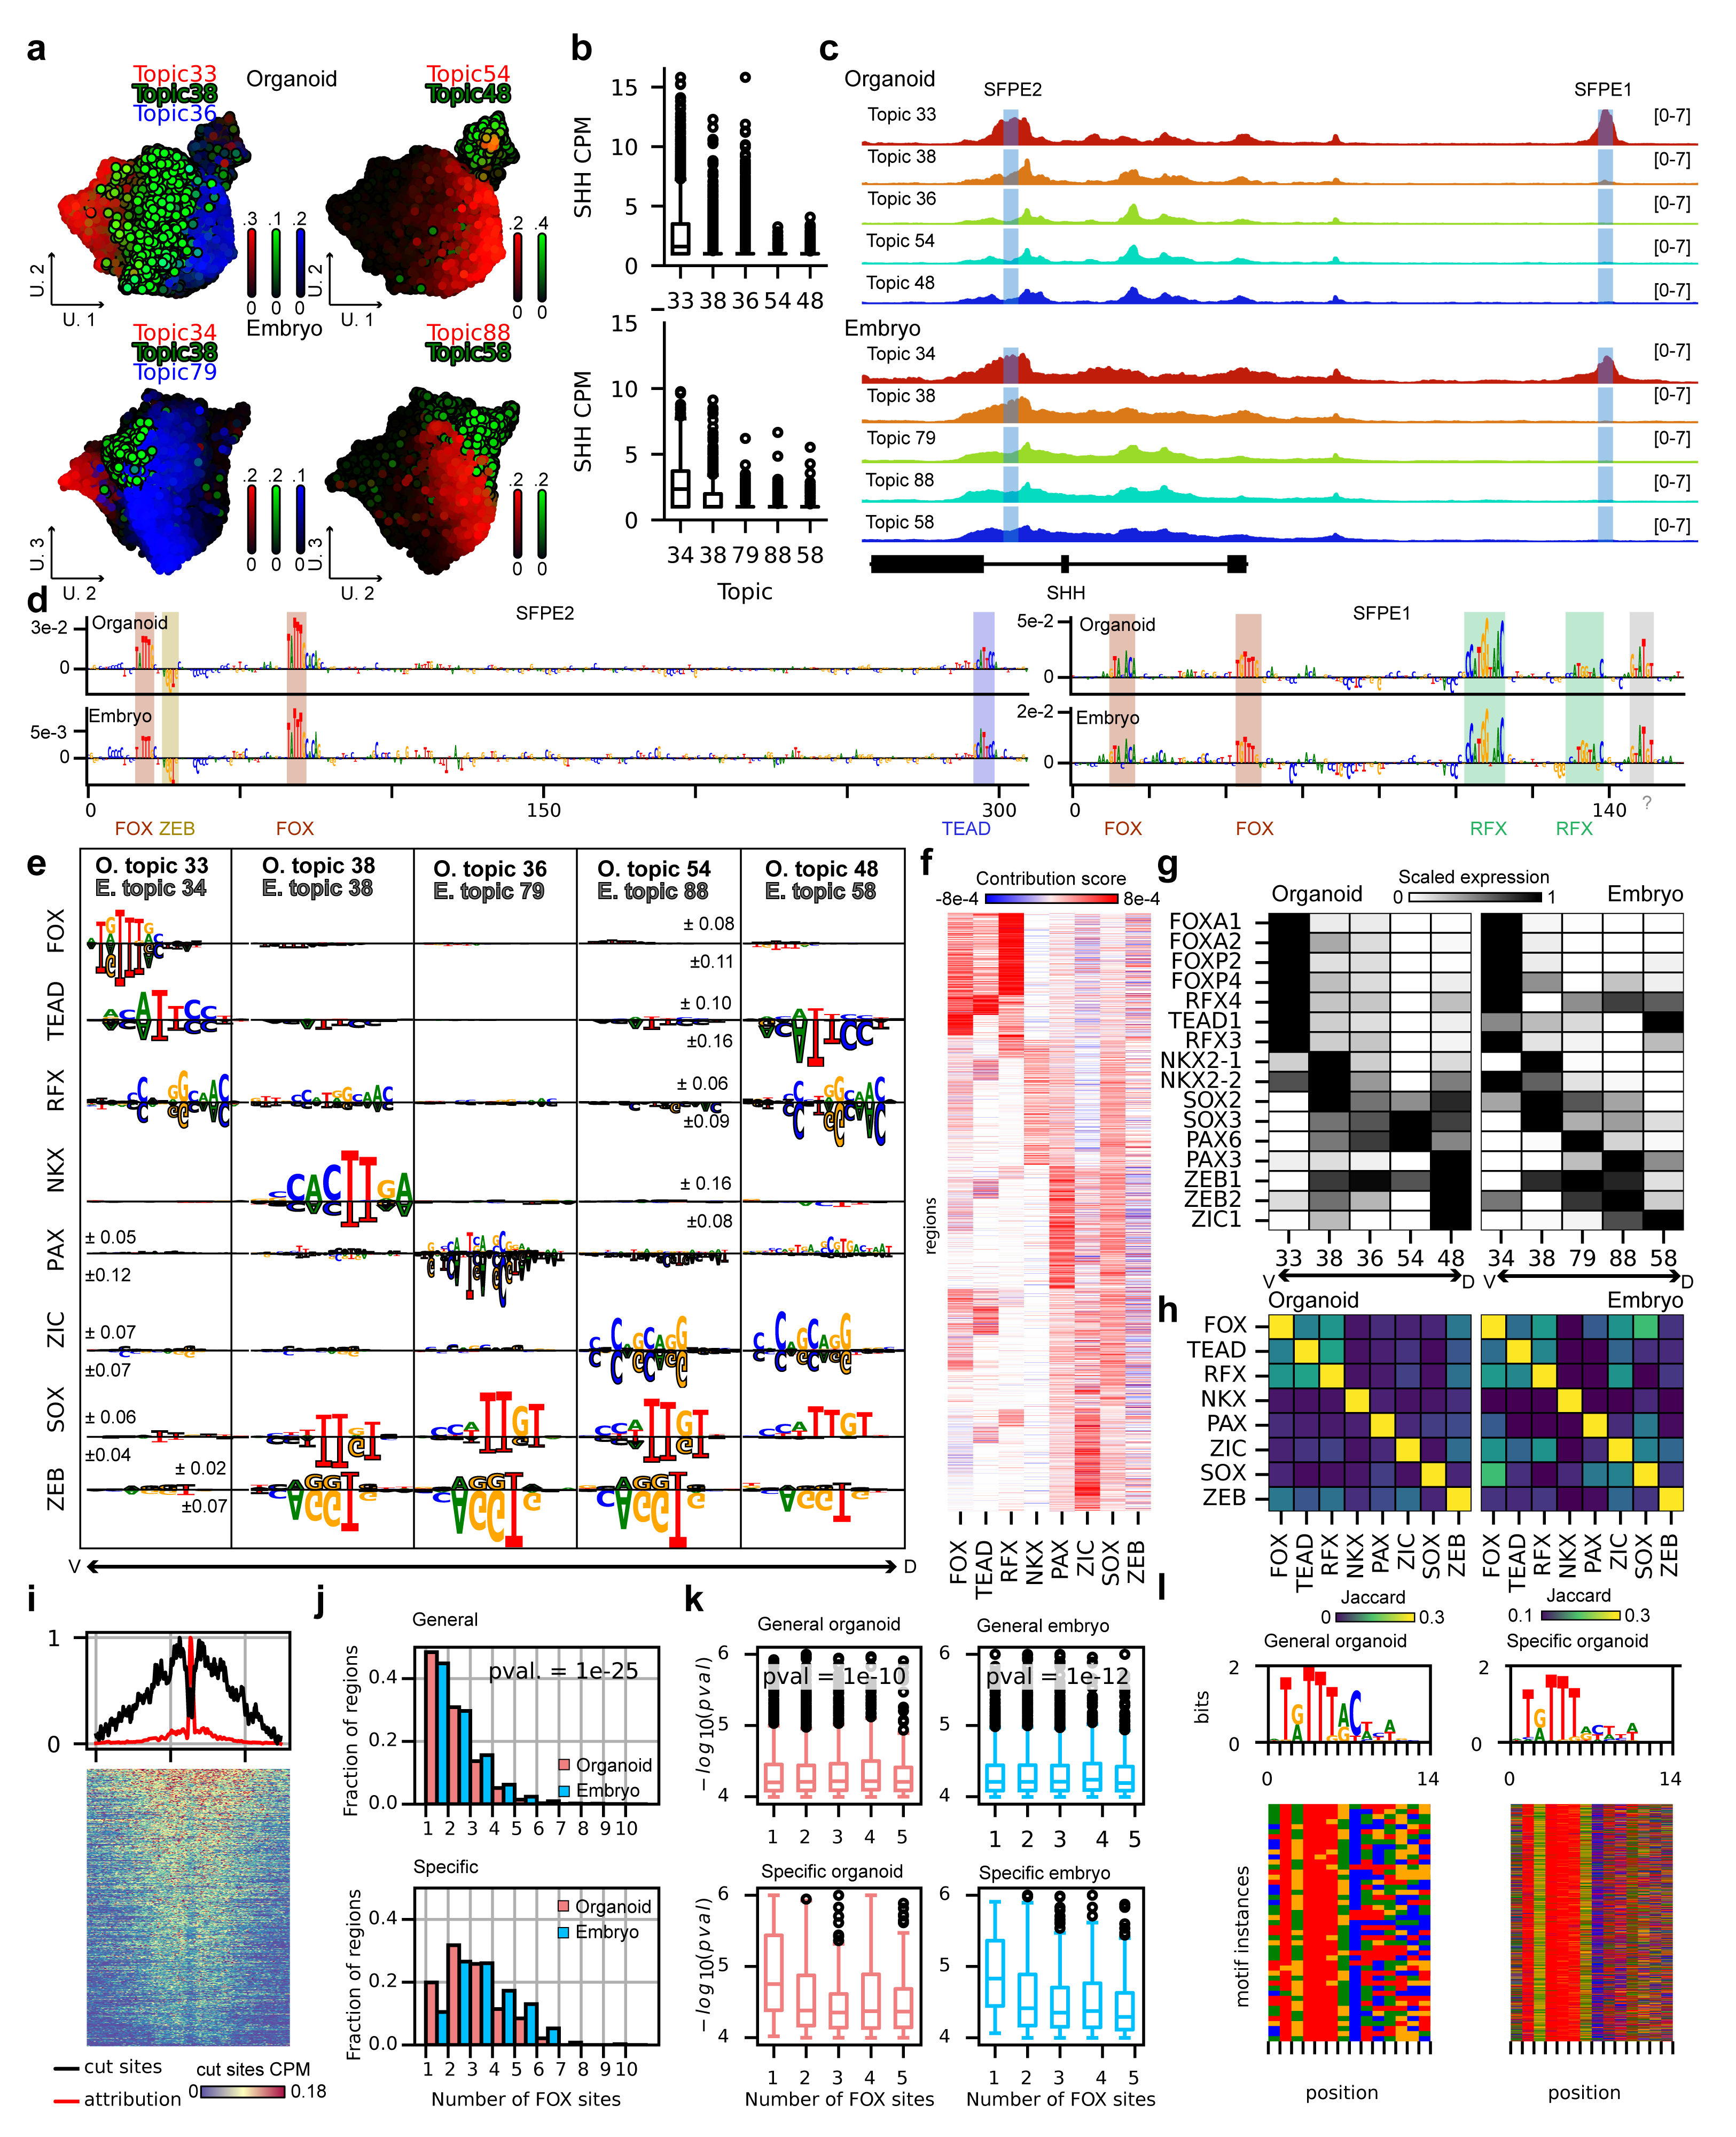
\includegraphics[width=1.0\linewidth]{figures/main/Figure_3.png}
  \caption{
    \textbf{Deciphering the enhancer code underlying dorso-ventral patterning of neuronal progenitors.} \\
    \textbf{a}, UMAP of organoid (top) and embryo (bottom) neuronal progenitors colored by cell-topic probabilities in RGB color scales of dorso-ventral topics. \textbf{b}, Boxplots of the expression of \textit{SHH} in organoid (top) and embryo (bottom) across different dorso-ventral topics ($n_{topic 33}$ = 4,571, $n_{topic 38}$ = 4,521, $n_{topic 36}$ = 6,120, $n_{topic 54}$ = 2,808, and $n_{topic 48}$ = 5,390 for organoid cells;
    and $n_{topic 34}$ = 637, $n_{topic 38}$ = 1,093, $n_{topic 79}$ = 3,939, $n_{topic 88}$ = 1,861, and $n_{topic 58}$ = 1,773 for embryo cells). (Continues next page).
  }
\end{figure}
\afterpage{\clearpage}

\begin{figure}[b!]
  \ContinuedFloat
  \caption*{\rule{\linewidth}{0.4pt}}
  \caption{
    (Continued) \textbf{c}, Chromatin accessibility in organoid (top) and embryo (bottom) across dorso-ventral topics for locus chr7:155,799,664-155,827,483 ; hg38. SFPE2 and SFPE1 is highlighted. \textbf{d}, Nucleotide contribution scores for SFPE2 (left) and SFPE1 (right) for organoid topic 33 (top) and embryo topic 34 (bottom). \textbf{e}, Code table showing average contribution score of pattern instances for each dorso-ventral topic. Contribution scores for $DeepNeuralTube^o$ are not outlined. Contribution scores for $DeepNeuralTube^e$ are outlined and negated. \textbf{f}, Heatmap showing the maximum normalized contribution score for each of the top 1,000 regions per topic (y-axis) and pattern (x-axis) for dorso-ventral topics. \textbf{g}, Heatmap showing scaled expression of transcription factors corresponding to identified patterns in organoid (left) and embryo (right) dorso-ventral topics. \textbf{h}, Heatmap showing Jaccard index of regions based on the presence of instances of the identified patterns. \textbf{i}, Scaled average and normalized number of cut sites (black, top) and contribution score (red, top) across genomic regions with a FOXA2 instance and heatmap showing normalized number of cut sites (bottom) for individual regions with a FOXA2 instance. Signal is centered on the FOXA2 instance start position. \textbf{j}, Bar chart showing the fraction of genomic regions that has a given number of FOXA2 instances for FOXA2 regions that overlap with HepG2 or A549 FOXA2 ChIp-seq signal (general; bottom) and those regions that don't overlap (specific; top). \textbf{k}, Boxplot (ADD NUMEBRS) showing $-log_10(p value)$ of FOXA2 motif hits calculated using FIMO\cite{grantFIMOScanningOccurrences2011,schreiberTangermemeBiologicalSequence2025} for general regions (bottom) and specific regions (top) stratified by the number of FOXA2 instance per region. \textbf{l}, \textit{de novo} motif for regions with a single FOXA2 instance that are specific (left, top) or general (right, top) and heatmap color coded by nucleotide identity for individual regions for both specific (left, bottom) and general (right, bottom) regions that have a single FOXA2 instance.
  }
\end{figure}


\subsection*{
  Anterior-posterior patterning in neuronal progenitors is regulated by different homeodomain transcription factors that each recognize a distinct binding site.
}

In the embryo we observed neuronal progenitors states of different anterior-posterior (AP) identities (\textbf{Fig. 1g}).
We identified seven topics corresponding to different AP domains, from anterior to posterior this is Topic 61, Topic 59, Topic 31, Topic 62, Topic 70, Topic 52 and Topic 71 (\textbf{Fig. 4a}). 
We first asked if the AP-program is distinct from the DV program. 
In other words, is AP patterning encoded in the same or in different genomic regions as DV patterning? 
For this purpose, we calculated the pairwise correlation between region-topic probabilities of all AP and DV topics (\textbf{Fig. 4b}). 
This revealed that both AP and DV patterning are mostly encoded in distinct genomic regions, 
with the exception of AP Topic 59 and 31 that correlate with the region-topic probability of DV Topic 38 
(which corresponds to cells expressing \textit{NKX2-1/2}; \textbf{Fig. 4b})\par

$DeepNeuralTube^e$ was able to distinguish the different AP domains but grouped topics of similar domains
together (i.e., Topic 59, 31 and 62; Topic 52 and 71), resulting in four distinct AP domains (\textbf{Fig.4 c-d}). 
By explaining the predictions of $DeepNeuralTube^e$ on the regions of those domains we found four distinct
homeodomain TF binding motifs, one for each domain (\textbf{Fig. 4e}). 
From anterior to posterior this is \textit{TAATTA}, \textit{GGATTA}, \textit{TCATGWTGANTGA} and \textit{CATYMATCA}.
Notably, the patterns corresponding to the two posterior most topics correspond to dimer-motifs. 
Previously it was already hypothesized that genome-wide specific binding of homeodomain TFs is accomplished through
cooperative binding of two TFs\cite{mannChapter3Hox2009}. 
Indeed, the presence of instances of the \textit{TCATGWTGANTGA} motif correlates with the expression of both \textit{PAX5/8} and \textit{EN1/2} 
and the prescence of instances of the \textit{CATYMATCA} motif correlates with the expression of \textit{MEIS1/2}, \textit{PBX1/2} and \textit{HOXB3} (\textbf{Fig. 4d-e} and Supplementary Fig. S4). 
In contrast, the patterns corresponding to the two anterior most topics correspond to monomer motifs, 
correlating with the expression of \textit{LHX2/9}, \textit{RAX} and \textit{SIX3/6} for the most anterior topic and 
with the expression of \textit{OTX1/2}, \textit{EMX2}, \textit{DMBX1} and \textit{LMX1A} for the second most anterior
topic (\textbf{Fig. 4d-e} and Supplementary Fig. S4)\par
%TODO: I'm surprised to see EMX2 (forebrain) together with OTX1/2 and DMBX1 (midbrain)

Focusing on the two most anterior domains, two similar homeodomain TF binding motifs seem to underlie the differential
accessibility of those domains. Both have the core homeobox motif "\textit{TAAT}" 
but one is flanked by the nucleotides \textit{TAG} while the other is flanked by the nucleotides \textit{CCCT}. 
%TODO: Do we know which TFs these correspond to? If you do, mention it in the text
We were surprised that this slight difference in the two motifs would be enough for encoding two separate AP domains.
To test this hypothesis, we first did a substitution experiment where we replaced all instances of
\textit{CTAAT\underline{TAG}} with \textit{CTAAT\underline{CCCT}} in regions of the most anterior domain and vice
versa (\textbf{Fig. 4f}). 
Indeed, $DeepNeuralTube^e$ predicts an anterior-to-posterior shift of accessibility of those regions after the \textit{CTAAT\underline{TAG}} to \textit{CTAAT\underline{CCCT}} substitution and 
vice versa a posterior-to-anterior shift of accessibility after the \textit{CTAAT\underline{CCCT}} to
\textit{CTAAT\underline{TAG}} substitution (\textbf{Fig. 4f}). 
Next, we designed enhancers from scratch by embedding either the \textit{CTAAT\underline{TAG}} or 
\textit{CTAAT\underline{CCCT}} motif\cite{taskiranCelltypedirectedDesignSynthetic2024, kempynckCREstedModelingGenomic2025} 
and using respectively Topic 61 and Topic 31 as target class (\textbf{Fig. 4g}). 
Embedding of two instances of either motif was sufficient to reach predicted chromatin accessibility levels of equivalent ranges to the predicted chromatin accessibility levels of genomic regions (\textbf{Fig. 4g}). 
Next, to eliminate potential model bias we repeated the same experiment but optimized for the opposite class. 
This is, we optimized for Topic 31 by embedding the \textit{CTAAT\underline{TAG}} motif and we optimized for Topic 61
by embedding the \textit{CTAAT\underline{CCCT}} motif (\textbf{Fig. 4h}). 
In this case, the synthetic design failed to converge for the target class but instead regions with high prediction 
score for the AP domain that corresponds to the motif used for embedding were generated. 
This is embedding of the \textit{CTAAT\underline{TAG}} motif still generated regions with high prediction score for Topic 61 
and embedding of the \textit{CTAAT\underline{CCCT}} motif generated regions with high prediction score for Topic 31 (\textbf{Fig. 4h}), even though the prediction score was optimized towards the opposite class\par

These results suggest that an unsophisticated code using two distinct motifs is sufficient to distinguish between the two utmost neuronal progenitor AP domains. 
Encouraged by this finding, we trained a logistic regression model to classify genomic regions of those two domains 
in either Topic 61 or Topic 31 using as features only the motif scores of the two motifs identified above (\textbf{Fig. 4i}). 
Surprisingly, this very simple classifier reached high performance with area under the ROC of 0.82 and area under the precision recall curve of 0.80 (\textbf{Fig. 4i}).\par

\afterpage{\clearpage}
\begin{figure}[p]
  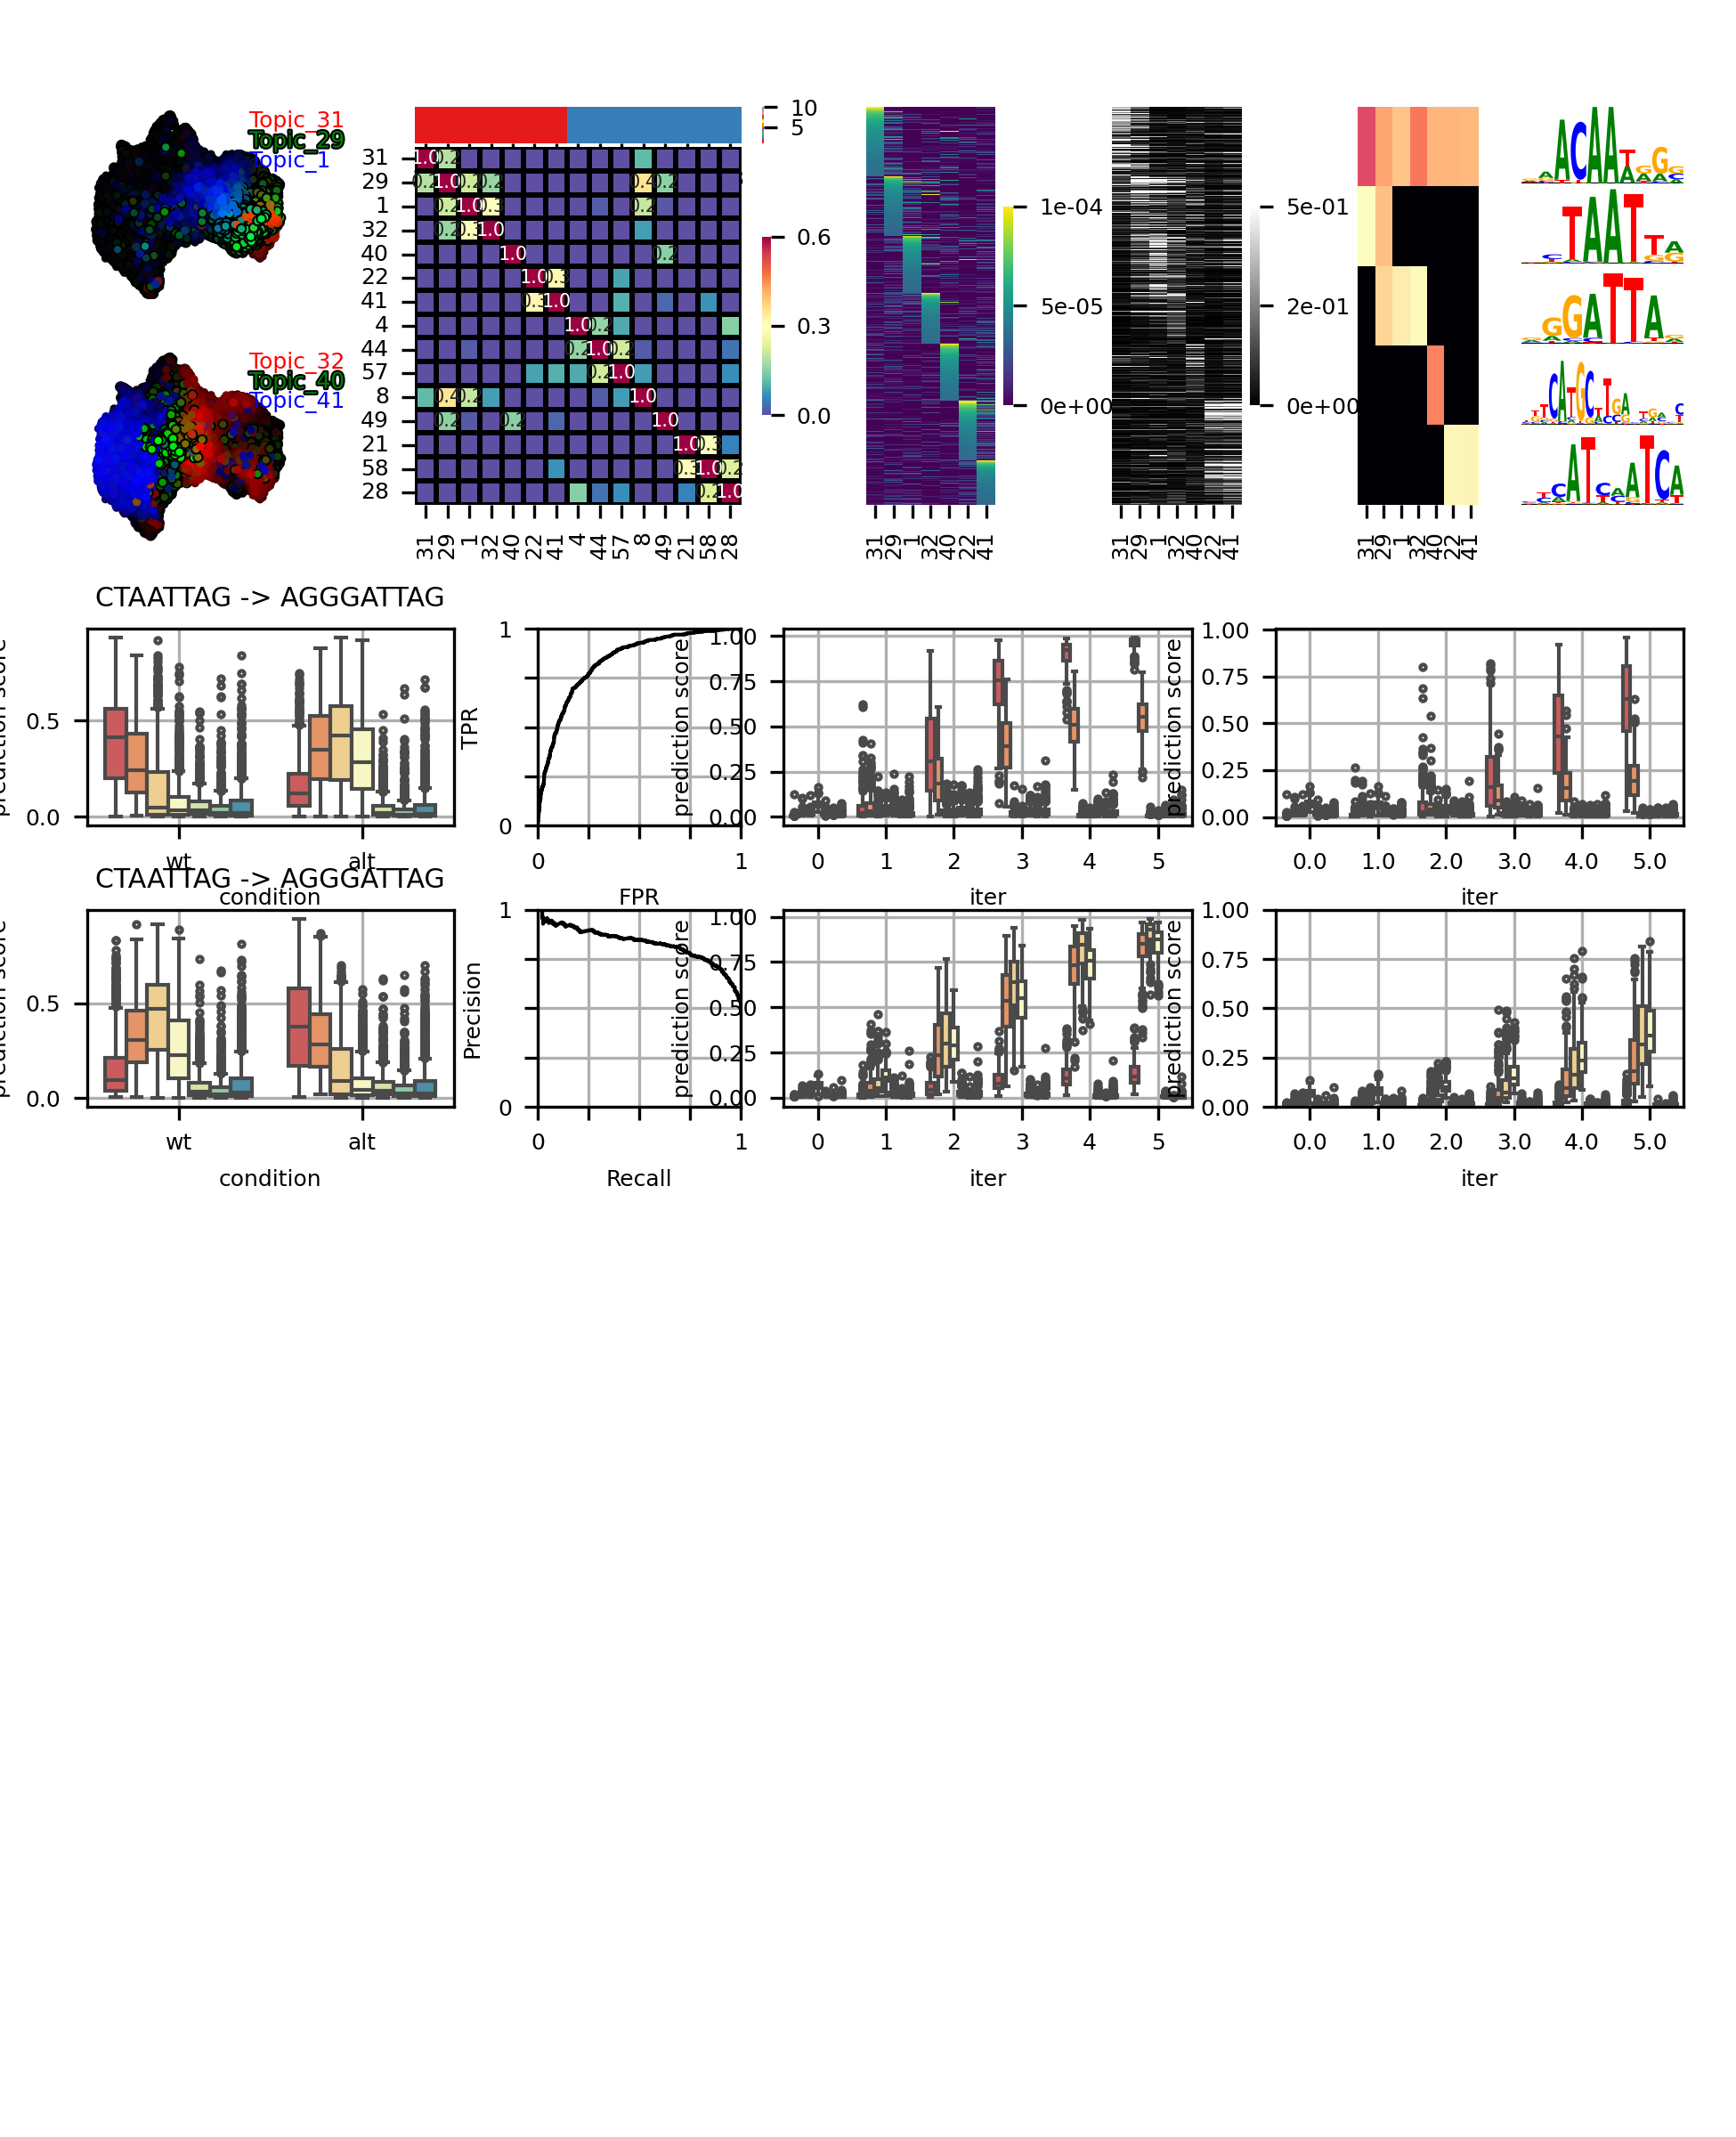
\includegraphics[width=1.0\linewidth]{figures/main/Figure_4.png}
  \caption{
    \textbf{A simple enhancer code underlies anterior-posterior patterning in neuronal progenitors.} \\
  \textbf{a}, UMAP of embryo neuronal progenitors colored by cell-topic probabilities in RGB color scales for
anterior-posterior topics. \textbf{b}, Heatmap showing pairwise pearson correlation coefficients of region-topic probabilities for dorso-ventral and anterior-posterior topics. \textbf{c}, Heatmap showing region-topic probabilities for the top 3,000 regions per topic (y-axis) and each anterior-posterior topic (x-axis). \textbf{d}, Heatmap showing prediction scores of $DeepNeuralTube^e$ on the topic 3,000 regions per topic (y-axis) for each anterior-posterior topics (x-axis).\textbf{e}, Heatmap showing the log of the number of seqlets for each identified pattern (y-axis) for all anterior-posterior topics (x-axis).\textbf{f}, Boxplot showing prediction score before (wt) and after (alt) substituting all instances of \textit{CTAATTAG} with \textit{CTAATCCCT} (top) or substituting all instances of \textit{CTAATCCCT} with \textit{CTAATTAG} (bottom) in the topic 3,000 regions of either Topic 61 or Topic 31. \textbf{g}, Boxplot showing prediction scores for all anterior-posterior topics after embedding 0 to 5 instances of \textit{CTAATTAG} while optimizing their location for Topic 61 (top) and after embedding 0 to 5 instances of \textit{CTAATCCCT} while optimzing their location for Topic 31 (bottom); n = 200. \textbf{h}, Boxplot showing prediction scores for all anterior-posterior topics after embedding 0 to 5 instances of \textit{CTAATTAG} while optimizing their location for Topic 31 (top) and after embedding 0 to 5 instances of \textit{CTAATCCCT} while optimzing their location for Topic 61 (bottom); n = 200. .\textbf{i}, receiver-operator curve (ROC) (top) and precision-recall curve (bottom) for logistic regression classifier classifying genomic regions as either Topic 61 or Topic 31 based on motif scores for \textit{CTAATTAG} and \textit{CTAATCCCT} motifs.
  }
\end{figure}
\afterpage{\clearpage}

\newpage

\subsection*{
  The enhancer code underlying pre-migratory and migratory neural crest and facial mesenchyme.
}

Focusing on neural crest cells, we identified topics representing cells and regions of both pre- and migratory neural
crest as well as facial mesenchyme (\textbf{Fig. 5a}). Similar to the neuronal progenitors, we used
$DeepNeuralTube_{oranoid}$ and $DeepNeuralTube^e$ to generate a neural crest code-table (\textbf{Fig. 5b}). 
Again, both $DeepNeuralTube^o$ and $DeepNeuralTube^e$ found similar patterns and the importance of the instances of
these patterns is highly correlated across both models (0.73 average Pearson correlation coefficient; \textbf{Fig. 5b}).\par

Organoid Topic 62 and embryo Topic 103 represent the pre-migratory neural crest state and 
instances of TEAD, GRHL, AP2 and ZEB patterns are important for this state (\textbf{Fig. 5b-c}) 
the importance of TEAD instances correlates with \textit{TEAD3/4} expression, 
GRHL with \textit{GRHL1/1} 
and AP2 with both \textit{TFAP2A} and \textit{TFAP2C} (\textbf{Fig. 5d} and Supplementary Fig. S5). 
Note that ZEB instances have a positive contribution to the pre-migratory while it has a 
negative contribution to all other neural crest states (\textbf{Fig. 5b-c}); 
and moreover a negative contribution to all other cell states of both the neuronal progenitors (\textbf{Fig. 3e}) and neurons (\textbf{Fig. 6b}). 
The positive contribution of ZEB in the pre-migratory neural crest state coincides with the absence of the expression of both \textit{ZEB1} and \textit{ZEB2} (\textbf{Fig. 5d} and Supplementary Fig. S5). 
This is in line with the previously reported role of ZEB2 as a chromatin closing repressor \cite{taskiranCelltypedirectedDesignSynthetic2024}.\par

The migratory neural crest cell state is represented by two organoid topics (Topic 65 and 59) and a single embryo topic (Topic 94). 
Nuclear receptor, AP2, ZIC (only in organoid topics) and SOX-dimer (organoid Topic 59 but not 65) are important for this state (\textbf{Fig. 5b-c}). 
We could not link the nuclear receptor instances to a specific TF based on the correlation of expression and the importance score of these instances. 
The importance of AP2 instances correlates with the expression of \textit{TFAP2A}, \textit{TFAP2B} and \textit{TFAP2C} (\textbf{Fig. 5d}), 
ZIC with \textit{ZIC1} to \textit{ZIC5} and 
the SOX-dimer with expression of \textit{SOX10} (\textbf{Fig. 5d} and Supplementary Fig. S5). 
The switch from TFAP2A/C in pre-migratory neural crest to TFAP2A/B in migratory neural crest is consistent with a previously reported function of both heterodimers in respectively neural plate border induction and neural crest specification\cite{rothsteinHeterodimerizationTFAP2Pioneer2020}. 
After the pre-migratory and before the migratory neural crest state another topic is found in both organoid (Topic 60) and embryo (Topic 105) 
for which instances of RFX are important (\textbf{Fig. 5b-c}) correlating with the expression of \textit{RFX3/4} (\textbf{Fig. 5d} and Supplementary Fig. S5).\par

Finally, the facial mesenchyme cell state is represented by organoid Topic 58 and embryo Topic 91. 
Instances of a FOX patterns and a dimer consisting of a homeobox and ebox motif are important for this state (\textbf{Fig. 5b}). 
The importance of the FOX instances correlates with the expression of \textit{FOXC2/D1/P1/P2} and 
that of the dimer motif with the expression of both \textit{TWIST1} and \textit{ALX1/4} and \textit{PRRX1} (\textbf{Fig. 5d} and Supplementary Fig. S5). 
The latter is consistent with a recent study where it has been shown that TWIST1 and homeodomain TFs cooperatively
bind this specific dimer motif regulating the expression of genes involved in
facial mesenchyme\cite{kimDNAguidedTranscriptionFactor2024}.\par

Next, we investigated which patterns co-occur in the same genomic regions. For this purpose, we calculated the Jaccard
index of genomic regions based on the presence of an instance of each identified pattern (\textbf{Fig. 5e}). Using this
method we found three sets of regions that are predicted to contain instances of different set of TFs. One set where
instances of TEAD, GRHL and ZEB co-occur, one where instances of Nuclear receptor, AP2 and ZIC
instances co-occur, and one set where instances of FOX and TWIST1/homeodomain co-occur.\par
%TODO: C.M.: Mesenchyme+NC or calculated over all regions?

Recently, a genome wide association study (GWAS) identified 203 single-nucleotide polymorphisms (SNPs)
that are associated with facial variation\cite{whiteInsightsGeneticArchitecture2021}. 
Given that regions surrounding these SNPs were enriched for enhancer activity in cranial neural crest cells\cite{whiteInsightsGeneticArchitecture2021} 
we asked if, using $DeepNeuralTube$, we could explain the effect of some of these variants on enhancer activity. Therefore for all suggestive SNPs we scored both the reference and alternative allele(s) using both $DeepNeuralTube^o$ and $DeepNeuralTube^e$ 
and calculated the difference in prediction score across both alleles (delta prediction score). 
At an absolute delta prediction score threshold of 0.2 we identified 235 SNPs that are explainable by either of the two models. 
Note that only very few (1 out of 203) of these "explainable" SNPs overlap with the 203 lead SNPs identified by White \textit{et al.} (\textbf{Fig. 5f}). 
Most of the "explainable" SNPs have a high delta prediction score for either organoid neural crest Topic 58 or Topic 59 (\textbf{Supplementary Fig. S6}). 
As an example we show the explanation of rs1555067 that is located upstream of \textit{PRRX1}. 
The G \textgreater A substitution of this SNP causes a delta prediction score of 0.64 for organoid Topic 58
(\textbf{Fig. 5g}), increasing the predicted chromatin accessibility of this genomic region in the facial mesenchyme. 
This predicted increase in chromatin accessibility is caused by generating an EBOX site 6bp downstream of a partial
homeobox site potentially creating a new binding site for TWIST1-homeodomain TF dimers (\textbf{Fig. 5h}).\par


\afterpage{\clearpage}
\begin{figure}[p]
  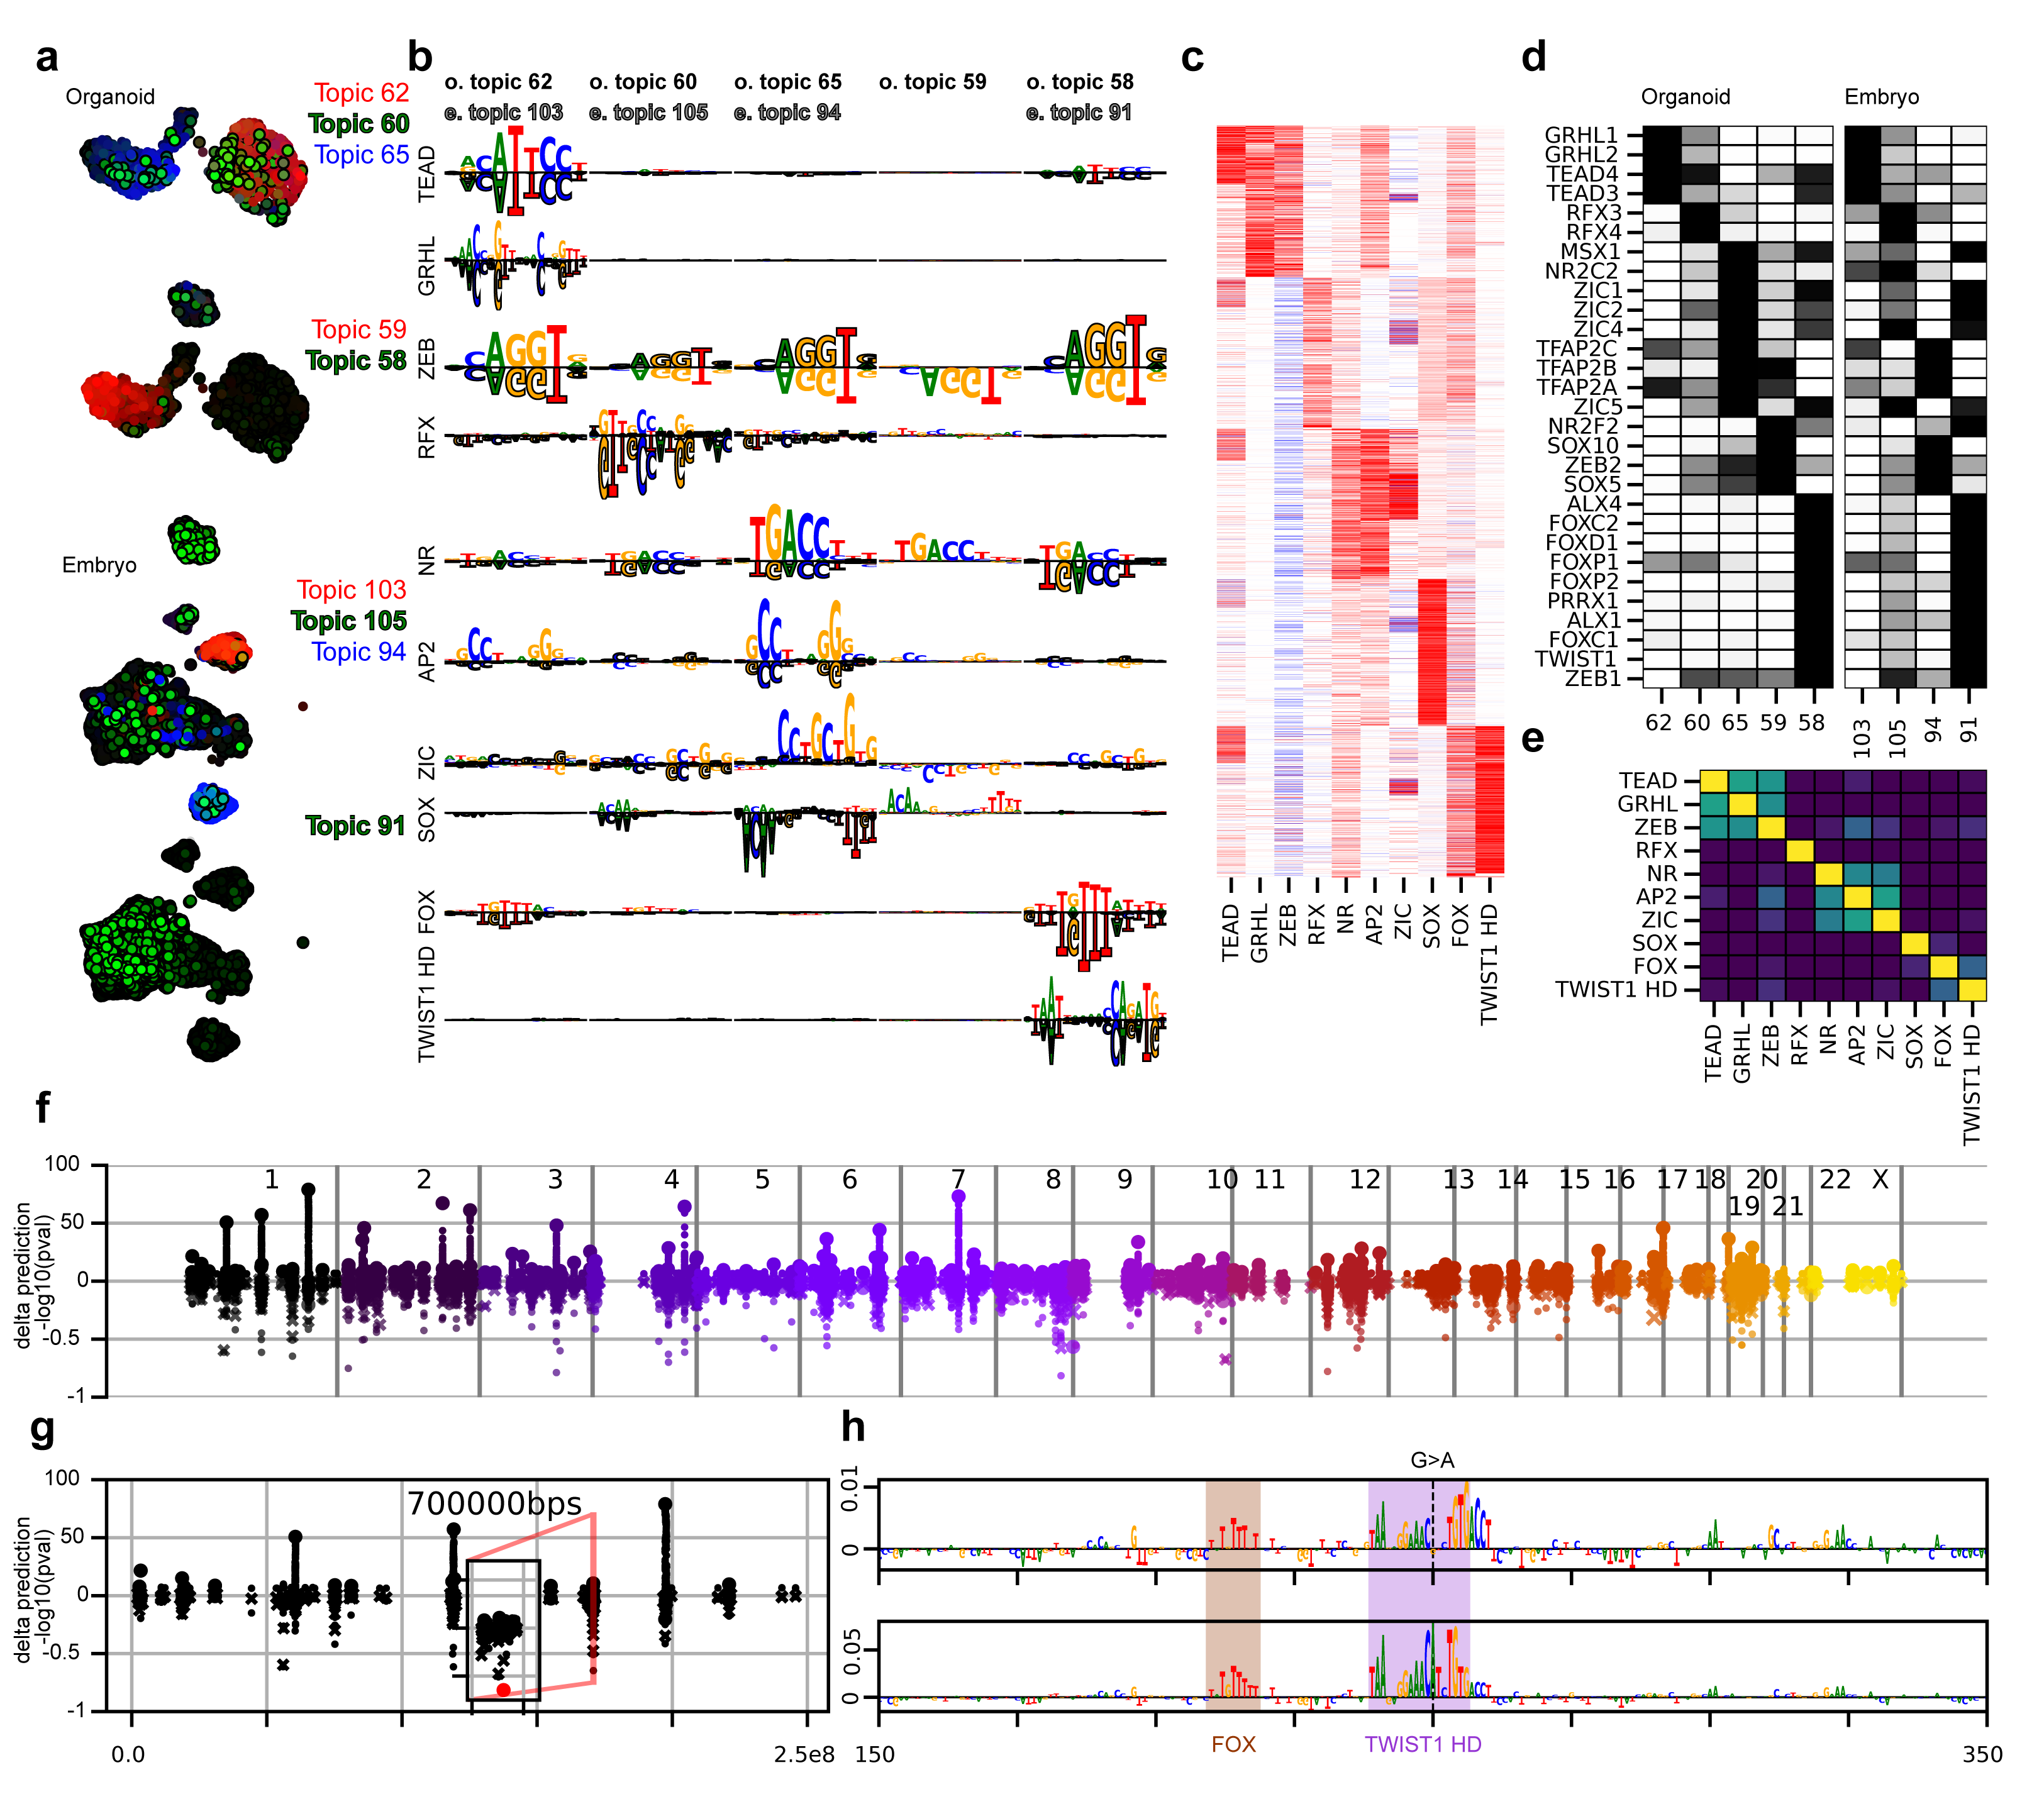
\includegraphics[width=1.0\linewidth]{figures/main/Figure_5.png}
  \caption{
    \textbf{Deciphering the enhancer code underlying pre-migratory and migratory neural crest and facial mesenchyme.} \\
\textbf{a}, UMAP of organoid (top two) and embryo (bottom two) neural crest cells colored by cell-topic probabilities in RGB color scales for neural crest related topics. \textbf{b}, Code table showing average contribution score of pattern instances for each neural crest related topic. Contribution scores for $DeepNeuralTube^o$ are not outlined. Contribution scores for $DeepNeuralTube^e$ are outlined and negated. \textbf{c}, Heatmap showing the maximum normalized contribution score for each of the top 1,000 regions per topic (y-axis) and pattern (x-axis) of neural crest related topics. \textbf{d}, Heatmap showing scaled expression of transcription factors corresponding to identified patterns in organoid (left) and embryo (right) for neural crest related topics. \textbf{e}, Heatmap showing Jaccard index of regions based on the presence of instances of the identified patterns. \textbf{f}, Manhattan plot showing -log p value of the SNP being associated with variations in facial shape\cite{whiteInsightsGeneticArchitecture2021} (positive y-axis) and the maximum (across classes of the model) of the absolute value of the difference in prediction score between the reference and alternative allele (negative y-axis; circles for $DeepNeuralTube^o$ and crosses for $DeepNeuralTube^e$) across the human genome. Lead SNPs are shown with a bigger dot size. \textbf{g}, Zoom in of chromosome one with the locus of SNP rs1555067 shown as an inset, the SNP itself is shown in red. \textbf{h}, Nucleotide contribution scores for Topic 58 of $DeepNeuralTube^o$ of the references (top) and alternative (bottom) allele of SNP rs1555067. The location of the SNP is indicated with a dotted line.
  }
\end{figure}
\afterpage{\clearpage}

\subsection*{
  The enhancer code underlying early neuronal differentiation.
}

Focusing on early neuronal differentiation, we identified several topics for different stages of neuronal fate
acquisition in both organoid and embryo cells (\textbf{Fig. 6a}). Again we made use of $DeepNeuralTube^o$ and
$DeepNeuralTube^e$ to generate a neuron code-table (\textbf{Fig. 6b}). 
Both models found similar patterns and the importance of the instances of these patterns is highly correlated across
both models (0.47 average Pearson correlation coefficient; \textbf{Fig. 6b}).\par

For both the organoid and embryo we found two topics (organoid Topic 6 and 4 and embryo Topic 10 and 18) for which
instances of patterns from neuronal progenitors, more precisely the floorplate, are important (\textbf{Fig. 6b-c}).
These include instances of TEAD, FOX and RFX (\textbf{Fig. 6b-c}) 
correlating with the expression of respectively \textit{TEAD1},
\textit{FOXA2/J3/O1/P1/P2/P4} and \textit{RFX3/4} (\textbf{Fig. 6d} and Supplementary Fig. S7). 
Instances of a SOX monomer motif is important for one of these topics (\textbf{Fig. 6b-c}), 
correlating with the expression of \textit{SOX2} (\textbf{Fig. 6d} and Supplementary Fig. S7). 
Next, in both organoids and embryo cells we identified a topic for which both instances of neuronal progenitor 
patterns as well as an EBOX pattern is important (organoid Topic 23 and embryo Topic 13 \textbf{Fig. 6b-c}) 
the importance of this EBOX pattern correlates with the expression of \textit{ASCL1} and \textit{NEUROD4}. 
For subsequent topics SOX instances are not important anymore (\textbf{Fig. 6b-c}) 
instead we find topics where a combination of EBOX and EBF instances are important 
(organoid and embryo Topic 24; \textbf{Fig. 6b-c}) the latter correlating with the expression of \textit{EBF1-3}
(\textbf{Fig. 6d} and Supplementary Fig. S7) 
and topics where a combination of EBF and ONECUT instances are important 
(organoid Topic 13 and embryo Topic 18; \textbf{Fig. 6b-c}), 
the latter correlating with the expression of \textit{ONECUT1-3}. 
Additionally, in the embryo topics, instances of NKX are important in these latter two topics, 
the importance of these instances is anti-correlated with the expression \textit{NKX2-2} 
and correlated with the expression of \textit{ISL1} (\textbf{Fig. 6d} and Supplementary Fig. S7). 
Finally, in the organoids we could identify an additional topic for which instances of GATA are important
(\textbf{Fig. 6b-c}) correlating with the expression of \textit{GATA2} (\textbf{Fig. 6d} and Supplementary Fig. S7).\par
%TODO: C.M.: NKX2-2 is an important patterning factor in the neural tube, specifically for ventralization so it should only be expressed around the floor plate. That you don't see it in the organoid might indicate that part of this patterning is not present. https://www.nature.com/articles/19315
%TODO: S.D.W.: I do see it in the DV patterning part, just not in the subset of differentiating neurons.
%TODO: C.M.: That's interesting, so in the organoid it doesn't seem to persist into neuronal differentiation while the embryo retains that NKX2.2 DV patterning? Are all the same types of neurons there or might it be related to a missing cell type?

Next, we analyzed the co-occurence of the identified patterns by calculating the Jaccard index of regions based on the presence of instances of each pattern. We find that instances of neuronal progenitor patterns tend to co-occur the most (\textbf{Fig. 6e}), in line with our results in figure 3.\par

\begin{figure}[b!]
  \noindent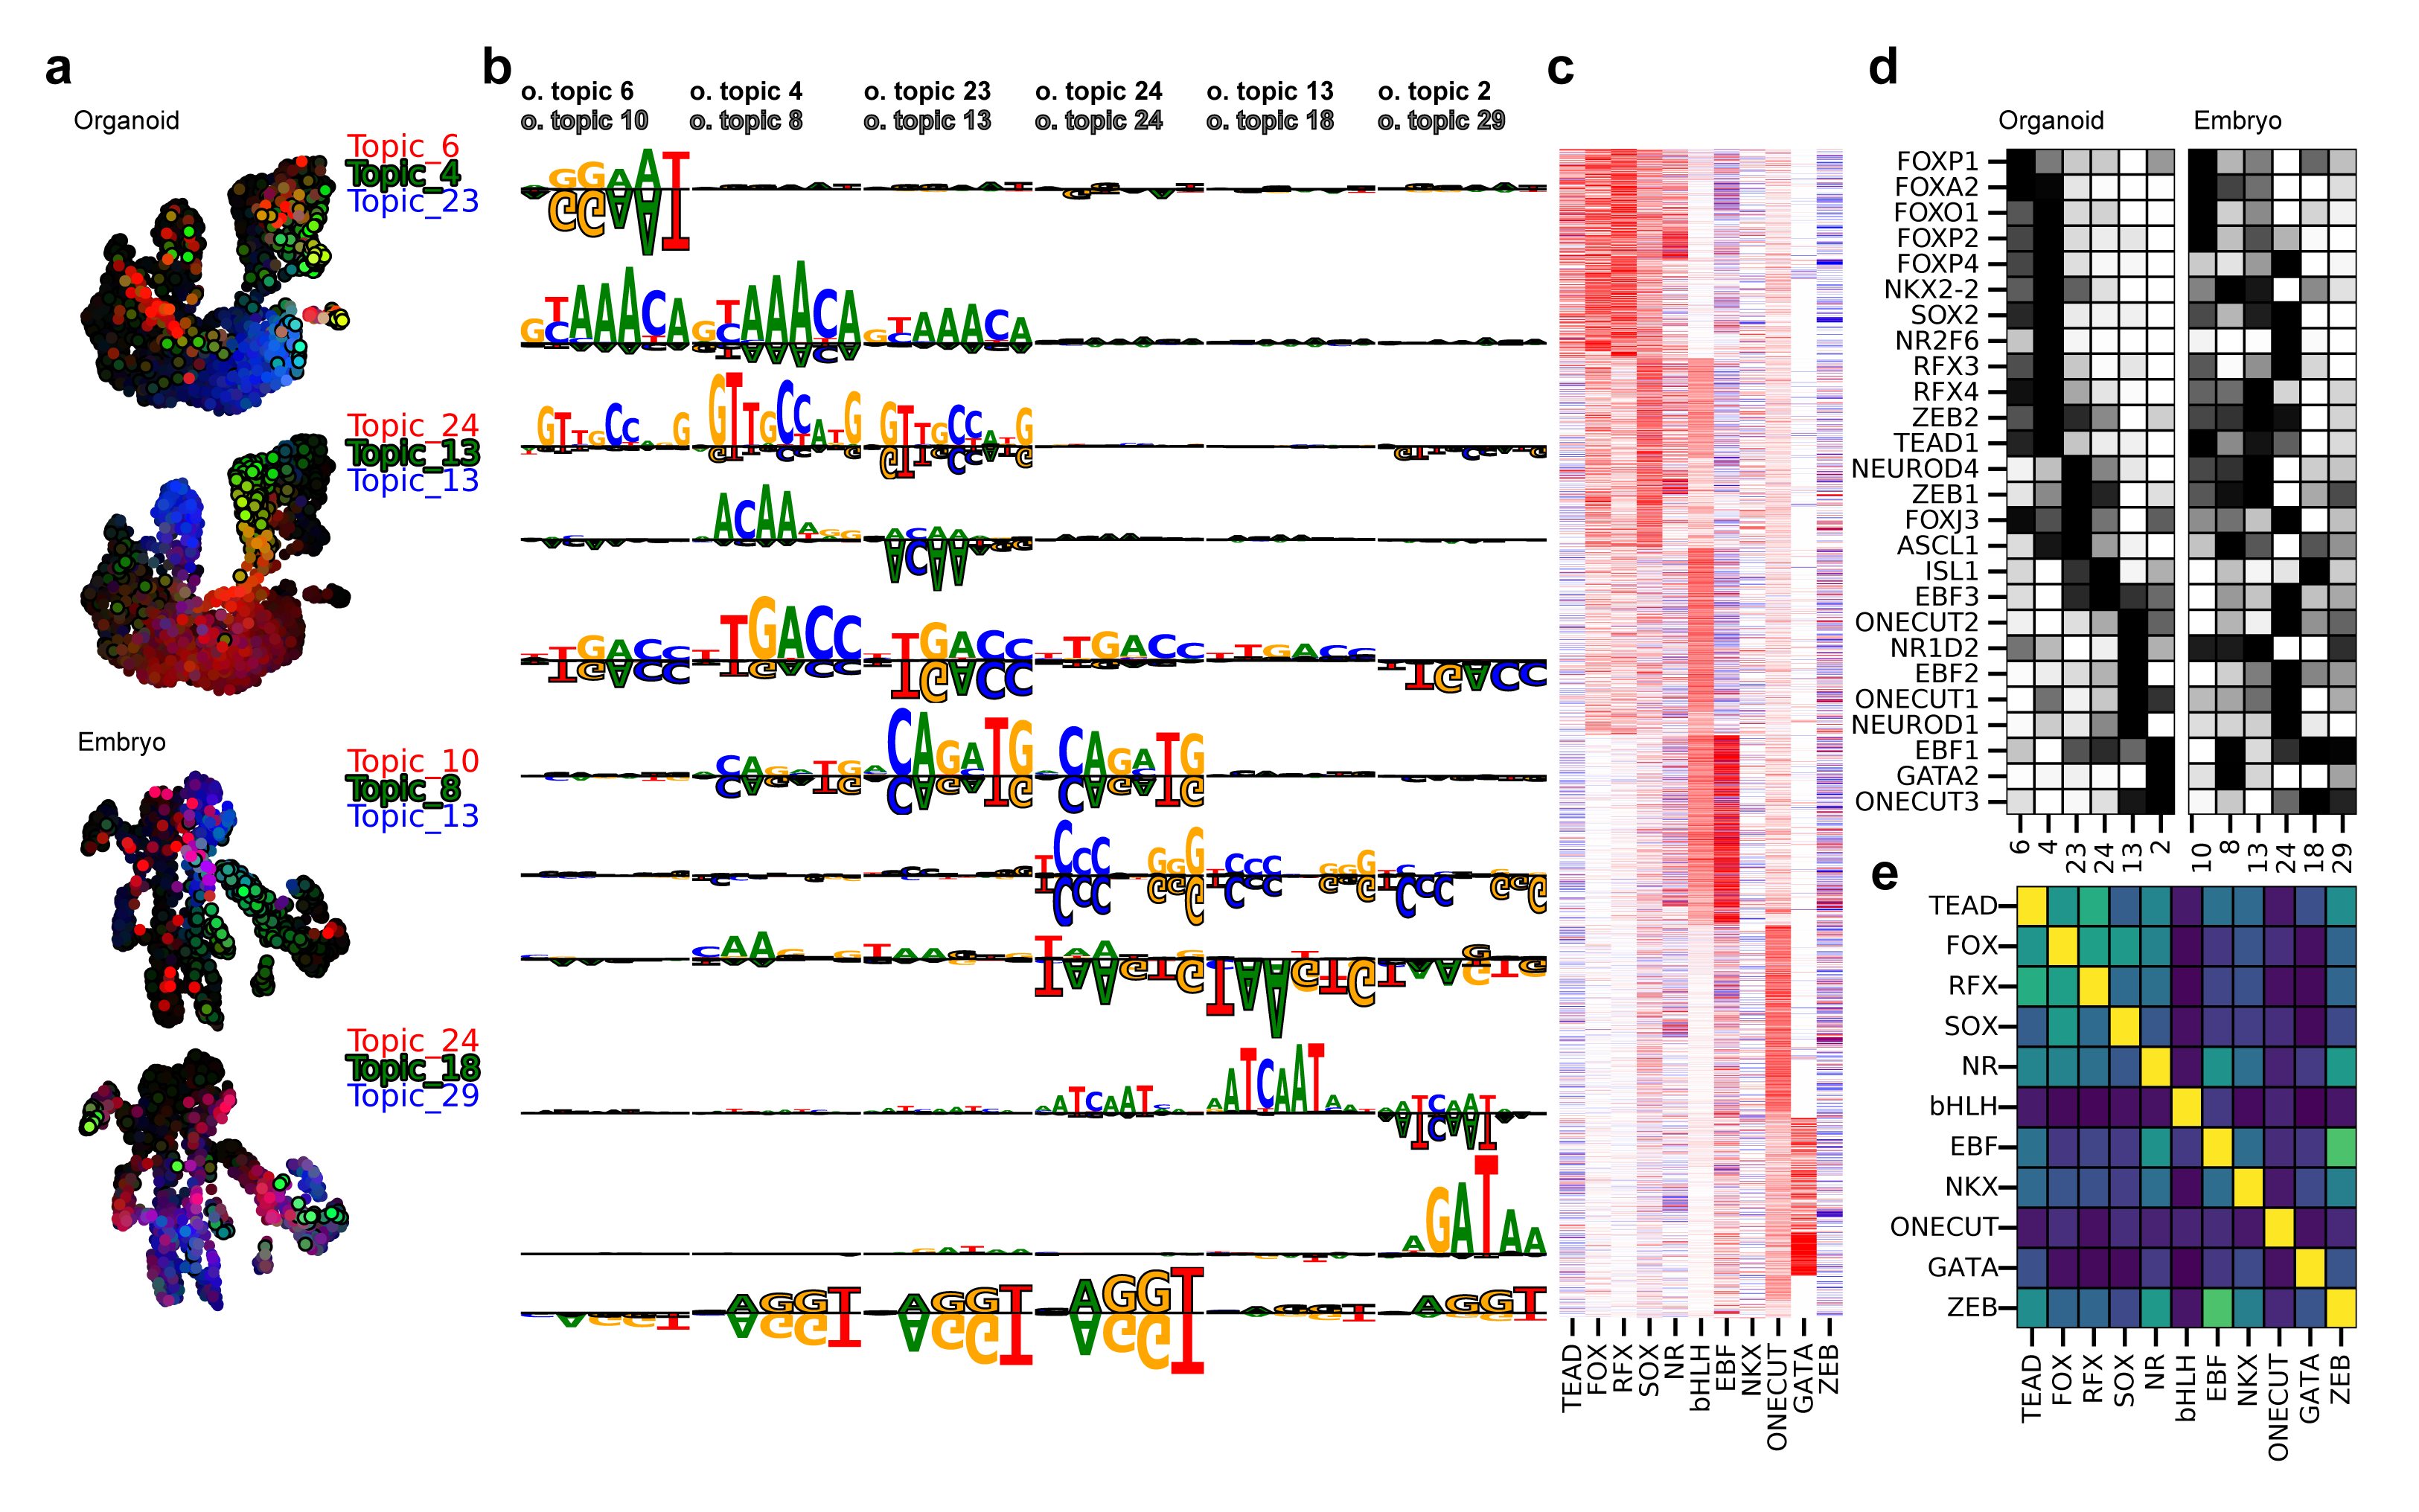
\includegraphics[width=1.0\linewidth]{figures/main/Figure_6.png}
  \captionsetup{justification=raggedright}
  \caption{ \textbf{Deciphering the enhancer code of early neuronal differentiation.} \\
 \textbf{a}, UMAP of organoid (top two) and embryo (bottom two) differentiating neuron cells colored by cell-topic probabilities in RGB color scales for neuron related topics. \textbf{b}, Code table showing average contribution score of pattern instances for each neuron related topic. Contribution scores for $DeepNeuralTube^o$ are not outlined. Contribution scores for $DeepNeuralTube^e$ are outlined and negated. \textbf{c}, Heatmap showing the maximum normalized contribution score for each of the top 1,000 regions per topic (y-axis) and pattern (x-axis) of neuron related topics. \textbf{d}, Heatmap showing scaled expression of transcription factors corresponding to identified patterns in organoid (left) and embryo (right) for neuon related topics. \textbf{e}, Heatmap showing Jaccard index of regions based on the presence of instances of the identified patterns.
  }
\end{figure}

\subsection* {
  Four to five distinct transcription factor binding sites in a region of around 140 base pairs is sufficient to encode
  all cell states related to neuronal progenitors, early neuronal differentiation and neural crest development.
}

Summarizing our results, we identified a total of sixteen and fifteen distinct cell states in 
respectively the neural tube organoids and the head of a four weeks post conception human embryo with 
almost one-to-one correspondence based on TFBS importances and TF expression. 
Additionally, we identified 4 distinct cell states corresponding to AP patterning of the neuronal progenitors 
in the embryo. To get insight into the minimal set of TFBS that are needed to encode these cell states we trained
logistic regression models to classify genomic regions as belonging to the topic representing each state or not,
making use of the motif scores of the identified patterns from each code table (\textbf{Fig. 3e}, \textbf{Fig. 4e}, \textbf{Fig. 5b} and \textbf{Fig. 6b}). 
The overall performance of these models was acceptably high (\textbf{Fig. 7a}) with an average auROC of 0.77 
and average auPR of 0.39. 
Notably, all models for neural crest related states performed best (\textbf{Fig. 7a}). 
Next, for each cell state, we selected TFBS that had a positive coefficient for at least one of the logistic regression models 
resulting in a total of twenty one TFBS for fifteen to sixteen states plus the additional four AP states (\textbf{Fig. 7a}). 
Finally, we used the identified TFBS to design synthetic enhancers for each state using motif embedding\cite{taskiranCelltypedirectedDesignSynthetic2024, kempynckCREstedModelingGenomic2025}. 
We used at least three TFBS in the design process for each state. 
In case less than three distinct TFBS had a positive coefficient for a state, we implanted multiple copies of each TFBS to come to a total of at least four TFBS. 
The resulting synthetic DNA sequences had an overall high prediction score (X.X on average) (\textbf{Fig. 7a}) - 
%TODO: add average prediction score
and were cell type specific (\textbf{Fig. 7b}) - with the prediction score for neural crest related states being again the highest. 
Note that some TFBS like FOX and SOX are used by many cell states (\textbf{Fig. 7a}) while other are more specific to certain states. \par

To conclude, our results indicate that enhancers specific to DV-patterning, neural crest states and early neuronal differentiation are encoded in the human genome using around four to five distinct TFBS (\textbf{Fig. 7a}) 
in regions of on average 134 - 154 bp in size (\textbf{Fig. 7c}), 
corresponding to the size of one nucleosome depleted region (NDR). 
AP-patterning enhancers seem to be an exception to this rule, where they are encoded using only two and sometimes even a single TFBS (\textbf{Fig. 7a}).

%TODO: number panels, in A middle, move legend so that text/lines do not class with guiding lines. Color for progenitor and neural crest are very similar and difficult to distinguish. I sometimes use this website to pick colors that are also colorblind friendly. https://colorbrewer2.org/#type=qualitative&scheme=Accent&n=4

\afterpage{\clearpage}
\begin{figure}[p]
  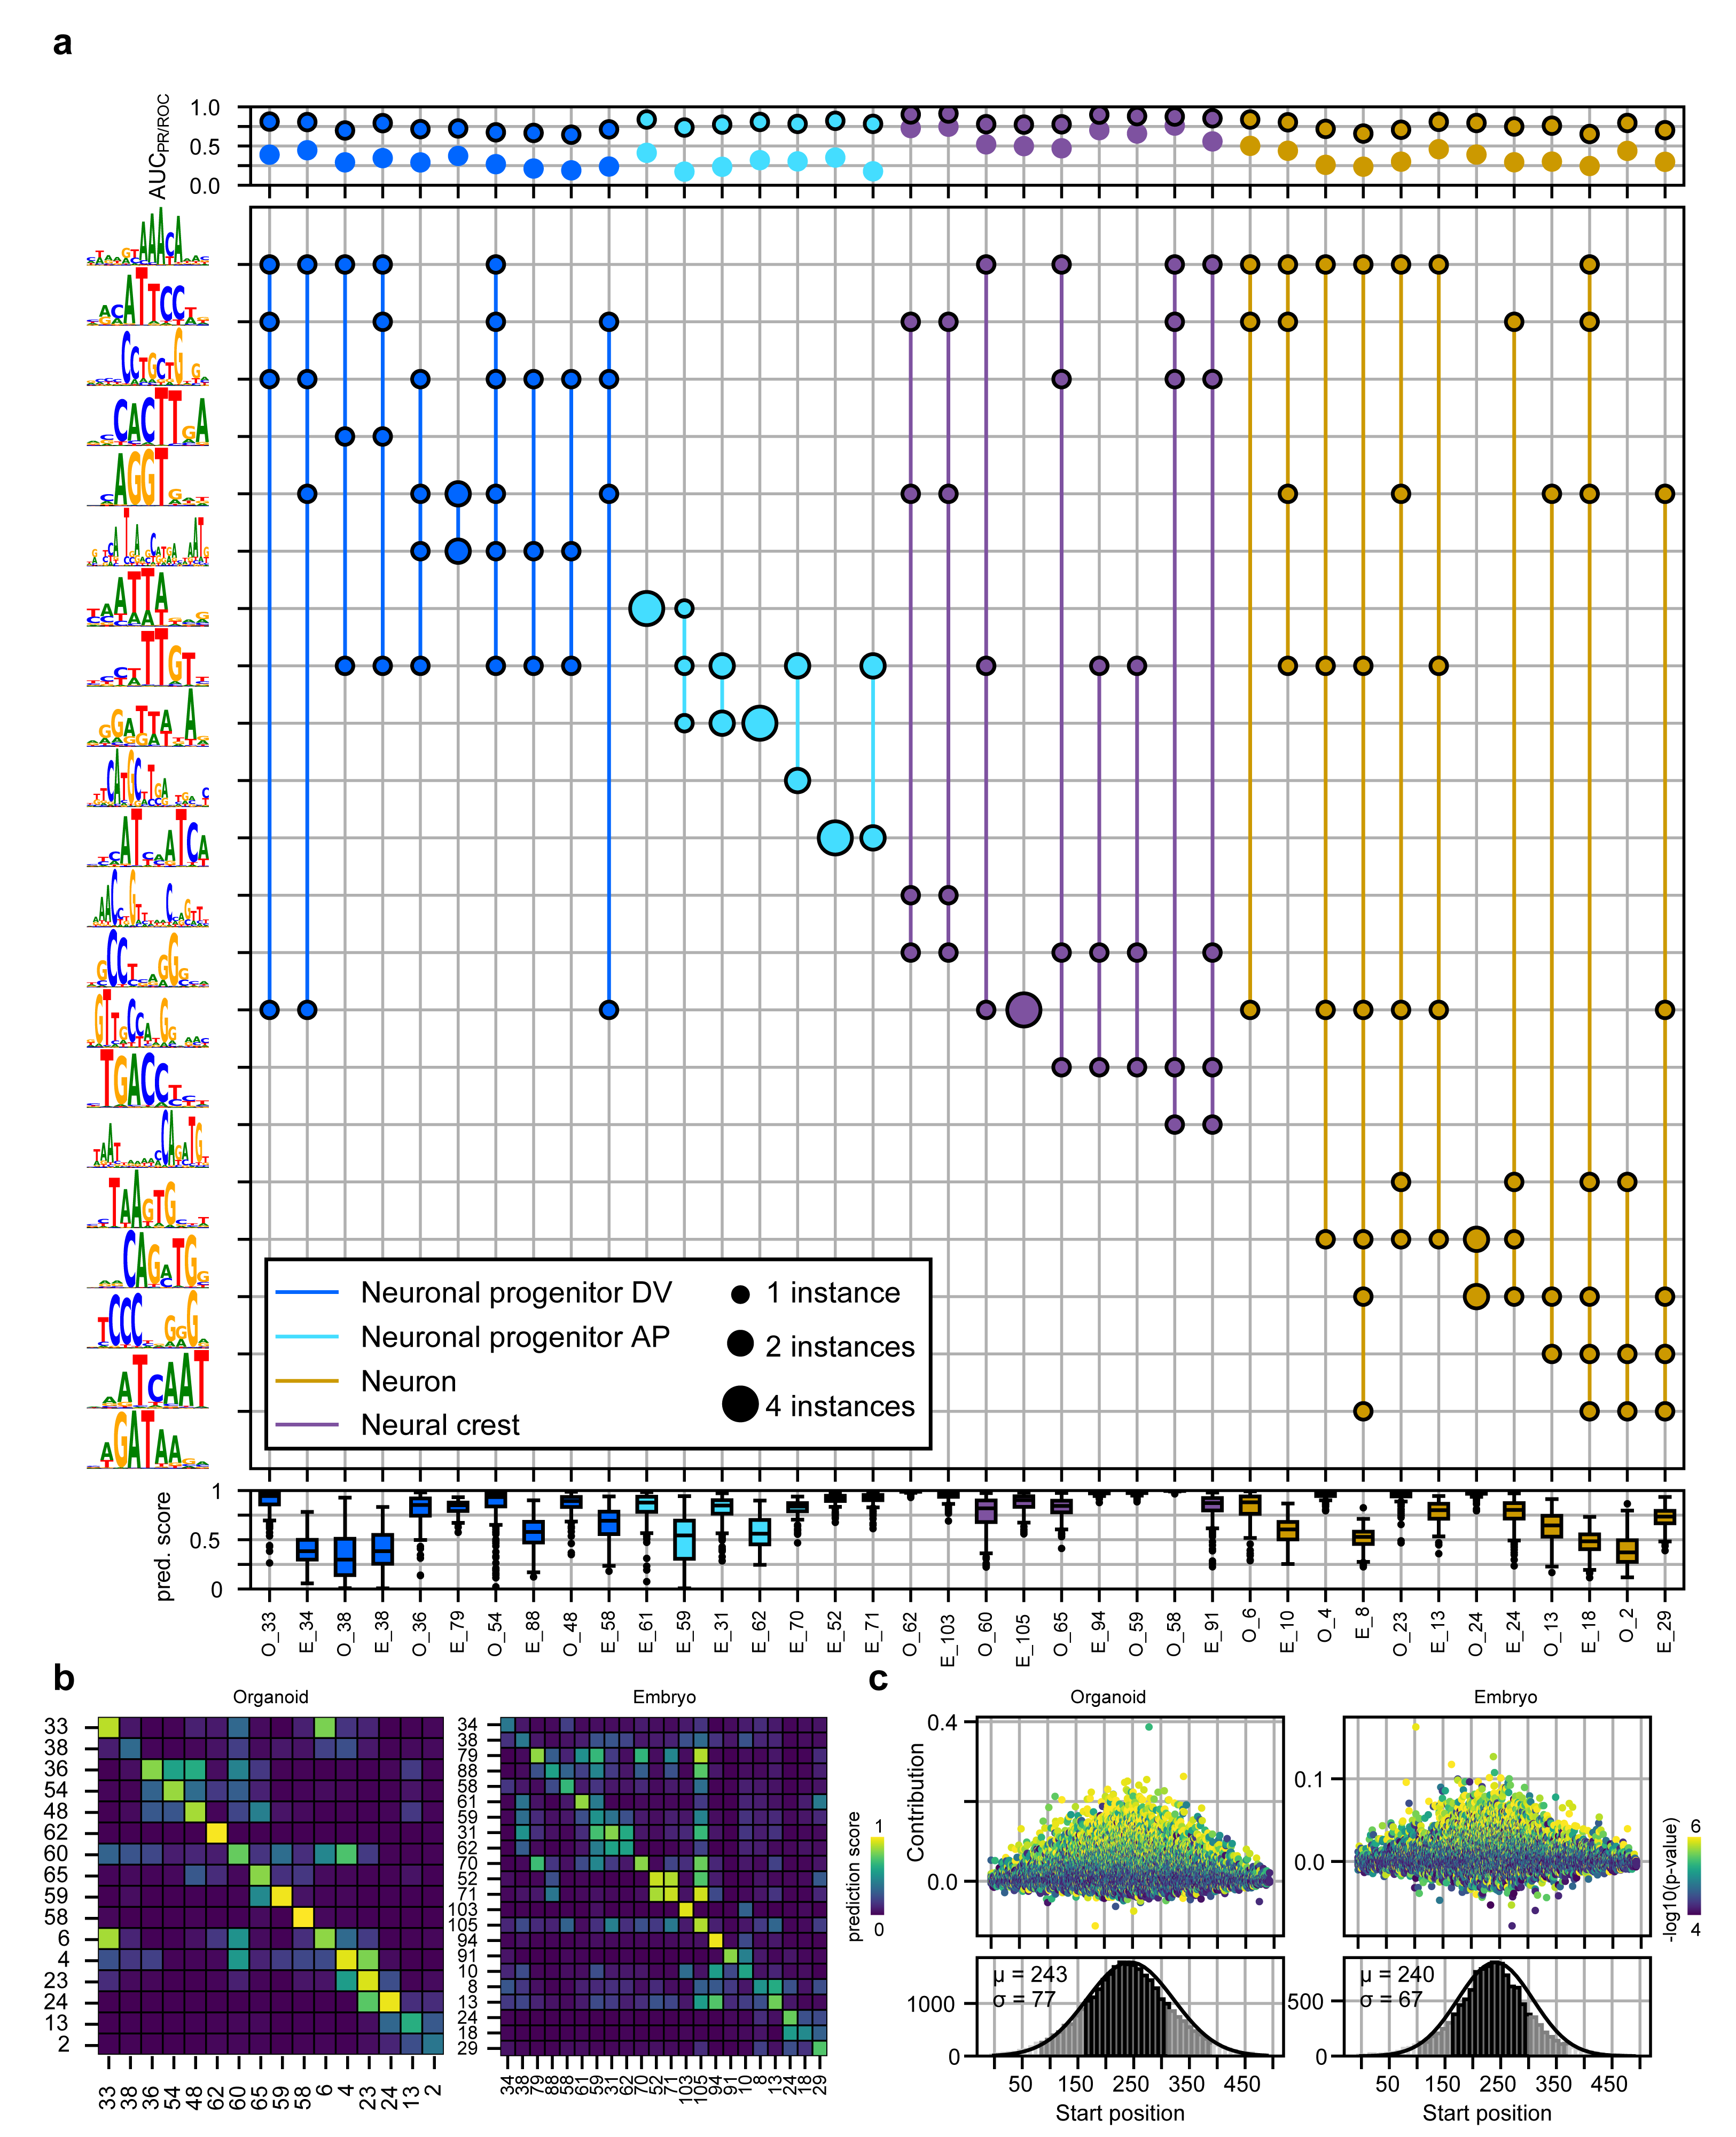
\includegraphics[width=1.0\linewidth]{figures/main/Figure_7.png}
  \caption{
    \textbf{Neural tube cell states are encoded using four to five distinct transcription factor binding sites} \\
\textbf{a}, Area under the receiver-operator curve (outlined dots) and precision-recall curve of logistic regression
models classifying genomic regions to each topic using motif scores as features (top) and patterns with positive
coefficient for each logistic regression model along with the number of each patterns used for enhancer design
represented by the size of each dot (middle) and boxplots (n = 200) showing prediction score of designed enhancers for
each topic (bottom). (Continues next page)}
\end{figure}
\afterpage{\clearpage}

\newpage
\vspace*{-\topskip}  
\begin{figure}[t]
  \ContinuedFloat
  %\caption*{\rule{\linewidth}{0.4pt}}
  \caption{
  (Continued)  \textbf{b}, heatmap showing prediction score for each topic of enhancers designed for all topics
for using $DeepNeuralTube^o$ (left) and $DeepNeuralTube^e$ (right). \textbf{c}, scatter plot showing
location of all pattern instances and contribution score at those locations, color is -log p value of the motif score
for each pattern calculated using FIMO\cite{grantFIMOScanningOccurrences2011, schreiberTangermemeBiologicalSequence2025} for organoid (top left) and embryo
(top right) and histograms showing the number of motif instances per 25 bp bins with confidence intervals indicated in
gray scales (black is +/- 1 standard deviation, gray is +/- 2 standard deviation and white is more than 3 standard
deviations) for organoid (bottom left) and embryo (bottom right).
}
\end{figure}



\clearpage
\section*{DISCUSSION}

%%% The discussion should explain the significance of the results and place them into a broader context.
%%% Subheadings are permitted.

We built a compendium of enhancer-codes underlying early human neuronal and neural crest development. 
Providing enhancer-codes of neuronal progenitor DV- and AP-patterning, 
early neuronal fate acquisition and 
neural crest induction, migration and facial mesenchyme specification.\par

To create this compendium, we generated a single-cell multiome (combined scATAC-seq and scRNA-seq of the same cell) 
dataset of the head of a four weeks post conception human embryo and we showed that the embryonic cell states can 
effectively be reproduced using human neural tube organoids on both transcriptomic level and on the level of the 
enhancer-codes. Specifically, we identified a total of fifteen distinct cell states with one-to-one matches between 
the organoid and embryo. The fact that cell states were defined in a data driven manner by making use of topic 
modeling and that each of these states were independently identified in two separate datasets increases the confidence 
of their biological relevance. Furthermore, this high similarity between the organoid and the embyro derived cell 
states validates neural tube organoids as a biological model for early human neural tube and neural crest development, 
biological cell states that are otherwise not easily accessible in humans.\par

The enhancer code remains complicated to study\cite{wassermanAppliedBioinformaticsIdentification2004} especially
compared to the genetic code\cite{kimDecipheringMultiscaleQuantitative2023, deboerHoldOutGenome2024}. 
Nonetheless, there are recurrent patterns that are shared among enhancers of different cell types. 
In particular, enhancers underlying DV patterning, early neuronal fate acquisition and neural crest 
tend to consist of heterotypic clusters of 4-5 different TFBS\cite{kimDecipheringMultiscaleQuantitative2023, longEverChangingLandscapesTranscriptional2016} that are located within one NDR (+/-147bp). 
That is to say, cooperative binding of multiple TFs underlies the cell type specificity of enhancers\cite{lambertHumanTranscriptionFactors2018}. 
Here, we see most evidence for a model of indirect cooperativity\cite{longEverChangingLandscapesTranscriptional2016} (i.e., flexible billboard enhancer model\cite{arnostiTranscriptionalEnhancersIntelligent2005}). 
However, for multiple cell types we also observed evidence of direct coooperativity between TFs in the form of protein-protein interactions between two TFs. 
This was the case for TWIST1 and homeodomain TFs heterodimers in facial mesenchyme\cite{kimDNAguidedTranscriptionFactor2024} 
and GRHL1/2 dimers, 
TFAP2A and TFAP2B/C heterodimers\cite{rothsteinHeterodimerizationTFAP2Pioneer2020} 
and SOX10 homodimers in neural crest. 
For all these TFs we found dimer motifs with a fixed number of nucleotides in between the two TFBS instances. 
Of note, for SOX10 we observed three different dimer motif with either 3, 4 or 5 bps spacing,
with instances with 4 bps spacing being the most accessible (\textbf{Supplementary Fig. 8}). 
Finally, we also observed evidence of pioneer activity, where binding of one TF can facilitate the 
subsequent binding of other TFs to the same enhancer\cite{longEverChangingLandscapesTranscriptional2016}. 
This was the case for FOXA2 in the floorplate, consistent with previous findings of FOXA TFs\cite{iwafuchi-doiPioneerTranscriptionFactor2016, iwafuchiGeneNetworkTransitions2020}. 
Others have hypothesized, however, that pioneer activity is not a qualitative feature of a TF but rather 
dependent on the affinity of interactions between TF and DNA\cite{hansenTestPioneerFactor2022}. 
Similarly, we observed that enhancers that are specific to the floorplate contain either less FOXA2 binding sites 
and/or binding sites of lower affinity. 
The use of suboptimal TFBS is a reoccurring feature of cell type specific enhancers\cite{farleySuboptimizationDevelopmentalEnhancers2015, crockerChapterTwentySevenSoft2016, limAffinityoptimizingEnhancerVariants2024, naqviTransferLearningReveals2025}.\par
%TODO: S.A.: But retain strongest footprint ?!
Our results indicate that enhancers underlying neuronal progenitor AP-patterning form an exception to the rule 
that enhancers consist of clusters of 4-5 different TFBS. 
Homotypic clusters of 3-4 homeobox instances were sufficient to both create and identify enhancers specific to a certain AP domain. 
Similar findings were already reported in fly\cite{crockerLowAffinityBinding2015}. 
It has been a long standing question how homeodomain TFs achieve specific binding\cite{mannChapter3Hox2009, hubertHoxGenesDevelopment2023} 
given that all homeodomain TFs seem to bind the same \textit{TAAT} motif\cite{bergerVariationHomeodomainDNA2008, noyesAnalysisHomeodomainSpecificities2008}. 
It has been hypothesized that specificity is mainly achieved through cooperative binding with other TFs\cite{mannChapter3Hox2009}. 
Indeed, we observe this for EN1/2 and HOXB3 that are predicted to co-bind with PAX5/8 and MEIS1/2 or PBX1/3 respectively forming specific dimer motifs.
In contrast, we suggest a novel mode where specificity is achieved through the homeodomain itself for respectively LHX2/9, RAX or SIX3/6 and OTX1/2, EMX2, DMBX1 or LMX1A 
that preferentially bind \textit{TAATTA} and \textit{TAATCC} sites. 
Thus, additional nucleotides, next to the core \textit{TAAT}, form a TFBS that is both necessary and sufficient for genome wide cell type specificity. 
In general, although there are only around 100 different DNA binding domains across human TFs\cite{lambertHumanTranscriptionFactors2018} 
and thus many of the 1,639 known human TFs recognize similar motifs\cite{lambertHumanTranscriptionFactors2018} 
there are slight variations in preferential TFBS of TFs of the same family\cite{lambertHumanTranscriptionFactors2018, jolmaDNABindingSpecificitiesHuman2013, dealmeidaDeepSTARRPredictsEnhancer2022} 
that could be important for cell type specific binding.\par

In conclusion, we provide an enhancer-code compendium of early human neuronal and neural crest development. 
We confirm the paradigm that enhancers consist out of heterotypic clusters of TFBS with soft syntactic rules 
but also provide a counter example to this paradigm. 
Furthermore, we validate the biological relevance of neural tube organoids. 
Finally, we provide $DeepNeuralTubes$, two sequence-to-chromatin accessibility models, 
freely available to the research community, 
which can be used to predict, 
interpret and design enhancers underlying early human neuronal and neural crest development.

% single TF
% https://genome.cshlp.org/content/26/7/882.short

%% position of the binding sites vis a vi nucleosomes
% https://www.pnas.org/doi/abs/10.1073/pnas.1804663115

%% Repression through chromatin closing
% carmen paper & ibrahim paper

%% what about repression through chromatin opening

% another paper of face GWAS: https://www.nature.com/articles/s41588-018-0057-4

% white box models
% DeepNeuralTube
% AP patterning (TP53)
% interpretation of human variation

\subsection*{Limitations of the study}

%%% A "limitations" or "limitations of the study" subsection in the discussion is encouraged and may be required for some
%%% journals and some article formats.

In this study we focused on predicting TF binding to enhancers, but not so much on their effector function. 
The effect a TF has on target gene expression depends on its effector domain and interactions with
co-factors\cite{lambertHumanTranscriptionFactors2018} and this may depend on the sequence context of
the enhancer itself\cite{jacobsWidespreadRegulatorySpecificities2023}. 
Large scales studies, in a variety of cell states, are now being performed to map TFs to co-factors and downstream effects on gene expression\cite{
  tyckoHighThroughputDiscoveryCharacterization2020, alerasoolIdentificationFunctionalCharacterization2022,
sotoCompendiumHumanTranscription2022, delrossoLargescaleMappingMutagenesis2023,
mukundHighthroughputFunctionalCharacterization2023, bellComparativeCofactorScreens2024,
tyckoDevelopmentCompactTranscriptional2024, doughtySinglemoleculeStatesLink2024}. 
These studies may especially be important to infer repressive roles of TFs on gene expression, 
an effect that is currently difficult to study with state of the art methods\cite{bravogonzalez-blasSCENICSinglecellMultiomic2023, kempynckCREstedModelingGenomic2025,
dewinterModellingDesignTranscriptional2025}. 
In particular for the neural tube, it is known that repressive interactions in its core GRN are important\cite{delasRepressiveInteractionsGene2020}. 
In this study we could only predict a strong repressive effect of ZEB2, a chromatin closing repressor that is used across a variety of biological
systems\cite{minnoyeCrossspeciesAnalysisEnhancer2020, taskiranCelltypedirectedDesignSynthetic2024}
(\textbf{Supplementary Fig. S9}).\par

Furthermore, the expression of a gene is in general regulated by multiple enhancers in the gene's locus\cite{
  perryShadowEnhancersFoster2010,
martinez-araSystematicAnalysisIntrinsic2022, bergmanCompatibilityRulesHuman2022, zuinNonlinearControlTranscription2022,
gschwindEncyclopediaEnhancergeneRegulatory2023, martinez-araLargescaleAnalysisIntegration2024,
loubiereDevelopmentalHousekeepingTranscriptional2024, thomasEnhancerCooperativityCan2025}.
In this study we focused on the enhancer code of individual enhancers 
but not how the signal of multiple enhancers is integrated to control target gene expression. 
Currently efforts are ongoing to build large scale models for modeling gene expression making use of the
code of all enhancers in the gene's locus\cite{avsecEffectiveGeneExpression2021,linderPredictingRNAseqCoverage2025a,
hingerlScoobyModelingMultimodal2024, hingerlFlashzoiEnhancedBorzoi2024, lalDecodingSequenceDeterminants2025}.\par

To conclude, we suspect that future models will need to take into account both the effector function of TFs through
modeling co-factor interactions and the entire gene's locus (including all enhancers and promoter(s)) to effectively
model GRNs underlying the cell's transcriptome.

\newpage


%%%  The following components should appear after the 
%%%  methods. 
%%%  For journals using STAR Methods, these components 
%%%  should appear immediately after the discussion 
%%%  (after any "limitations" or "conclusions" subsection 
%%%  within the discussion).

\section*{RESOURCE AVAILABILITY}

%%%  The resource availability section is required 
%%%  for all research articles. This component 
%%%  has 3 subsections: "lead contact," "materials 
%%%  availability," and "data and code availability." 
%%%  All 3 subsections must be included, even if no 
%%%  unique materials were generated in the study. 
%%%  Do not edit or change the names of the subheadings. 
%%%  No other subheadings or text are allowed in the 
%%%  resource availability section.

\subsection*{Lead contact}

%%%  Authors are required to designate a lead contact, 
%%%  who will be responsible for communication with 
%%%  the journal before and after publication and is 
%%%  the arbiter of disputes, including concerns 
%%%  related to reagents or resource sharing. Only 
%%%  one author can be named the lead contact, and 
%%%  only the lead contact’s information may be 
%%%  provided in this section.

Requests for further information and resources should be directed to and will be fulfilled by the lead contact, Stein Aerts (stein.aerts@kuleuven.be).

\subsection*{Materials availability}

%%%  This subsection must include a statement describing 
%%%  the availability of newly generated materials 
%%%  associated with the paper, including any conditions 
%%%  for access. If there are no newly generated materials 
%%%  associated with the paper, the statement should 
%%%  state this, e.g.: This study did not generate new 
%%%  materials.

This study did not generate new materials

\subsection*{Data and code availability}

%%%  All original research papers must include a 
%%%  comprehensive and accurate “data and code 
%%%  availability” statement within the “resource 
%%%  availability” component of the paper before it 
%%%  is accepted for publication. These statements 
%%%  are structured and consist of three bulleted 
%%%  components. Each component must be present.

\section*{ACKNOWLEDGMENTS}

%%%  Use this section to acknowledge contributions 
%%%  from non-authors and list funding sources, 
%%%  including grant numbers.
\section*{AUTHOR CONTRIBUTIONS}

%%%  This component is required for most research papers. 
%%%  Mention each individual author with a statement 
%%%  outlining the contribution of each author to the work.

\begin{itemize}
  \item Conceptualization: S.D.W. \& S.A.
  \item Experiments and sample preparation: S.D.W., V.C., E.S., L.H. \& C.M.
  \item Computational analysis: S.D.W. \& C.M.
  \item Writing – original draft: S.D.W. \& S.A.
  \item Writing – review \& editing:
\end{itemize}

\section*{DECLARATION OF INTERESTS}

%%%  This component is required for all articles, even 
%%%  if the authors have no competing interests; if 
%%%  this is the case, insert "The authors declare no 
%%%  competing interests." Please refer to the 
%%%  declaration of interests policy: 
%%%  https://www.cell.com/declaration-of-interests

\section*{DECLARATION OF GENERATIVE AI AND AI-ASSISTED TECHNOLOGIES}

%%%  If generative AI and AI-assisted technologies 
%%%  were used in the writing process, this must 
%%%  be disclosed in the paper. This declaration 
%%%  does not apply to the use of basic tools for 
%%%  checking grammar, spelling, references, etc. 
%%%  If you have nothing to disclose, please do not 
%%%  include this component.

During the preparation of this work, the author(s) did not make use of generative AI.

\section*{SUPPLEMENTAL INFORMATION INDEX}

%%%  Supplemental information must be uploaded as 
%%%  separate files. In the main text, please list the 
%%%  files to be included in a brief index. For details, 
%%%  please review the supplemental information guidelines: 

%%%  Journals with a general "methods" section: 
%%%  http://www.cell.com/supplemental-information

%%%  Journals with STAR Methods: 
%%%  https://www.cell.com/STAR-supplemental-information

%\begin{description}
%  \item Figures S1-S5 and their legends in a PDF
%  \item Table S1. A descriptive title for an Excel file that was too large to appear in the PDF
%  \item Table S2. Another descriptive title for a different Excel file
%  \item Data S1. Raw data on x, y, and z
%\end{description}

\newpage

\section*{MAIN FIGURE TITLES AND LEGENDS}

%%%  At final submission, figure files MUST be 
%%%  provided separately as high-resolution image 
%%%  files. All of the panels for a figure should 
%%%  be in the same file. Figures should have 
%%%  clear labels/file names (Figure 1, Figure 2, 
%%%  etc.). 

%%%  Figure titles and legends should be placed 
%%%  at the end of the main text. You do not 
%%%  need to place the figures, nor their titles 
%%%  and legends, within the main text. While 
%%%  typesetting your article, our team will 
%%%  place each figure in the best location 
%%%  based on the final layout and on your 
%%%  figure citations, e.g., (Figures 1A and 1B). 

%%%  Please review the figure guidelines before 
%%%  submitting your final materials: 
%%%  https://www.cell.com/figureguidelines.

\newpage

\section*{MAIN TABLES, INCLUDING TITLES AND LEGENDS}

%%%  Whenever possible, we encourage you to submit 
%%%  your main-text tables as Microsoft Word documents, 
%%%  using Word's table function. This will ensure 
%%%  the best results during conversion. Tables 
%%%  should be numbered Table 1, Table 2, etc. and 
%%%  should not include subpanels (do not use Table 1A, 
%%%  1B, etc.). Give each table a brief descriptive 
%%%  title. Table legends are optional but encouraged. 
%%%  Footnotes (superscript lowercase letters) should 
%%%  be used where necessary to indicate some feature 
%%%  of the data; please do not use bold, italic, 
%%%  colored text, or shading for this purpose. Use 
%%%  separate cells, not line breaks or spaces, for 
%%%  all discrete data elements. Small embedded 
%%%  graphics with color are OK.

%%%  Like figures, all tables must be cited within 
%%%  the main text, and our typesetting team will 
%%%  place the tables within the typeset paper at 
%%%  the appropriate locations.


%\subsection*{Table 1. A table with clear organization of data}

%\begin{tabular}{|l | l | l | l|} 
% \hline
% \textbf{Column 1} & \textbf{Column 2} & \textbf{Column 3} & \textbf{Column 4} \\ [1ex] 
% \hline
% Row A\textsuperscript{a} & 6 & 87,837 & 787 \\ [1ex] 
% \hline
% Row B & 7 & 78 & 5,415 \\ [1ex] 
% \hline
% Row C & 545 & 778 & 7507 \\ [1ex] 
% \hline
% Row D & 545 & 18,744 & 7,560 \\ [1ex] 
% \hline
% Row E & 88 & 788 & 6,344 \\ [1ex] 
% \hline
%\end{tabular}

\bigskip

%The table legend (optional) follows the table itself. The legend should be used to provide additional info that relates to the table as a whole.

%textsuperscript{a}Footnotes can be used to provide additional info on specific content within the table, such as this footnote to the first row (row A). Do not use footnotes in the table title.

%\textsuperscript{b}More footnotes

\newpage

%%%  REFERENCES: As of 2023, all Cell Press journals 
%%%  use Numbered (AMA) style. We recommend placing 
%%%  your references in the included "references.bib" 
%%%  file.


\bibliography{references}



\bigskip

%%%  In your References, please include only articles 
%%%  that are published (online publication and 
%%%  preprint servers are OK). Unpublished data, 
%%%  submitted and/or accepted manuscripts, abstracts, 
%%%  and personal communications should be cited within 
%%%  the text only ("unpublished data," "data not 
%%%  shown," "Alice Smith, personal communication") 
%%%  and not included in the references list. Personal 
%%%  communication should be documented by a letter 
%%%  of permission. Whenever possible, please make 
%%%  sure your .bib file has the complete author lists 
%%%  for each item (at minimum, the first 11 authors 
%%%  listed). 

\newpage


%All Cell Press \textbf{life and medical science} journals, and the multidisciplinary journal \textbf{iScience}, use the \textbf{\href{https://www.cell.com/star-authors-guide}{STAR Methods}} format for reporting materials and methods. Other Cell Press journals use a non-structured \textbf{methods} format; for those journals, please \textbf{delete} the contents of this page from the template and refer instead to the \textbf{methods} template on page 3.

%f you are publishing in a STAR Methods journal, please refer to the appropriate guide for authors:
%\begin{itemize}
%\item \textit{Cell} authors should download the guide for \textit{Cell} authors \href{https://www.cell.com/pb-assets/journals/research/cell/methods/Methods_Guide_Cell-1678470557763.pdf}{available here}
%\item All other journal authors should use \href{https://www.cell.com/pb-assets/journals/research/cell/methods/Methods_Guide_general-1678470557763.pdf}{this version of the guide}
%\end{itemize}


\section*{STAR METHODS}

%%%  The STAR Methods should appear in your main 
%%%  manuscript file after the figure legends, main 
%%%  table(s) and table legend(s).

\subsection*{Key resources table}

%\textit{To create the KRT, please use the \href{https://star-methods.com}{KRT webform} or the \href{http://www.cell.com/pb-assets/journals/research/cell/methods/table-template1.docx}{Word template} and upload this file separately.}



\subsection*{Experimental model and study participant details}

%%%  Please list here under separate headings 
%%%  all the experimental models/study participants 
%%%  (animals, human participants, plants, microbe 
%%%  strains, cell lines, primary cell cultures) 
%%%  used in the study. For each model, provide 
%%%  information related to their species/strain, 
%%%  genotype, age/developmental stage, sex (and 
%%%  gender, ancestry, race, and ethnicity if 
%%%  reported for human studies), maintenance, 
%%%  and care, including institutional permission 
%%%  and oversight information for the studies 
%%%  the experimental animal/human participant 
%%%  study. The influence (or association) of sex, 
%%%  gender, or both on the results of the study 
%%%  must be reported. In cases where it cannot, 
%%%  authors should discuss this as a limitation 
%%%  to their research’s generalizability.

%%%  Please omit this component if your study does 
%%%  not use experimental models typical in the 
%%%  life sciences (e.g., if your study is 
%%%  computational or physical science research). 

\subsubsection*{Collection of human fetal samples}

The experiments on human embryos in this study fall under category 2 as defined by the International Society for Stem
Cell Research (ISSCR) 2021 guidelines. All experiments followed relevant guidelines and regulations, including the ISSCR
2021 guidelines. Human fetal samples were collected from routine termination of pregnancies at the Karolinska University Hospital following informed consent of the donors. The donors were informed of the purpose of the research and specific procedures the tissues will be used for. The use of fetal samples collected from abortions was approved by the Swedish Ethical Review Authority and the National Board of Health and Welfare (Etikprövningsmyndigheten; DNR2020-02074). Embryos were not kept in culture and were immediately dissected after collection. The embryo was staged according to the Carnegie stages. Following the dissection, the samples were transferred to ice-cold Hibernate E medium (ThermoFisher, A1247601) and processed the same day.

\subsubsection*{Generation of human neural tube organoids}
The generation of human neural tube organoids falls under category 1a as defined by the ISSCR 2021 guidelines. 
Two induced Pluripotent Stem Cell lines (iPSC): IPSC EPITHELIAL-1 (\href{https://rrid.site/data/record/SCR_013869-1/CVCL_EE38/resolver?q=SIGi001-A&l=SIGi001-A&i=rrid:cvcl_ee38-ebisc-sigi001-a}{RRID:CVCL\_EE38}; Purchased from Sigma-Aldrich iPSC0028 and hereafter referred to as Sigma iPSC), BJ1 iPSC (iPSC generated from BJ fibroblasts (\href{https://rrid.site/data/record/SCR_013869-1/CVCL_3653/resolver?q=CRL-2522&l=CRL-2522&i=rrid:cvcl_3653-atcc-crl-2522}{RRID:CVCL\_3653}) and kindly gifted by professor Catherine Verfaillie (Leuven Stem Cell Institute)) and one human Embryonic Stem Cell (ESC) line H9-ESC (\href{https://rrid.site/data/record/SCR_013869-1/CVCL_9773/resolver?q=NIHhESC-10-0062&l=NIHhESC-10-0062&i=rrid:cvcl_9773-0}{RRID:CVCL\_9773} and kindly gifted by professor Pierre Vanderhaeghen) were used for the \textit{in vitro} generation of human neural tube organoids.
The identities of the cell lines were validated based on their genomic sequences (see Methods details below).
Pluripotent stem cells were cultured in flat bottom, TC-treated 6 well plates (Avantor; 734-2323). For culture details see
Methods details below. 
All human iPSC and ESC experiments were approved by the Ethical Committee of the KU Leuven (ECD S63316)
. Human neural tube organoids were generated based on Fattah \textit{et al.} 2021 Nature communications\cite{
abdelfattahActuationEnhancesPatterning2021} and Ranga \textit{et al.} 2016 PNAS\cite{rangaNeuralTubeMorphogenesis2016}.
At 60-70\% confluency pluripotent stem cells were washed twice using Phosphate Buffered Saline
(PBS; ThermoFisher, 14190169; 2ml) next a single cell suspension was made by adding 1ml of room temperature TrypLE
Express Enzyme (ThermoFisher, 12605010) and incubation for 3 minutes at \SI{37}{\degreeCelsius} followed by pipetting up and down using a
\SI{1}{\milli\litre} pipette. Immediately after the TrypLE reaction was inhibited by adding \SI{2}{\milli\liter} of DMEM/F12 FBS (Fetal Bovine Serum (FBS; ThermoFisher, A5256701) \SI{20}{\percent} V/V; Penicillin-Streptomycin (ThermoFisher, 15140122) \SI{50}{\micro\gram} in DMEM/F12 (ThermoFisher, 11320033)). Cells were pelleted at 300 RCF for \SI{3}{\minute} and after counting on a LUNA-FL Dual Fluorescence Cell Counter resuspended to \SI{3.5e6}{cells\per\milli\litre} in $GM_0$ ( basal GM (N-2 Supplement (ThermoFisher, 17502048) 1x, B-27 Supplement (ThermoFisher, 17504044) 1x, GlutaMax Supplement (ThermoFisher, 35050061) 1x, Sodium Pyruvate (ThermoFisher, 11360070) \SI{1}{\milli\molar}, MEM Non-Essential Amino Acids Solution (ThermoFisher, 11140050) 1x, Penicillin-Streptomycin (ThermoFisher, 15140122) \SI{50}{\micro\gram\per\milli\litre}, Neurobasal Medium (ThermoFisher, 21103049) \SI{50}{\percent} V/V and DMEM/F12 (ThermoFisher, 11320033) \SI{50}{\percent} V/V) with RHO/ROCK inhibitor (Y-27632 (Dihydrochloride), Stemcell technologies, 100-1044) \SI{1}{\micro\molar}). Next, the polyethylene glycol A (PEG-A) hydrogel matrix (see Methods detail below) was prepared by first adding Corning Mouse Laminin (Avantor, 734-1098) \SI{0.1}{\milli\gram\per\milli\liter} followed by activated factor 13 (see Methods details below) in that order to a PEG mixture (see Methods details below; PEG \SI{1.5}{\percent} or \SI{2}{\percent} V/V, buffer (TRIS \SI{0.05}{\milli\molar}, $CaCl_2$ \SI{0.05}{\milli\molar}; pH 7.6; filter sterilized) in $GM_0$ medium). After mixing the matrix by pipetting up and down, without generating bubbles, for 1-2 minutes \SI{3.5e4}{cells\per\micro\litre} mixture were added. The matrix and gell mixture was mixed gently one more time by pipetting and \SI{10}{\micro\litre} droplets were generated in each well of a TC-treated 96 well plate (Corning, 3603). When the matrix started to gell the plate was turned up-side down for 10 seconds, after which it was turned right-side up for 10 seconds. This was repeated for a total of 5 times, after which the plates were kept at room temperature. After 20 minutes of gelling \SI{200}{\micro\litre} of $GM_0$ medium was added to each well and the organoids were incubated at \SI{37}{\degreeCelsius} \SI{5}{\percent} $CO_2$ for a total of 11 days, or until the timepoint of single-cell multiome. At day 3 of differentiation medium was changed with basal GM supplemented with retinoic acid (Sigma-Aldrich, R2625-100MG) \SI{0.25}{\micro\molar} and Smoothened agonist (Sigma-Aldrich, 566661-500UG) \SI{1}{\micro\molar}. At day 5, 7 and 9 the medium was changed with basal GM. 

\subsubsection*{Chicken embryos}
Fertilized chicken eggs, obtained from "Kwekerij van het Hallerbos" were incubated at \SI{37}{\degreeCelsius} at \SI{70}{\percent} humidity for 30 hours to reach Humburger Hamilton (HH) stage 4. Afterwards, embryos were removed from the egg and kept in culture for an additional 24 hours.

\subsection*{Method details}

%%%  Please provide precise details of all the 
%%%  procedures in the paper (behavioral task, 
%%%  generation of reagents, biological assays, 
%%%  modeling, etc.) such that it is clear how, 
%%%  when, where, and why procedures were 
%%%  performed. We encourage authors to provide 
%%%  information related to the experimental 
%%%  design as suggested by NIH and ARRIVE 
%%%  guidelines (e.g., information about 
%%%  replicates, randomization, blinding, sample 
%%%  size estimation, and the criteria for 
%%%  inclusion and exclusion of any data or 
%%%  subjects).

\subsubsection*{Human neural tube organoid culture}

\paragraph*{Factor 13 activation}
\SI{1}{\units} of reconstituted Thrombin (Sigma-Aldrich, 10602400001) in Ehrbars buffer (TRIS \SI{10}{\milli\molar}; NaCl
\SI{150}{\milli\molar}; $CaCl_2$ \SI{25}{\milli\molar}; pH 7.4) per \SI{90}{\units} of reconstituted Fibrogammin (UZ Leuven pharmacy)
was mixed and put in water bath at \SI{37}{\degreeCelsius} for 30 minutes while swirling every 5 minutes. Activated
factor 13 was filter sterilized, aliquoted and stored at \SI{-80}{\degreeCelsius}.

\paragraph*{PEG-A hydrogel precursor synthesis}
PEG-A hydrogel precursors, as described in Ranga \textit{et al.} nature
communications\cite{ranga3DNicheMicroarrays2014}, were kindly gifted by professor Adrian Ranga (Department of Mechanical
Engineering at KU Leuven).

\paragraph*{Human pluripotent stem cell culture}
TC-treated well plates were coated using Geltrex Matrix (ThermoFisher, A1413301) as follows. Geltrex Matrix was thawed
in ice over night at \SI{4}{\degreeCelsius} and diluted in DMEM/F12 (ThermoFisher, 11320033) \SI{1}{\percent} V/V.
Sufficient amount of diluted Geltrex Matrix was added to each well to coat the surface and the culture plates were
incubated at \SI{37}{\degreeCelsius} for a minimum of 60 minutes. Remaining Geltrex mixture was removed prior to
culture. Human Pluripotent stem cells were cultured on the Geltrex Matrix coated well plates at \SI{37}{\degreeCelsius}
\SI{5}{\percent} $CO_2$ in Essential 8 Flex Medium (ThermoFisher, A2858501) supplemented with Penicillin-Streptomycin (ThermoFisher, 15140122) \SI{50}{\micro\gram\per\milli\litre}. Medium was changed every other day. Cells were passaged when they reached \SI{70}{\percent} by washing them twice using DPBS without Calcium and Magnesium (ThermoFisher, 14190) and adding EDTA (ThermoFisher, 15575020) \SI{0.5}{\milli\molar} followed by incubation at \SI{37}{\degreeCelsius}. After 3-4 minutes the EDTA solution was aspirated and replaced by Essential 8 Flex Medium. Cells were scraped using a cell scraper (Corning, 734-0385) and split in a 1:6 ratio.

\paragraph*{single cell suspension}
PEG hydrogel droplets were removed from the 96 well plate by gently scraping with a \SI{100}{\micro\litre} pipette tip
and transferred to a tube on ice using a p1000 pipette by putting the pipette tip on the droplet and creating a gentle
negative pressure, making sure that the droplet does not enter the pipette tip. Organoids were dissociated by adding room temperature TrypLE Express Enzyme (ThermoFisher, 12605010) and incubation at \SI{37}{\degreeCelsius} while pipetting up and down until no large pieces of hydrogel were visible anymore or a maximum of 7.5 minutes. Immediately after the TrypLE reaction was inhibited by adding twice the volume of DMEM/F12 FBS (Fetal Bovine Serum (FBS; ThermoFisher, A5256701) \SI{20}{\percent} V/V; Penicillin-Streptomycin (ThermoFisher, 15140122) \SI{50}{\micro\gram} in DMEM/F12 (ThermoFisher, 11320033)). The single-cell suspension was pelleted at 500 RCF for 4 minutes, resuspended in DMEM/F12 FBS and counted on LUNA-FL Dual Fluorescence Cell Counter. Immediately after the cells were processed for 10x single-cell multiome.

\subsubsection*{Human neural tube organoid multiome}

\paragraph*{10x multiome nuclei isolation}
To isolate nuclei from the single cells of the dissociated neural tube organoids, protocol CG000365 (10x Genomics) 
was followed. 
For each developmental time point, 500k cells were resuspended in 100 µl nuclei lysis buffer 
(\SI{10}{\milli\molar} Tris-HCl pH 7.4; 
\SI{10}{\milli\molar} NaCl; 
\SI{3}{\milli\molar} $MgCl_2$; 
\SI{0.1}{\percent} Tween-20; 
\SI{0.1}{\percent} NP40; 
\SI{0.01}{\percent} Digitonin;
\SI{1}{\percent} BSA; 
\SI{1}{\milli\molar} DTT and 
\SI{1}{\units\per\micro\litre} RNasin ribonuclease inhibitor 
in nuclease-free water
). 
After 5 min incubation on ice, \SI{1}{\milli\litre} chilled wash buffer was added to the lysed cells 
(
\SI{10}{\milli\molar} Tris-HCl pH 7.4; 
\SI{10}{\milli\molar} NaCl; 
\SI{3}{\milli\molar} $MgCl_2$; 
\SI{0.1}{\percent} Tween-20; 
\SI{1}{\percent} BSA; 
\SI{1}{\milli\molar} DTT and 
\SI{1}{\units\per\micro\litre} RNasin ribonuclease inhibitor in 
nuclease-free water
). 
Nuclei were pelleted by centrifugation at 500 g for 5 min at \SI{4}{\degreeCelsius} and 
resuspended in a 1x nuclei buffer (10x Genomics) supplemented with 
\SI{1}{\milli\molar} dithiothreitol and \SI{1}{\units\per\micro\litre} RNasin ribonuclease inhibitor. 
Nuclei suspensions were passed through a \SI{40}{\micro\meter} Flowmi filter (VWR Bel-Art SP Scienceware). 
Nuclei concentration was assessed using the LUNA-FL Dual Fluorescence Cell Counter.

\paragraph*{10x multiome library preparation}
Single-cell libraries were generated using the 10X Chromium Single-Cell Instrument and NextGEM Single Cell Multiome ATAC+Gene Expression kit (10X Genomics) according to the manufacturer’s protocol. 
In brief, single nuclei of neural tube organoids were incubated for 60 min at \SI{37}{\degreeCelsius} 
with a transposase that fragments the DNA in open regions of the chromatin and adds adapter sequences to the 
ends of the DNA fragments. 
After generation of nanoliter-scale gel bead-in-emulsions (GEMs), 
GEMs were incubated in a C1000 Touch Thermal Cycler (Bio-Rad) under the following program: 
\SI{37}{\degreeCelsius} for 45 min, \SI{25}{\degree} for 30 min, and hold at \SI{4}{\degreeCelsius}. 
Incubation of the GEMs produced 10x barcoded DNA from the transposed DNA (for ATAC) and 10x barcoded, 
full-length cDNA from poly-adenylated mRNA (for GEX). 
This was followed by a quenching step that stopped the reaction. 
After quenching, single-cell droplets were broken and the transposed DNA and full-length cDNA were isolated using
Cleanup Mix containing Silane Dynabeads. 
To fill gaps and generate sufficient mass for library construction, the transposed DNA and cDNA were amplified via PCR: 
\SI{72}{\degreeCelsius} for 5 min; 
\SI{98}{\degreeCelsius} for 3 min; 
seven cycles of 
\SI{98}{\degreeCelsius} for 20 s, 
\SI{63}{\degreeCelsius} for 30 s, 
\SI{72}{\degreeCelsius} for 1 min; 
\SI{72}{\degreeCelsius} for 1 min; 
and hold at \SI{4}{\degreeCelsius}. 
The pre-amplified product was used as input for both ATAC library construction and cDNA amplification for gene
expression library construction. 
Illumina P7 sequence and a sample index were added to the single-strand DNA during ATAC library construction via PCR:
\SI{98}{\degreeCelsius} for 45 s;
7–9 cycles of \SI{98}{\degreeCelsius} for 20 s, 
\SI{67}{\degreeCelsius} for 30 s, 
\SI{72}{\degreeCelsius} for 20 s;
\SI{72}{\degreeCelsius} for 1 min; 
and hold at \SI{4}{\degreeCelsius}. 
The sequencing-ready ATAC library was cleaned up with SPRIselect beads (Beckman Coulter). 
Barcoded, full-length pre-amplified cDNA was further amplified via PCR: 
\SI{98}{\degreeCelsius} for 3 min; 
6–9 cycles of 
\SI{98}{\degreeCelsius} for 15 s, 
\SI{63}{\degreeCelsius} for 20 s, 
\SI{72}{\degreeCelsius} for 1 min; 
\SI{72}{\degreeCelsius} for 1 min; 
and hold at \SI{4}{\degreeCelsius}. 
Subsequently, the amplified cDNA was fragmented, end-repaired, A-tailed, and index adaptor ligated, 
with SPRIselect cleanup in between steps. 
The final gene expression library was amplified by PCR: 
\SI{98}{\degreeCelsius} for 45 s; 
5–16 cycles of 
\SI{98}{\degreeCelsius} for 20 s,
\SI{54}{\degreeCelsius} for 30 s, 
\SI{72}{\degreeCelsius} for 20 s, 
\SI{72}{\degreeCelsius} for 1 min; 
and hold at \SI{4}{\degreeCelsius}. 
The sequencing-ready GEX library was cleaned up with SPRIselect beads.

\paragraph*{10x multiome sequencing}
Before sequencing, the fragment size of every library was analyzed using the Bioanalyzer high-sensitivity chip. 
All 10x single cell Multiome ATAC libraries were sequenced on NextSeq2000 instrument (Illumina) or on NovaSeq6000
instrument (Illumina) 
with the following sequencing parameters: 
51 bp read 1, 
8 bp index 1, 
24 bp index 2, 
51 bp read 2. 
All 10x single cell Multiome Gene Expression libraries were sequenced on NextSeq2000 instrument (Illumina) or on NovaSeq6000 instrument (Illumina) 
with the following sequencing parameters: 
28 bp read 1, 
10 bp index 1, 
10 bp index 2, 
90 bp read 2.

\subsubsection*{Human embryo sample preparation}

\paragraph*{10x multiome library preparation}
%TODO :Camiel

\paragraph*{10x multiome library sequencing}
%TODO: Camiel

\subsubsection*{Human neural tube data analysis}

\paragraph*{Samples}
Eight individual single-cell multiome libraries were generated:
\begin{itemize}
  \item A single library containing a mix of organoids at 1, 3, 5, 7, 9 and 11 days of differentiation cultured in \SI{1.5}{\percent} PEG hydrogel matrix (IPS\_\_081787\_\_575955\_\_10x\_multiome\_neural\_tube\_organoids\_1\_5\_PEG).
  \item A single library containing a mix of organoids at 1, 3, 5, 7, 9 and 11 days of differentiation cultured in \SI{2}{\percent} PEG hydrogel matrix (IPS\_\_c13535\_\_a58829\_\_10x\_multiome\_neural\_tube\_organoids\_2\_PEG).
  \item Two libraries containing a mix of organoids at 1, 2, 3, 6 and 7 days of differentiation cultured in \SI{2}{\percent} PEG hydrogel matrix (6-7\_1-2-3\_1 and 6-7\_1-2-3\_2).
  \item A single library containing a mix of organoids at 6 and 7 days of differentiation cultured in \SI{2}{\percent}
    PEG hydrogel matrix (6-7).
  \item A single library containing a mix of organoids at 4, 5, 8 and 9 days of differentiation cultured in
    \SI{2}{\percent} PEG hydrogel matrix (8-9\_4-5).
  \item A single library containing a mix of organoids at 8 and 9 days of differentiation cultured in \SI{2}{\percent}
    PEG hydrogel matrix (8-9).
  \item A single library containing a mix of organoids at 10 and 11 days of differentiation cultured in \SI{2}{\percent}
    PEG hydrogel matrix (10-11).
\end{itemize}

For each sample a mix of H9-ESC, Sigma iPSC and BJ1 iPSC cells were used.

\paragraph*{RNA count matrices and ATAC fragment files}
single-cell RNA count matrices and single-cell ATAC fragment files were generated for each sample using the Cell Ranger
ARC (v2.0.2; \href{https://rrid.site/data/record/nlx_144509-1/SCR_023897/resolver}{RRID:SCR\_023897}) command
cellranger-arc count command using as the GRCh38 reference genome supplied with Cell Ranger ARC (v2020-A-2.0.0).

\paragraph*{Cell line demultiplexing}
Variants were called from in house Omni-ATAC-seq\cite{corcesImprovedATACseqProtocol2017} data that was performed on each
cell line individually (unpublished data). 
First, bam files per cell line were merged using samtools\cite{liSequenceAlignmentMap2009} (v1.11; \href{https://rrid.site/data/record/nlx_144509-1/SCR_002105/resolver}{RRID:SCR\_002105}) merge, sorted using samtools sort and indexed using samtools index. 
Next, for each cell line merged bam file common variants were called using the bcftools\cite{liStatisticalFrameworkSNP2011} (v1.11; \href{https://rrid.site/data/record/nlx_144509-1/SCR_005227/resolver}{RRID:SCR\_005227}) mpileup command using common short genetic variants from 1000 Genomes project as targets parameter (-T) and 8,000 as max depth (-D) parameter followed by the call command from bcftools. 
Next, single-cell multiome samples were demultixpled per cell line using popscle (\href{https://rrid.site/data/record/nlx_144509-1/SCR_026707/resolver}{RRID:SCR\_026707}) demuxlet\cite{kangMultiplexedDropletSinglecell2018} after first sorting the variant VCF file as the single-cell multiome sample bam file, using a custom script sort\_VCF\_same\_as\_bam, filtering the sample bam file to only retain reads that overlap with SNPs in the VCF file and have a valid barcode passing the Cell Ranger ARC quality control, using a custom script filter\_bam\_file\_for\_popscle\_dsc\_pileup, (custom scripts can be found in the popscle\_helper\_tools GitHub repository: \href{https://github.com/aertslab/popscle_helper_tools}{https://github.com/aertslab/popscle\_helper\_tools}) and creating a pileup of reads for each SNP in the VCF file and each cell barcode using the single-cell multiome sample bam file and finally popscle demuxlet was run on the sample pileup, variant VCF file using GT as field (--field) parameter.

\paragraph*{single-cell RNA quality control}
Cells with less than 3 genes expressed and genes expressed in less than 200 cells were removed using the Scanpy\cite{wolfSCANPYLargescaleSinglecell2018} (v1.9.1; \href{https://rrid.site/data/record/nlx_144509-1/SCR_018139/resolver}{RRID:SCR\_018139}) functions filter\_cells and filter\_genes.
Next, quality control metrics were calculated using the Scanpy function calculate\_qc\_metrics using qc\_vars=["mt"],
percent\_top = None and log1p = False as parameters.
Cells with less than \SI{25}{\percent} mitochondrial counts, more than a total of 2,000 counts and less than a total of
9,000 genes with counts were kept resulting in a total of 27,552 cells passing quality control.

\paragraph*{single-cell RNA batch effect correction}
Batch effect correction was performed using harmonypy\cite{korsunskyFastSensitiveAccurate2019} (v0.0.1; \href{https://rrid.site/data/record/nlx_144509-1/SCR_022798/resolver}{RRID:SCR\_022798}) using as batch key the combination of experimental batch and cell line on 50 PCA coordinates calculated using the Scanpy \cite{wolfSCANPYLargescaleSinglecell2018} (v1.9.1; \href{https://rrid.site/data/record/nlx_144509-1/SCR_018139/resolver}{RRID:SCR\_018139}) function pca.

\paragraph*{single-cell RNA cell type annotation}
Cells were first annotated as Facial mesenchyme, Neural crest, Neuron, Peripheral neuron, Pluripotent stem cell or
Neuronal progenitor by 
first normalizing, log transforming and scaling the gene expression matrix using the Scanpy\cite{wolfSCANPYLargescaleSinglecell2018} (v1.9.1; \href{https://rrid.site/data/record/nlx_144509-1/SCR_018139/resolver}{RRID:SCR\_018139}) functions normalize\_per\_cell, log1p and scale
and clustering the cells using the Leiden algorithm\cite{traagLouvainLeidenGuaranteeing2019} at a resolution of 5.1 (making use of the leiden function from Scanpy), 
calculating the median expression per cluster, 
binarizing this matrix using a gene expression threshold of 0, 
and calculating the jaccard distance using Scipy\cite{virtanenSciPy10Fundamental2020} (v1.9.3; \href{https://rrid.site/data/record/nlx_144509-1/SCR_008058/resolver}{RRID:SCR\_008058}) between the binarized median expression matrix and a knowledge matrix where containing marker genes per cell type and where the value is 1 for markers of that cell type and 0 otherwise constructed from the marker gene table (\textbf{Supplemental table S1}). 
For each cluster, the annotation with minimal distance was selected breaking ties by selecting a random annotation with equal distance.
Neuronal progenitors were further annotated as Neuronal progenitor, Neuronal progenitor early neuron, KRT19+ neuronal
progenitors, FOXG1+ neuronal progenitors, NFE2L3+ neuronal progenitors and KRT19+/NFE2L3+ neuronal progenitors using the
same procedure at a Leiden resolution of 1.9 after subsetting for neuronal progenitors and re-normalizing, scaling and
integrating (see batch effect correction) the data.
non FOXG1+, NFE2L3+ or KRT19+ neuronal progenitors were further annotated as FP, p3, p0-2, dp1-6 or RP by subsetting non FOXG1+, NFE2L3+ or KRT19+ neuronal progenitors, re-normalizing, scaling and integrating (see batch effect correction) the data. Next, a force-directed graph embedding\cite{islamCharacterizationSinglecellTranscriptional2011, jacomyForceAtlas2ContinuousGraph2014} was calculated using the Scanpy function draw\_graph followed by diffusion pseudotime inference\cite{haghverdiDiffusionPseudotimeRobustly2016} using the Scanpy function dpt and binned in 15 and 50 bins using the Pandas\cite{thepandasdevelopmentPandasdevPandasPandas2024} (v1.5.0; \href{https://rrid.site/data/record/nlx_144509-1/SCR_018214/resolver}{RRID:SCR\_018214}) cut function. 
Using the same procedure as described above cell type annotations were determined for binned pseudotime in 50 bins and
for each bin of the binned pseudotime in 15 bins the most common annotation was selected.
Neural crest cells were further annotated as pre-migratory neural crest, bonafide neural crest, EMT neural crest,
mesenchyme and peripheral neuron manually based on the expression of marker genes.
Neuron cells and Neuronal progenitor early neuron cells were further annotated as ASCL1+ Neurons, SST+ Neurons, SOX2+ Neurons,
ASCL1+ Neurons, UNCX+ Neurons, GAD1+ Neurons and GATA2+ Neurons based on the expression of marker genes.

\paragraph*{single-cell ATAC consensus peaks}
A set of consensus peaks was called by first generating pseudobulk ATAC-seq profiles for each of the highest resolution
cell types (see single-cell RNA cell type annotation) using the export\_pseudobulk function, with default parameters, from pycisTopic\cite{bravogonzalez-blasSCENICSinglecellMultiomic2023}
(v1.0.3.dev20+g8955c76, \href{}{RRID:SCR\_026618}) followed by peak calling using MACS\cite{zhangModelbasedAnalysisChIPSeq2008} (v2.2.9.1; \href{https://rrid.site/data/record/nlx_144509-1/SCR_013291/resolver}{RRID:SCR\_013291} ) using the pycisTopic function peak\_calling, using default parameters, and consensus peak generation using the pycisTopic function get\_consensus\_peaks, using a peak width of 500 bp and default parameters. This resulted in 488,211 consensus peaks.

\paragraph*{single-cell ATAC quality control}
Sample and barcode level quality control data was calculated using the compute\_qc\_stats function from
pycisTopic\cite{bravogonzalez-blasSCENICSinglecellMultiomic2023} (v1.0.3.dev20+g8955c76, \href{}{RRID:SCR\_026618})
cells were filtered based on the number of unique fragments per cell, Fraction of Reads in Peaks (FRIP) and
transcription start site (TSS) enrichment. Following thresholds were used for each sample:
\begin{itemize}
  \item sample IPS\_\_081787\_\_575955\_\_10x\_multiome\_neural\_tube\_organoids\_1\_5\_PEG
    \begin{itemize}
      \item log unique number of fragments: \textgreater 3.5
      \item FRIP: \textgreater 0.5
      \item TSS enrichment: \textgreater 5
    \end{itemize}
  \item sample IPS\_\_c13535\_\_a58829\_\_10x\_multiome\_neural\_tube\_organoids\_2\_PEG
  \begin{itemize}
      \item log unique number of fragments: \textgreater 3.5
      \item FRIP: \textgreater 0.5
      \item TSS enrichment: \textgreater 5
    \end{itemize}
  \item sample 10-11
  \begin{itemize}
      \item log unique number of fragments: \textgreater 3.25
      \item FRIP: \textgreater 0.45
      \item TSS enrichment: \textgreater 6
    \end{itemize}
  \item sample 6-7
  \begin{itemize}
      \item log unique number of fragments: \textgreater 3.5
      \item FRIP: \textgreater 0.45
      \item TSS enrichment: \textgreater 6
    \end{itemize}
  \item sample 6-7\_1-2-3\_1
  \begin{itemize}
      \item log unique number of fragments: \textgreater 3.75
      \item FRIP: \textgreater 0.5
      \item TSS enrichment: \textgreater 7
    \end{itemize}
  \item sample 6-7\_1-2-3\_2
  \begin{itemize}
      \item log unique number of fragments: \textgreater 3.75
      \item FRIP: \textgreater 0.5
      \item TSS enrichment: \textgreater 6
    \end{itemize}
  \item sample 8-9
  \begin{itemize}
      \item log unique number of fragments: \textgreater 3.25
      \item FRIP: \textgreater 0.4
      \item TSS enrichment: \textgreater 7
    \end{itemize}
  \item sample 8-9\_4-5
  \begin{itemize}
      \item log unique number of fragments: \textgreater 3.75
      \item FRIP: \textgreater 0.5
      \item TSS enrichment: \textgreater 6
    \end{itemize}
\end{itemize}

Cells that were predicted as doublets by demuxlet (see: Cell line demultiplexing) were also filtered out resulting in a
total of 28,705 cells passing quality control.

\paragraph*{single-cell ATAC topic modeling}
Four topic models were generated: one on all cells, one on the subset of cells annotated as neuronal progenitors, one on
the subset of cells annotated as neuron (Neuron cells and Neuronal progenitor early neuron cells) and one on the subset of cells annotated as neural crest.
Topic modeling was performed using Mallet\cite{mccallumMALLETMachineLearning2002} (v202108; RRID:SCR\_026708) using the pycisTopic\cite{bravogonzalez-blasSCENICSinglecellMultiomic2023} (v1.0.3.dev20+g8955c76, \href{https://rrid.site/datmccallumMALLETMachineLearning2002618/resolver}{RRID:SCR\_026618}) function run\_cgs\_models\_mallet using 500 iterations, alpha equal to 50, eta equal to 0.1, alpha\_by\_topic equal to True and eta\_by\_topic equal to False and using random seed 555. 
Topic modeling was performed separately for all cells and for each subset of cells.
Model evaluation was performed using the pycisTopic function evaluate\_model that calculates model coherence\cite{mimno-etal-2011-optimizing}, log-likelihood\cite{griffithsFindingScientificTopics2004}, model density\cite{arunFindingNaturalNumber2010} and a divergence-based metric\cite{caoDensitybasedMethodAdaptive2009}.
A model of 50 topics was selected for the model containing all cells,
a model of 30 topics was selected for the model containing neuronal progenitors,
a model of 25 topics was selected for the model containing neurons and
a model of 20 topics for the model containing neural crest cells.
The region topic probability matrix was thresholded using the binarize\_topics function from pycisTopic using the otsu
method\cite{otsuThresholdSelectionMethod1979} and the cell topic probability matris using the same function using the li
method\cite{liMinimumCrossEntropy1993}.

\paragraph*{Training $DeepNeuralTube_O$}
A deepTopic model\cite{minnoyeCrossspeciesAnalysisEnhancer2020}, now implemented in
CREsted\cite{kempynckCREstedModelingGenomic2025} (\href{https://rrid.site/data/record/nlx_144509-1/SCR_026617/resolver}{RRID:SCR\_026617}), containing 5 convolutional and max pooling layers: dimensions (500,
1,024), (125, 512), (32, 512), (8, 512) and (2, 512) a fully connected dense layer of dimension 1,024 and a dense output
layer of dimension 75 was trained to classify consensus peaks in topics based on their genomic sequence. GELU was used as activaiton function, 17 as
kernel size, 4 as max pooling size, a dropout of 0.15 was used for the convolutional layers, a dropout of 0.5 was used
for the dense layers, the convolutional layers were l2 normalized using an epsilon value of 1e-6 and the dense layers were
l2 normalized using an epsilon value of 1e-3. The Adam optimizer was used with a learning rate of 0.001 that was dynamically scaled and binary cross entropy as a loss function and a batch size of 1,024.
Model was built and trained using Tensorflow (v2.41; \href{https://rrid.site/data/record/nlx_144509-1/SCR_016345/resolver}{RRID:SCR\_016345}). 
As training data all binarized topics (see single-cell ATAC topic modeling) from the subset of neuronal progenitors,
neurons and neural crest together with 10 topics form the topic model containing all cells representing the pluripotent
stem cell state were used for a total of 75 classes/topics. 
Data was augmented by training on both forward and reverse complement sequence and \SI{10}{\percent} of the data was
used for validation and \SI{10}{\percent} for testing for a total of 5,192,175 training samples, 650,280 test samples
and 647,805 validation samples. 
Based on the validation area under the precision recall curve and validation area under the receiver operator curve the
model after 23 epochs was selected.
The classes of the model correspond as follows to the different data subsets: 
\begin{itemize}
  \item $0 \leq class_{index} < 25 $: neuron
  \item $25 \leq class_{index} < 55$: Neuronal progenitor
  \item $55 \leq class_{index} < 65$: Neural crest
  \item $65 \leq class_{index} < 75$: pluripotent stem cell
\end{itemize}

\subsubsection*{Human embryo data analysis}

\paragraph*{RNA count matrices and ATAC fragment files}

% TODO: Camiel

\paragraph*{single-cell RNA quality control}

% TODO: Camiel

\paragraph*{single-cell RNA cell type annotation}

%TODO: Camiel

\paragraph*{single-cell ATAC consensus peaks}

%TODO: Camiel

\paragraph*{single-cell ATAC quality control}
Sample and barcode level quality control data was calculated using the pycisTopic\cite{bravogonzalez-blasSCENICSinglecellMultiomic2023} (v2.0a, \href{https://rrid.site/data/record/nlx_144509-1/SCR_026618/resolver}{RRID:SCR\_026618}) command pycistopic qc, using a TSS annotation bed file that was generated using the pycisTopic command pycistopic tss get\_tss using hsapiens\_gene\_ensembl as biomart name. High quality cells were selected based on the number of unique fragments per cell and TSS enrichment. The minimal number of unique fragments per cell was automatically determined using otsu thresholding \cite{otsuThresholdSelectionMethod1979} and a TSS enrichment threshold of 7 was used. This resulted in 38,998 high quality cells passing quality control.

\paragraph*{single-cell ATAC topic modeling}
Three topic models were generated: one on the subset of cells annotated as neuronal progenitors, on on the subset of
cells annotated as neuron and one on the subset of cells annotated as neural crest. First, a fragment count matrix was
generated for each sample using the pycisTopic\cite{bravogonzalez-blasSCENICSinglecellMultiomic2023} (v2.0a, \href{https://rrid.site/data/record/nlx_144509-1/SCR_026618/resolver}{RRID:SCR\_026618}) function create\_fragments\_matrix\_from\_fragments, this matrix was binarized (\textgreater 0), merged in one count matrix using the Scipy\cite{virtanenSciPy10Fundamental2020} (v1.15.2; \href{https://rrid.site/data/record/nlx_144509-1/SCR_008058/resolver}{RRID:SCR\_008058}) function sparse.hstack and subsequently split in a matrix for each of neuronal progenitors, neurons and neural crest cells and saved as matrix market format. A mallet corpus file was generated for each binary matrix using the pycisTopic command pycistopic topic\_modeling mallet create\_corpus and finally topic modeling was run using Mallet\cite{mccallumMALLETMachineLearning2002} (v202108; RRID:SCR\_026708) using the pycisTopic command: pycistopic topic\_modeling mallet run using 300 iterations and default parameters otherwise. Model evaluation was performed using the pycisTopic command pycistopic topic\_modeling mallet stats that calculates model coherence\cite{mimno-etal-2011-optimizing}, log-likelihood\cite{griffithsFindingScientificTopics2004}, model density\cite{arunFindingNaturalNumber2010} and a divergence-based metric\cite{caoDensitybasedMethodAdaptive2009}.
A model of 60 topics was selected for the model containing neuronal progenitors,
a model of 30 topics was selected for the model containing neurons and
a model of 30 topics for the model containing neural crest cells.
The region topic probability matrix was thresholded using the binarize\_topics function from pycisTopic using the otsu
method\cite{otsuThresholdSelectionMethod1979} and the cell topic probability matris using the same function using the li
method\cite{liMinimumCrossEntropy1993}.

\paragraph*{Training $DeepNeuralTube_E$}
A deepTopic model\cite{minnoyeCrossspeciesAnalysisEnhancer2020}, now implemented in
CREsted\cite{kempynckCREstedModelingGenomic2025} (\href{https://rrid.site/data/record/nlx_144509-1/SCR_026617/resolver}{RRID:SCR\_026617}), containing 5 convolutional and max pooling layers: dimensions (500,
1,024), (125, 512), (32, 512), (8, 512) and (2, 512) a fully connected dense layer of dimension 1,024 and a dense output
layer of dimension 75 was trained to classify consensus peaks in topics based on their genomic sequence. GELU was used as activaiton function, 17 as
kernel size, 4 as max pooling size, a dropout of 0.15 was used for the convolutional layers, a dropout of 0.5 was used
for the dense layers, the convolutional layers were l2 normalized using an epsilon value of 1e-6 and the dense layers were
l2 normalized using an epsilon value of 1e-3. The Adam optimizer was used with a learning rate of 0.001 that was dynamically scaled and binary cross entropy as a loss function and a batch size of 1,024.
Model was built and trained using Tensorflow (v2.41; \href{https://rrid.site/data/record/nlx_144509-1/SCR_016345/resolver}{RRID:SCR\_016345}). 
As training data all binarized topics (see single-cell ATAC topic modeling) from the subset of neuronal progenitors,
neurons and neural crest together were used for a total of 120 classes/topics. 
Data was augmented by training on both forward and reverse complement sequence and \SI{10}{\percent} of the data was
used for validation and \SI{10}{\percent} for testing for a total of 11,935,075 training samples, 1,494,835 test samples
and 1,497,350 validation samples. 
Based on the validation area under the precision recall curve and validation area under the receiver operator curve the
model after 36 epochs was selected.
The classes of the model correspond as follows to the different data subsets: 
\begin{itemize}
  \item $0 \leq class_{index} < 30 $: neuron
  \item $30 \leq class_{index} < 90$: Neuronal progenitor
  \item $90 \leq class_{index} < 120$: Neural crest
\end{itemize}

\subsubsection*{Cell cycle annotation}
Marker genes of the S-phase and G2 and M phase of the cell cycle\cite{tiroshDissectingMulticellularEcosystem2016} were
used in the Scanpy\cite{wolfSCANPYLargescaleSinglecell2018} (v1.11.0; \href{https://rrid.site/data/record/nlx_144509-1/SCR_018139/resolver}{RRID:SCR\_018139}) function score\_genes\_cell\_cycle.

\subsubsection*{Motif enrichment analysis}

A cistarget motif ranking database was created by first getting the genomic sequence of each organoid consensus peak with 1,000 bp background padding using the create\_fasta\_with\_padded\_bg\_from\_bed script from the create\_cisTarget\_databases repository (\href{https://github.com/aertslab/create_cisTarget_databases}{https://github.com/aertslab/create\_cisTarget\_databases}) and scoring each DNA sequence using Cluster-Buster\cite{frithClusterBusterFindingDense2003}(\href{https://rrid.site/data/record/nlx_144509-1/SCR_024810/resolver?}{RRID:SCR\_024810}) using the create\_cisTarget\_databases command create\_cistarget\_motif\_databases followed by the generation of the ranking databases using the command convert\_motifs\_or\_tracks\_vs\_regions\_or\_genes\_scores\_to\_rankings\_cistarget\_dbs. Next, the SCENIC+\cite{bravogonzalez-blasSCENICSinglecellMultiomic2023} (v1.0a2; \href{https://rrid.site/data/record/nlx_144509-1/SCR_026702/resolver?}{RRID:SCR\_026702}) command scenicplus grn\_inference motif\_enrichment\_cistarget command was used to perform cisTarget\cite{potierUsingCisTargetXPredict2012} motif enrichment analysis for each organoid and embryo topic.

\subsubsection*{Annotating embryo cells based on organoid topics}
A matrix multiplication between the region-topic probabilities of organoid topics and the binarized embryo fragment
count matrix was performed to obtain an imputed embryo cell topics probability matrix (where the topics are organoid
topics). This matrix was binarized by taking the top 1,000 cells per topic.

\subsubsection*{\textit{de novo} motif discovery}
For all organoid and embryo topics using respectively $DeepNeuralTube_O$ and $DeepNeuralTube_E$ attribution scores
were calculated using the CREsted\cite{kempynckCREstedModelingGenomic2025} (v1.3.0; \href{https://rrid.site/data/record/nlx_144509-1/SCR_026617/resolver}{RRID:SCR\_026617}) function integrated\_grad, on 1,000 regions with the highest prediction score for that topic according to the model. Next, patterns/motifs were discovered \textit{de novo} using a custom implementation of tfmodisco-lite (v2.0.0; RRID:SCR\_026709). First seqlets were called using the tfmodisco-lite function extract\_seqlets using the attribution scores as input and using parameters 
sliding\_window\_size = 15, 
flank = 5, 
suppress = 12, 
target\_fdr = 0.2, 
min\_passing\_windows\_frac = 0.03, 
max\_passing\_windows\_frac = 0.3 and 
weak\_threshold\_for\_counting\_sig = 0.8. 
Next, the attribution score of each seqlet was extracted based on the seqlet coordinates and negative and positive seqlets were defined based on the sum of the attribution score without the flank filtering out seqlets for which the abolute value of the sum of the attribution score was lower than or equal to X. 
Finally, separately for positive and negative seqlets 1,000 seqlets were sampled and used in the tfmodisco-lite function seqlet\_to\_patterns using parameters 
min\_overlap\_while\_sliding = 0.7,
nearest\_neighbors\_to\_compute = 500,
affmat\_correlation\_threshold = 0.15,
tsne\_perplexity = 10,
n\_leiden\_iterations = -1,
n\_leiden\_runs = 50,
frac\_support\_to\_trim\_to = 0.2,
min\_num\_to\_trim\_to = 30,
trim\_to\_window\_size = 20,
initial\_flank\_to\_add = 5,
prob\_and\_pertrack\_sim\_merge\_thresholds = [(0.8,0.8), (0.5, 0.85), (0.2, 0.9)],
prob\_and\_pertrack\_sim\_dealbreaker\_thresholds = [(0.4, 0.75), (0.2,0.8), (0.1, 0.85), (0.0,0.9)],
subcluster\_perplexity = 50,
merging\_max\_seqlets\_subsample = 300,
final\_min\_cluster\_size = 20,
min\_ic\_in\_window = 0.6,
min\_ic\_windowsize = 6 and 
ppm\_pseudocount= 0.001.
Next, similar patterns were clustered together by first calculating a pairwise pattern-to-pattern similarity metric
using TomTom\cite{guptaQuantifyingSimilarityMotifs2007} implemented in tangermeme (v0.4.0; \href{https://rrid.site/data/record/nlx_144509-1/SCR_026620/resolver}{RRID:SCR\_026620}). The Pearson correlation of one minus the E-value (product of the TomTom p-value and the number of patterns), calculated using the corrcoef function from NumPy\cite{harrisArrayProgrammingNumPy2020} (v2.0.1; \href{https://rrid.site/data/record/nlx_144509-1/SCR_008633/resolver}{RRID:SCR\_008633}), was used for hierarchical clustering using the hierarchy.linkage (using average as method) and fcluster (using maxclust as criterion and a manual defined number of clusters) functions from Scipy\cite{virtanenSciPy10Fundamental2020} (v1.15.2; \href{https://rrid.site/data/record/nlx_144509-1/SCR_008058/resolver}{RRID:SCR\_008058}).


\subsubsection*{Validation of DeepNeuralTube organoid based on Vista enhancers}
Data was downloaded from the VISTA Enhancer browser\cite{viselVISTAEnhancerBrowsera2007, kosickiVISTAEnhancerBrowser2025} (\href{https://gitlab.com/egsb-mfgl/vista-data/-/raw/main/experiments.tsv.gz}{https://gitlab.com/egsb-mfgl/vista-data/-/raw/main/experiments.tsv.gz}) and the DNA sequence of each element was obtain either from the human genome (hg38) or the mouse genome (mm10) dependent on the origin of each sequence. In case a sequence was shorter than 500 bp (the input size of DeepNeuralTube) the sequence was extended to 500 bp based on the genomic coordinates. In case the sequence was larger than 500 bp a sliding window, with step size of 1, was produced over the sequence. A prediction score for each sequence and using both $DeepNeuralTube_O$ and $DeepNeuralTube_E$ was calculated and per experiment and output class of the model the maximum prediction score was retained. 
Ground truth neural tube enhancers were defined as enhancers that were positive in the tissue "nt", in at least 3 embryos and at
least \SI{50}{\percent} of tested embryos. 
Ground truth facial mesenchyme enhancers were defined as enhancers that were positive in the tissue "fm", in at least 3 embryos and at
least \SI{50}{\percent} of tested embryos. 
For both neural tube enhancers and facial mesenchyme enhancers precision-recall curves and receiver-operator curves were
calculated using respectively the function metrics.precision\_recall\_curve and metrics.roc\_curve from
Scikit-learn\cite{JMLR:v12:pedregosa11a}
(v1.5.2; \href{https://rrid.site/data/record/nlx_144509-1/SCR_002577/resolver}{RRID:SCR\_002577}) using the maximum
prediction score across classes related to neural tube respectively facial mesenchyme in both organoid and embryo. 
We consider classes related to neural tube in the organoid as classes of the following topics: 
neural crest Topic 5,
neural crest Topic 7,
neuron Topic 1,
neuron Topic 2,
neuron Topic 3,
neuron Topic 4,
neuron Topic 6,
neuron Topic 10,
neuron Topic 11,
neuron Topic 12,
neuron Topic 13,
neuron Topic 15,
neuron Topic 16,
neuron Topic 18,
neuron Topic 19,
neuron Topic 20,
neuron Topic 21,
neuron Topic 23,
neuron Topic 24,
neuron Topic 25,
progenitor Topic 1,
progenitor Topic 3,
progenitor Topic 8,
progenitor Topic 9,
progenitor Topic 11,
progenitor Topic 13,
progenitor Topic 14,
progenitor Topic 16,
progenitor Topic 19,
progenitor Topic 21,
progenitor Topic 23,
progenitor Topic 24,
progenitor Topic 25,
progenitor Topic 29 and
progenitor Topic 30. 
We consider classes related to neural tube in the embryo as classes of the following topics: 
neuron Topic 1, 
neuron Topic 3, 
neuron Topic 5, 
neuron Topic 6, 
neuron Topic 7,
neuron Topic 8, 
neuron Topic 9, 
neuron Topic 10,
neuron Topic 11, 
neuron Topic 12,
neuron Topic 13, 
neuron Topic 14,
neuron Topic 15, 
neuron Topic 17, 
neuron Topic 18, 
neuron Topic 19, 
neuron Topic 22,
neuron Topic 24, 
neuron Topic 26, 
neuron Topic 27, 
neuron Topic 29,
neuron Topic 30,
progenitor Topic 1, 
progenitor Topic 3,
progenitor Topic 4, 
progenitor Topic 8, 
progenitor Topic 10,
progenitor Topic 11,
progenitor Topic 16,
progenitor Topic 17,
progenitor Topic 21, 
progenitor Topic 22, 
progenitor Topic 28, 
progenitor Topic 29, 
progenitor Topic 31, 
progenitor Topic 32, 
progenitor Topic 36,
progenitor Topic 40, 
progenitor Topic 41, 
progenitor Topic 44, 
progenitor Topic 45,
progenitor Topic 49, 
progenitor Topic 51,
progenitor Topic 57, 
progenitor Topic 58, 
progenitor Topic 59,
neural crest Topic 12, 
neural crest Topic 13, 
neural crest Topic 15. 
We consider classes related to facial mesenchyme in the organod as classes of the following topic: 
neural crest Topic 3.
We consider classes related to facial mesenchyme in the organod as classes of the following topics: 
neural crest Topic 1, 
neural crest Topic 19, 
neural crest Topic 21 and 
neural crest Topic 29. 

\subsubsection*{Clustering of \textit{de novo} and enriched motifs}
A pairwise similarity matrix between all enriched motifs (see Motif enrichment analysis) and \textit{de novo} motifs was
calculated using TomTom\cite{guptaQuantifyingSimilarityMotifs2007} implemented in tangermeme (v0.4.0; \href{https://rrid.site/data/record/nlx_144509-1/SCR_026620/resolver}{RRID:SCR\_026620}).
The Scanpy\cite{wolfSCANPYLargescaleSinglecell2018} (v1.11.0; \href{https://rrid.site/data/record/nlx_144509-1/SCR_018139/resolver}{RRID:SCR\_018139}) functions pca, neighbors, tsne and leiden were used to generate a tSNE-embedding of the motifs based on 50 principle components and to cluster the motifs at a leiden resolution of 2.

\subsubsection*{Chicken embryo enhancer reporter assay}

\paragraph*{Enhancer cloning}

Enhancer candidates were ordered from Twist Bioscience (\href{https://rrid.site/data/record/nlx_144509-1/SCR_025817/resolver}{RRID:SCR\_025817}) with 5\lq 5\lq-GGTACCGAGCTCGAG-3\lq and 3\lq 5\lq-GGGCTCGAGATCTGC-3\lq adaptors.
Plasmid pTK BsmBI LacZ Citrine Nanotag 24 (\href{https://rrid.site/data/record/nif-0000-11872-1/Addgene_130522/resolver}{RRID:Addgene\_130522}) was linarized using forward primer 5\lq-ggAACTCGAGCTCGGTACCT-3\lq and reverse primer 5\lq-GGGCTCGAGATCTGCGATC-3\lq. Using PCR. A PCR mixture of KAPA HiFi hot start ready mix (Roche, 07958935001 \SI{50}{\percent} V/V), \SI{0.8}{\micro\gram\per\micro\litre} plasmid and \SI{0.3}{\micro\molar} of forward and reverse primer and 
%TODO: Add concentration
PCR program: \SI{95}{\degreeCelsius} for 3 minutes, 15 cycles of: \SI{98}{\degreeCelsius} for 20 seconds,
\SI{58}{\degreeCelsius} for 15 seconds and \SI{72}{\degreeCelsius} for 2.5 minutes, followed by \SI{72}{\degreeCelsius}
for 5 minutes.
Linarized plasmids were purified using QIAquick PCR purification kit (Qiagen, 28104), followed by DpnI digestion for 1
hour at \SI{37}{\degreeCelsius} and gel extraction of 4,5 kb band using QIAquick Gel Extraction Kit (Qiagen, 28704).
Enhancer candiates were cloned into the target vector using an NEBuilder (New England Biolabs, E5520S) reaction with a linarized plasmid to insert ratio of 1:2 (45 minutes at \SI{50}{\degreeCelsius}). Next, \SI{2.5}{\micro\litre} of the rection mixture was transformed into \SI{25}{\micro\litre} Stellar Competent Cells (Takara Bio, 636763). Cells were thawed 15 minutes on ice, plasmid + cell mixture was kept for an additional 30 minutes on ice followed by 45 second heat shot at \SI{42}{\degreeCelsius} and 5 minutes on ice. 
Cells were incubutated for 1 hour at \SI{37}{\degreeCelsius}, single colonies were then grown on Carbencillin plates
over night.
Finally, plasmids were purified using NucleoBond Xtra Maxi Plus Kit (Macherey-Nagel, 740416.50) and eluded at a target
concentration of \SI{4}{\micro\gram\per\micro\litre}.

\paragraph*{Injection control cloning}
Plasmid pCI H2B-RFP (\href{https://rrid.site/data/record/nif-0000-11872-1/Addgene_92398/resolver}{RRID:Addgene\_92398})
was ordered from Addgene (\href{https://rrid.site/data/record/nlx_144509-1/SCR_002037/resolver}{RRID:SCR\_002037}),
transformed in Stellar Competent Cells (Takara Bio, 636763). Cells were thawed 15 minutes on ice, plasmid + cell mixture was kept for an additional 30 minutes on ice followed by 45 second heat shot at \SI{42}{\degreeCelsius} and 5 minutes on ice. 
Cells were incubutated for 1 hour at \SI{37}{\degreeCelsius}, single colonies were then grown on Carbencillin plates
over night.
Finally, plasmids were purified using NucleoBond Xtra Maxi Plus Kit (Macherey-Nagel, 740416.50) and eluded at a target
concentration of \SI{4}{\micro\gram\per\micro\litre}.

\paragraph*{\textit{ex ovo} enhancer-reporter injection}
Preparation of chicken embryos and injection was performed as described in Williams and Sauka-Spengler 2021\cite{
williamsExOvoElectroporation2021}.
Eggs were incubated as described above (see Chicken embryos). A hole was created in the egg shell using the back of
foreceps, thick albumin was discarded and thin albumin was collected. When most albumin was removed, the egg shell was
cut open and yolk turned so that embryo faces upwards. More albumin was removed from the yolk by stroking the yolk using
serrated forceps, moving away from (and not touching) the embryo. A Whatman filter paper with perforated hole was placed
on top of the embryo and yolk and whatman paper was cut using dissection scissors and embryo was removed and placed in
Ringer solution 
(
  $NaCl_2$ \SI{62.5}{\micro\molar}; 
  KCl \SI{5}{\micro\molar}; 
  $CaCl_2\cdot2H_2O$ \SI{1.5}{\micro\molar};
  $NaHPO_4\cdot7H_2O$ \SI{0.75}{\micro\molar};
  $KH_2PO_4$ \SI{0.15}{\micro\molar}
).
Embryo was placed in custom elektroporation cuvette (see Williams and Sauka-Spengler 2021\cite{
williamsExOvoElectroporation2021}), enhancer-reporter plasmid mixture (
enhancer-reporter plasmid \SI{2}{\micro\gram\per\micro\litre};
injection control plasmid \SI{1}{\micro\gram\per\micro\litre};
food coloring
) was injected using micro injector in the cavity between the blastoderm and underlying viteline membrane and
embryo was elektroorated (5 pules of 5V: 100 ms on, 50 ms off). Embryo was grown for 24 hours at \SI{37}{\degreeCelsius}
and imaged whole mount

\subsubsection*{Code table}
For each pattern of the same cluster (see \textit{de novo} motif discovery) the optimal pairwise alignment was calculated using TomTom\cite{guptaQuantifyingSimilarityMotifs2007} implemented in tangermeme (v0.4.0; \href{https://rrid.site/data/record/nlx_144509-1/SCR_026620/resolver}{RRID:SCR\_026620}). A seed pattern was selected, for each clusters, as the patterning with the highest information content. All patterns were aligned to the seed pattern and the average contribution score for each nucleotide and position was calculated for all pattern instances (seqlets) of the cluster and using all relevant classes of both models.

\subsubsection*{Footprinting analysis}
TN5 cut site BigWigs were calculated for all organoid topics using the bigwig command from
scatac\_fragment\_tools ()
%TODO: add RRID
using the --cut-sites option.
Next, for each pattern (converted to a PWM) of the FOX cluster of neuronal progenitors (cluster 6) motif hits were calculated on the top
1,000 regions of all neuronal progenitor topics using FIMO\cite{grantFIMOScanningOccurrences2011} implemented in tangermeme (v0.4.0; \href{https://rrid.site/data/record/nlx_144509-1/SCR_026620/resolver}{RRID:SCR\_026620}) using default parameters.
Overlapping hits were resolved by taking the hit with the highest $-log_{10}(pvalue)$. 
For each sequence the maximum hit, based on the average contribution score of that hit for the topic from which the
region originated, was retained.
FOX patterns were aligned using TomTom\cite{guptaQuantifyingSimilarityMotifs2007} implemented in tangermeme (v0.4.0; \href{https://rrid.site/data/record/nlx_144509-1/SCR_026620/resolver}{RRID:SCR\_026620}) to a seed pattern defined as the pattern with the highest information content.
Finally, regions were centered on the pattern hit position and TN5 cute site coverage was calculated using pyBigWig
(v0.3.24; \href{https://rrid.site/data/record/nlx_144509-1/SCR_024807/resolver}{RRID:SCR\_024807}).

\subsubsection*{General and specific FOXA2 target regions}
FOXA2 ChIP-seq peaks in HepG2 (\href{https://www.encodeproject.org/files/ENCFF466FCB/}{ENCFF466FCB}) and A549 \href{https://www.encodeproject.org/files/ENCFF686MSH/}{ENCFF686MSH} were downloaded from ENCODE (\href{https://rrid.site/data/record/nlx_144509-1/SCR_006793/resolver}{RRID:SCR\_006793}). 
For each pattern (converted to a PWM) of all neuronal progenitor pattern cluster motif hits were calculated on the top
1,000 regions of all neuronal progenitor topics using FIMO\cite{grantFIMOScanningOccurrences2011} implemented in tangermeme (v0.4.0; \href{https://rrid.site/data/record/nlx_144509-1/SCR_026620/resolver}{RRID:SCR\_026620}) using default parameters.
For each sequence the maximum hit, based on the average contribution score of that hit for the topic from which the
region originated, was retained.
Attribution scores were normalized by dividing over the sum of attribution scores over all patterns per sequence.
FOX hits were defined as hits with a value greater than 0.0008 in organoid and 0.0004 in embryo.
To define general hits, the FOX hits were intersected with FOXA2 ChIP-seq peaks in HepG2 and A549 using bedtools (v2.31;
\href{https://rrid.site/data/record/nlx_144509-1/SCR_006646/resolver?q=bedtools&l=bedtools&i=rrid:scr_006646}{RRID:SCR\_006646}) intersect using option -F 0.4 and peaks intersecting with either of the two ChIP-seq peak sets were defined as general.

\subsubsection*{Anterior-posterior HOX motif replacement}
For all patterns (convered to a PWM and trimmed based on information content using a threshold of 0.1) belonging to cluster 4 or 8 of anterior-posterior \textit{de novo} patterns hits
were calculated on the top, based on region-topic probabilities, 3,000 regions for topic 31 and topic 61 using  FIMO\cite{grantFIMOScanningOccurrences2011} implemented in tangermeme (v0.4.0; \href{https://rrid.site/data/record/nlx_144509-1/SCR_026620/resolver}{RRID:SCR\_026620}) using default parameters. 
Hits for cluster 4 were replaced to 5\lq-AGGGATTAG-3\lq and hits for cluster 8 were replaced to 5\lq-CTAATTAG-3\lq.
If the hit was reverse complement, the reverse complement of those sequences was implanted.

\subsubsection*{Anterior-posterior synthetic enhancer design}
5\lq-GGATTAG-3\lq and 5\lq-CTAATTAG-3\lq were used as motifs in the CREsted\cite{kempynckCREstedModelingGenomic2025} (v1.3.0; \href{https://rrid.site/data/record/nlx_144509-1/SCR_026617/resolver}{RRID:SCR\_026617}) function enhancer\_design\_motif\_insertion to design 200 synthetic enhancers of length 500 for both topic 31 and 61 using up to 5 motif instances.

\subsubsection*{Anterior-posterior logistic regression model}
Motif scores for all patterns (convered to a PWM) belonging to cluster 4 or 8 of anterior-posterior \textit{de novo} patterns hits
were calculated on the top, based on region-topic probabilities, 3,000 regions for topic 31 and topic 61 using  FIMO\cite{grantFIMOScanningOccurrences2011} implemented in tangermeme (v0.4.0; \href{https://rrid.site/data/record/nlx_144509-1/SCR_026620/resolver}{RRID:SCR\_026620}) using threshold parameter set to 0.5 to make sure each region gets a score for at least one pattern per cluster.
For each sequence and cluster the maximum score, based on the $-log_{10}(p-value)$ of the hit, was retained.
Regions were split in train and test set using the train\_test\_split function from
Scikit-learn\cite{JMLR:v12:pedregosa11a}
(v1.5.2; \href{https://rrid.site/data/record/nlx_144509-1/SCR_002577/resolver}{RRID:SCR\_002577}) using test size of
\SI{33}{\percent} and random state 42.
A logistic regression model was fit (on training regions) to predict the difference between the log of topic 31 and topic 61 region topic
probabilities making use of the cluster 4 and cluster 8 motif scores as features.

\subsubsection*{Scoring facial GWAS variants}
SNPs reaching at least suggestive significance and lead SNPs were downloaded from Figshare doi: \href{https://doi.org/10.6084/m9.figshare.c.4667261.v7}{https://doi.org/10.6084/m9.figshare.c.4667261.v7}\cite{whiteInsightsGeneticArchitecture2021}. For each SNP the hg38 genomic coordinate and alternative alleles was downloaded using the Entrez Utilities (\href{https://rrid.site/data/record/nlx_144509-1/SCR_013249/resolver}{RRID:SCR\_013249}) API, scored using both $DeepNeuralTube_O$ and $DeepNeuralTube_E$ and difference between the prediction of reference and alternative allele was calculated (delta prediction score).

\subsubsection*{logistic regression models for each cell states}
For each cell type, neuronal progenitors dorso-ventral patterning, neuronal progenitors anterior-posterior patterning, neurons,
and neural crest, motif scores for all patterns (converted to a PWM) patterns belonging to clusters of the cell type\lq s
code-table hits were calculated on the top, based on region-topic probabilities, 1,000 regions for all topics of that
cell type\lq s code-table using FIMO\cite{grantFIMOScanningOccurrences2011} implemented in tangermeme (v0.4.0; \href{https://rrid.site/data/record/nlx_144509-1/SCR_026620/resolver}{RRID:SCR\_026620}) using threshold parameter set to 0.5 to make sure each region gets a score for at least one pattern per cluster.
For each sequence and cluster the maximum score, based on the $-log_{10}(p-value)$ of the hit, was retained.
Regions were split in train and test set using the train\_test\_split function from
Scikit-learn\cite{JMLR:v12:pedregosa11a}
(v1.5.2; \href{https://rrid.site/data/record/nlx_144509-1/SCR_002577/resolver}{RRID:SCR\_002577}) using test size of
\SI{33}{\percent} and random state 42 for each topic.
For each topic per cell type a logistic regression model was fit (on training regions) to predict the difference between
the log of the region-topic probability and the maximum, across all other topics of that cell type, log of the
region-topic probability. Making use of the motif scores as features.


\subsection*{Quantification and statistical analysis}

%%%  Please describe here all statistical analysis 
%%%  and software used. We ask authors to indicate 
%%%  in this component where all of the statistical 
%%%  details of experiments can be found (e.g., in 
%%%  the figure legends, figures, results, etc.), 
%%%  including the statistical tests used, exact 
%%%  value of n, what n represents (e.g., number 
%%%  of animals, number of cells, etc.), definition 
%%%  of center, and dispersion and precision 
%%%  measures (e.g., mean, median, SD, SEM, confidence 
%%%  intervals). Also, please summarize in this 
%%%  component how significance was defined, the 
%%%  statistical methods used to determine strategies 
%%%  for randomization and/or stratification, sample 
%%%  size estimation, and inclusion and exclusion 
%%%  of any data or subjects, as well as any methods 
%%%  used to determine whether the data met 
%%%  assumptions of the statistical approach.

Statistical details including the statistical test used, exact sample size, definition of center, dispersion and
precision measures and the method used to determine significance can be found in the figure legends.
%TODO: make sure it is there.


\subsection*{Additional resources}

%%%  Please provide links to websites that provide 
%%%  further information relevant to the study 
%%%  (e.g., protocol download, troubleshooting 
%%%  forum, etc.). Clinical trial registry numbers 
%%%  and links should also be placed here. Please 
%%%  briefly describe the resource and its 
%%%  relevance for the paper. Please report this 
%%%  information as: “Description: URL.”

%Cell.com homepage: https://www.cell.com
%\newline Templates for Cell Press authors: https://www.cell.com/article-templates

%%%  ADDITIONAL MANUSCRIPT COMPONENTS:

%%%  Depending on the journal and the article 
%%%  type, you may be asked to upload the 
%%%  following as separate files: graphical 
%%%  abstract, highlights, eTOC blurb (In 
%%%  Brief), and/or other article components 
%%%  such as a "bigger picture" statement. 
%%%  These items are typically not required for 
%%%  initial submissions. Please refer to the 
%%%  journal's website, your acceptance 
%%%  letter, and/or the Final Files 
%%%  Requirements checklist to see if any of
%%%  these items are required (at any stage).

\subsection*{Supplementary figures}


\renewcommand{\thefigure}{S\arabic{figure}}

\setcounter{figure}{0}

\newpage
\begin{figure}[p]
  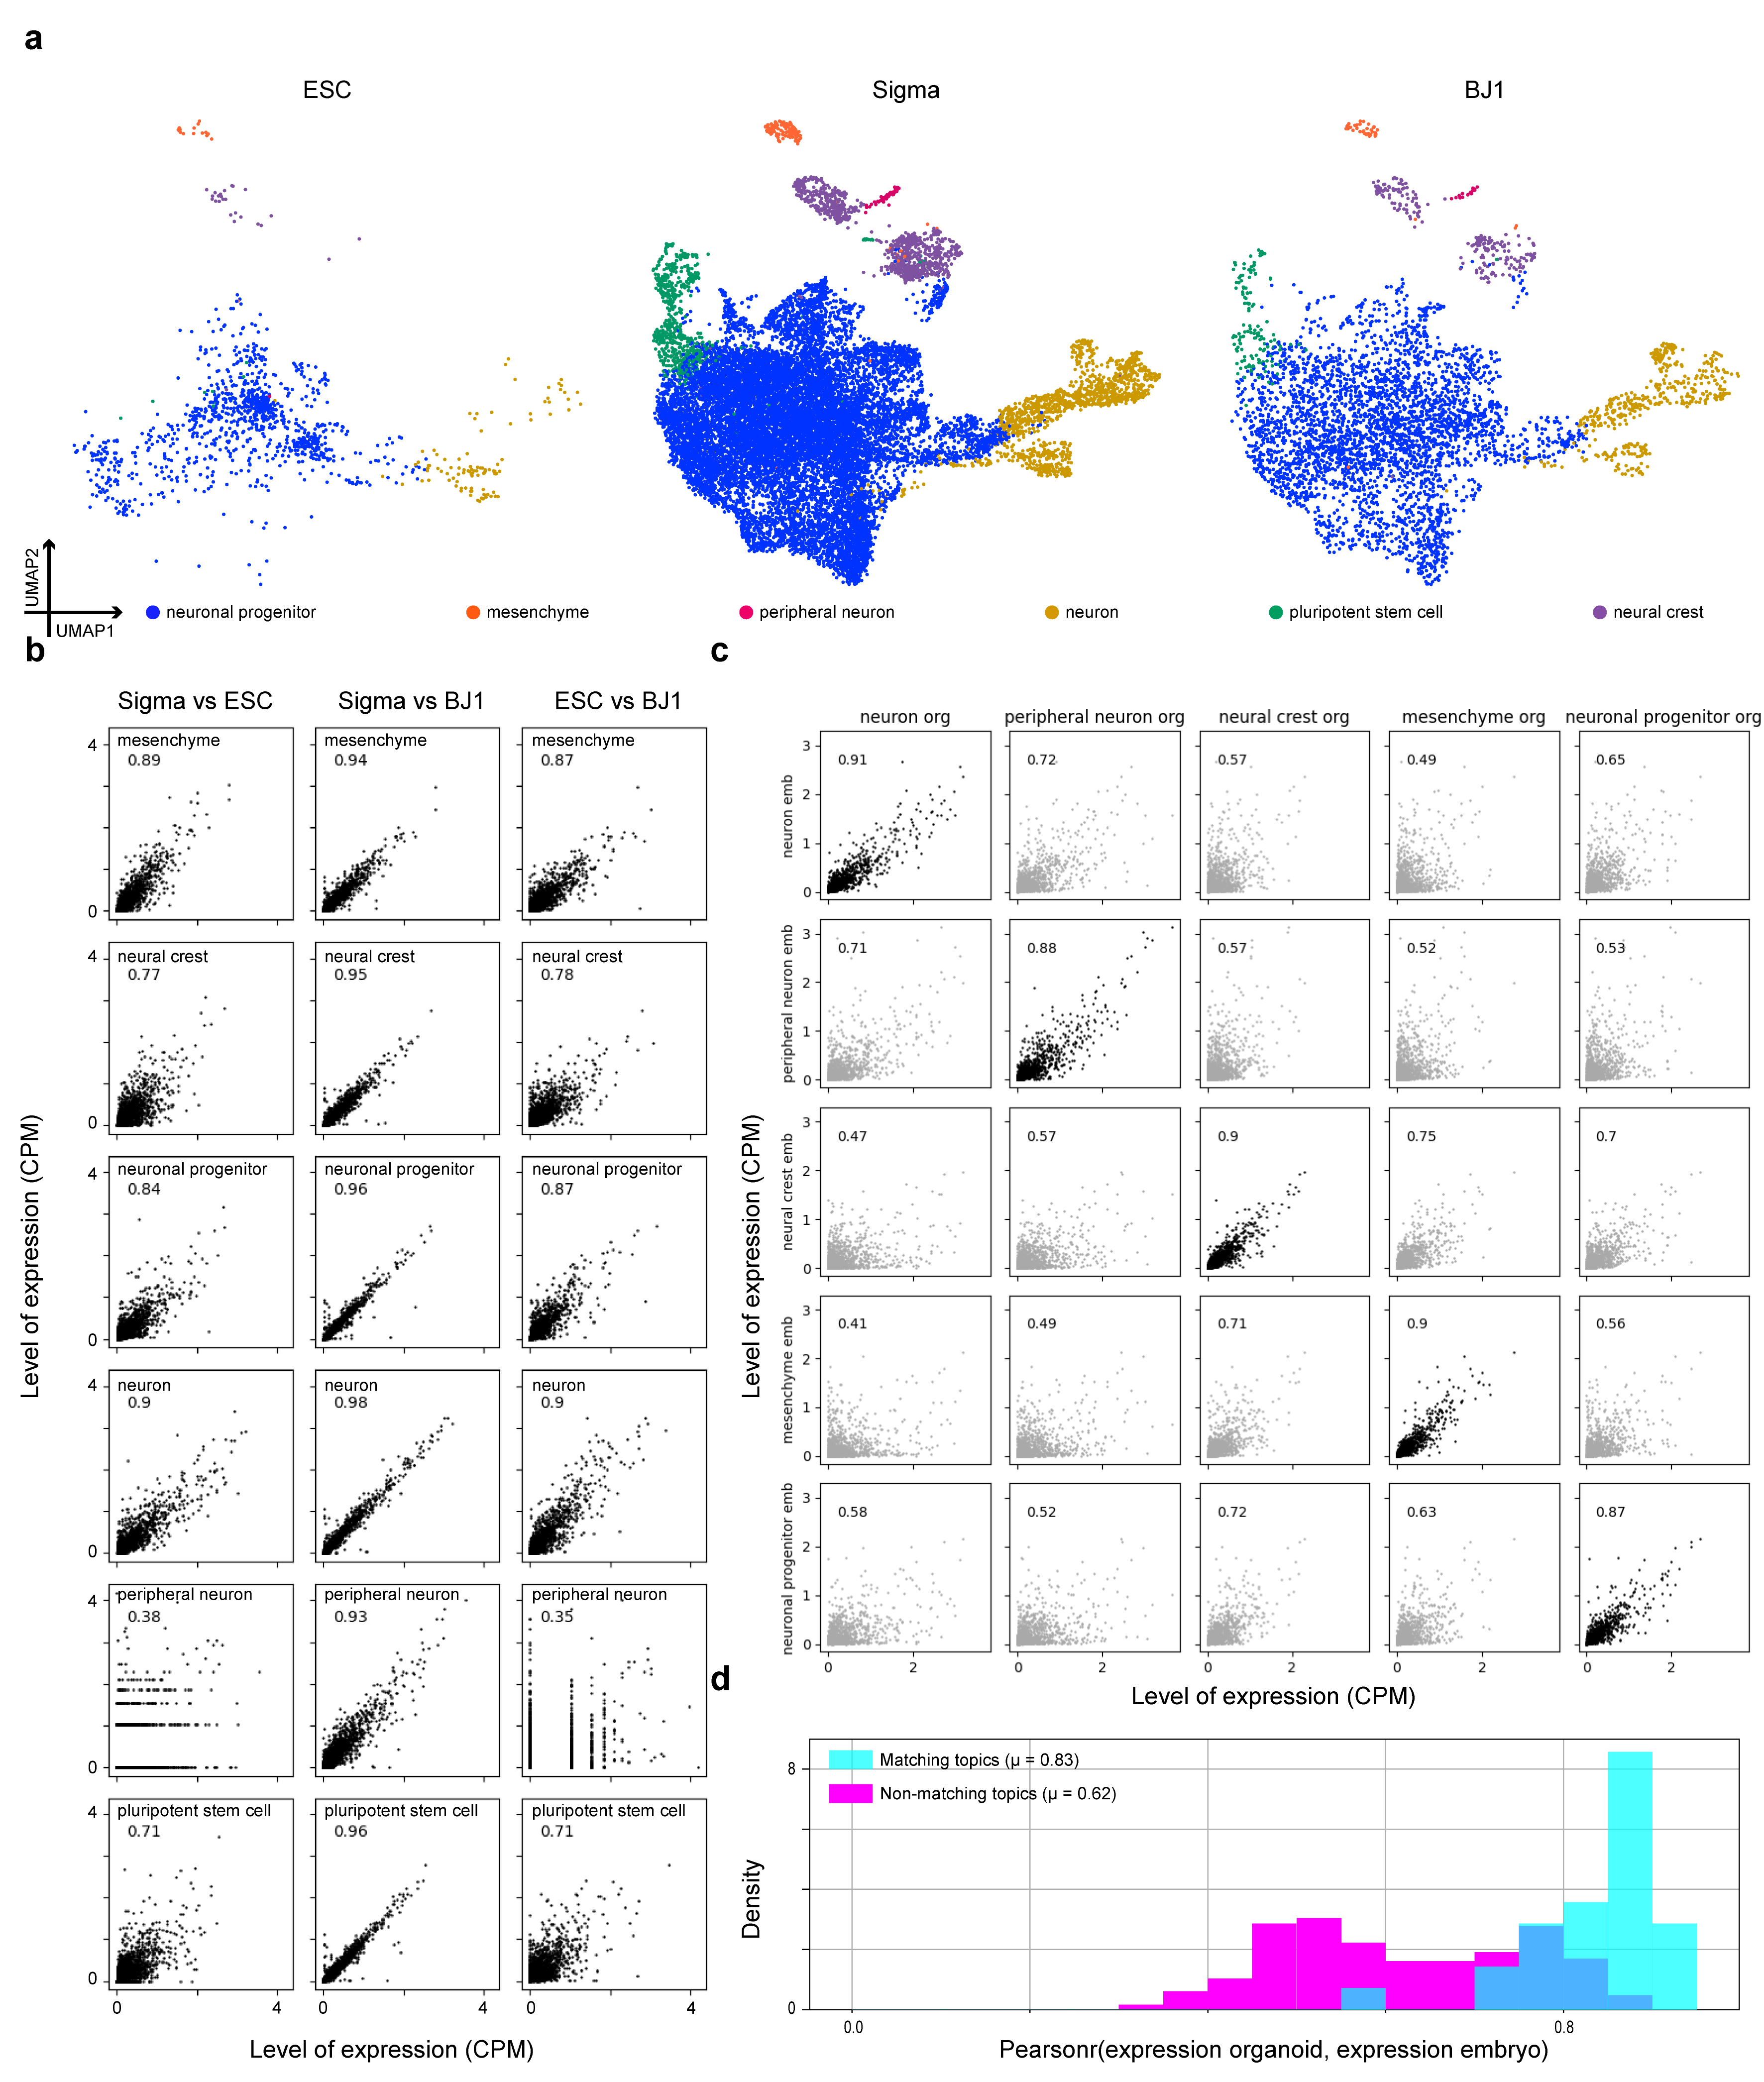
\includegraphics[width=1.0\linewidth]{figures/supplement/Supplemental_figure_1.png}
  \caption{
    \textbf{Ogranoid cell lines and embryo produce similar gene expression profiles}\\
    \textbf{a}, UMAP based on gene expression profiles of organoid cells colored by cell identity and split by cell
    line. \textbf{b}, scatter plot showing gene expression (of highly variable genes) of the same cell type across cell lines. Number top left
    indicates Pearson correlation coefficient. \textbf{c}, scatter plot showing pairwise gene expression (of highly
    variable genes) across cell types and organoid and embryo. Number top left indicates Pearson correlation
    coefficient. \textbf{d}, d histogram showing distribution of Pearson correlation coefficients of average gene
    expression profile per topic, topics representing
    the same biological state(matching) and other topics (non-matching) across organoid and embryo.
  }
\end{figure}

\newpage
\begin{figure}[p]
  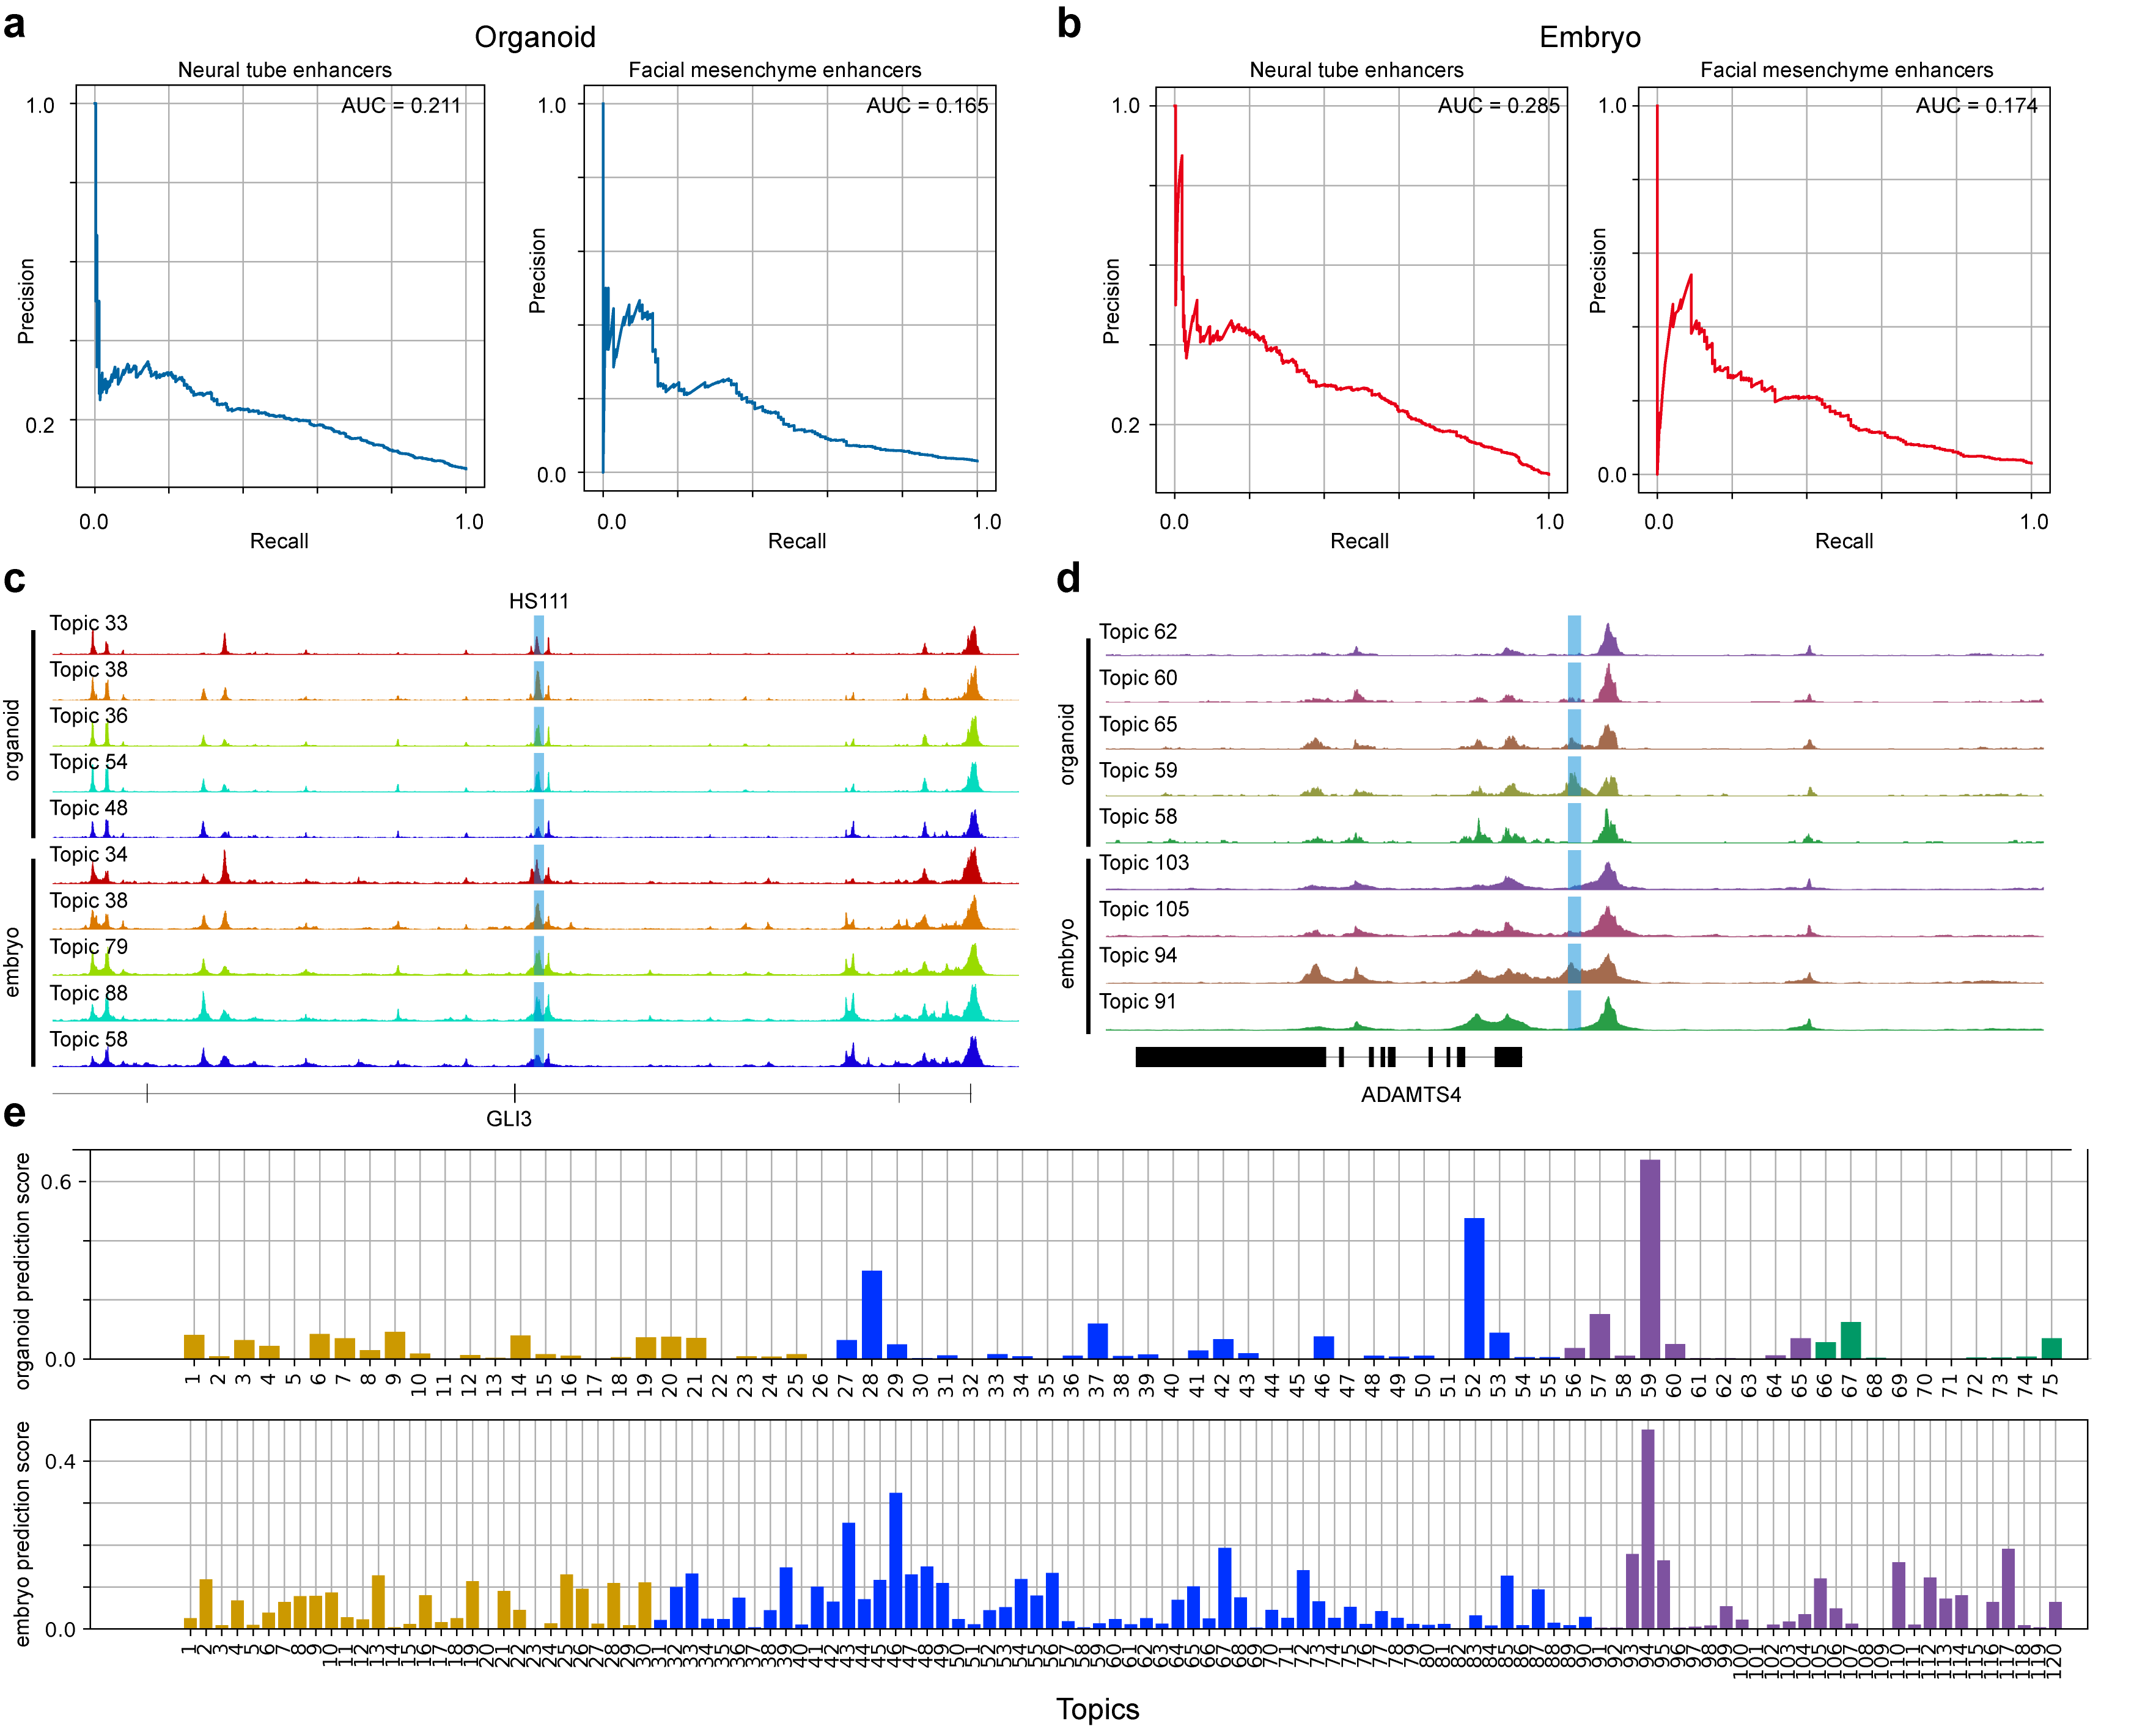
\includegraphics[width=1.0\linewidth]{figures/supplement/Supplemental_figure_2.png}
  \caption{
    \textbf{Validation of DeepNeuralTube and profiles of selected enhancers}\\
    \textbf{a-b}, precision recall curves for neural tube enhancers (left) and facial mesenchyme enhancers (right) for
    organoid (\textbf{a}) and embryo (\textbf{b}). \textbf{c}, Chromatin accessibility profile of dorso-ventral topics for organoid
    (top) and embryo (bottom) of region chr7:42,058,384-42,246,450; hg38. Location of HS111 enhancer is indicated. Values are
    CPM normalized and in range [0, 5]. \textbf{d}, Chromatin accessibility profile of neural crest topics for organoid
    (top) and embryo (bottom) of region chr1:161,183,163-161,218,934; hg38. Location of tested enhancer (chr1:161200798-161201298) is indicated.
    Values are CPM normalized and in range [0, 5]. \textbf{e}, Prediction score of $DeepNeuralTube_O$ (top) and
    $DeepNeuralTube_E$ (bottom) for each topic for neural crest enhancer chr1:161200798-161201298; hg38.
  }
\end{figure}

\newpage
\begin{figure}[p]
  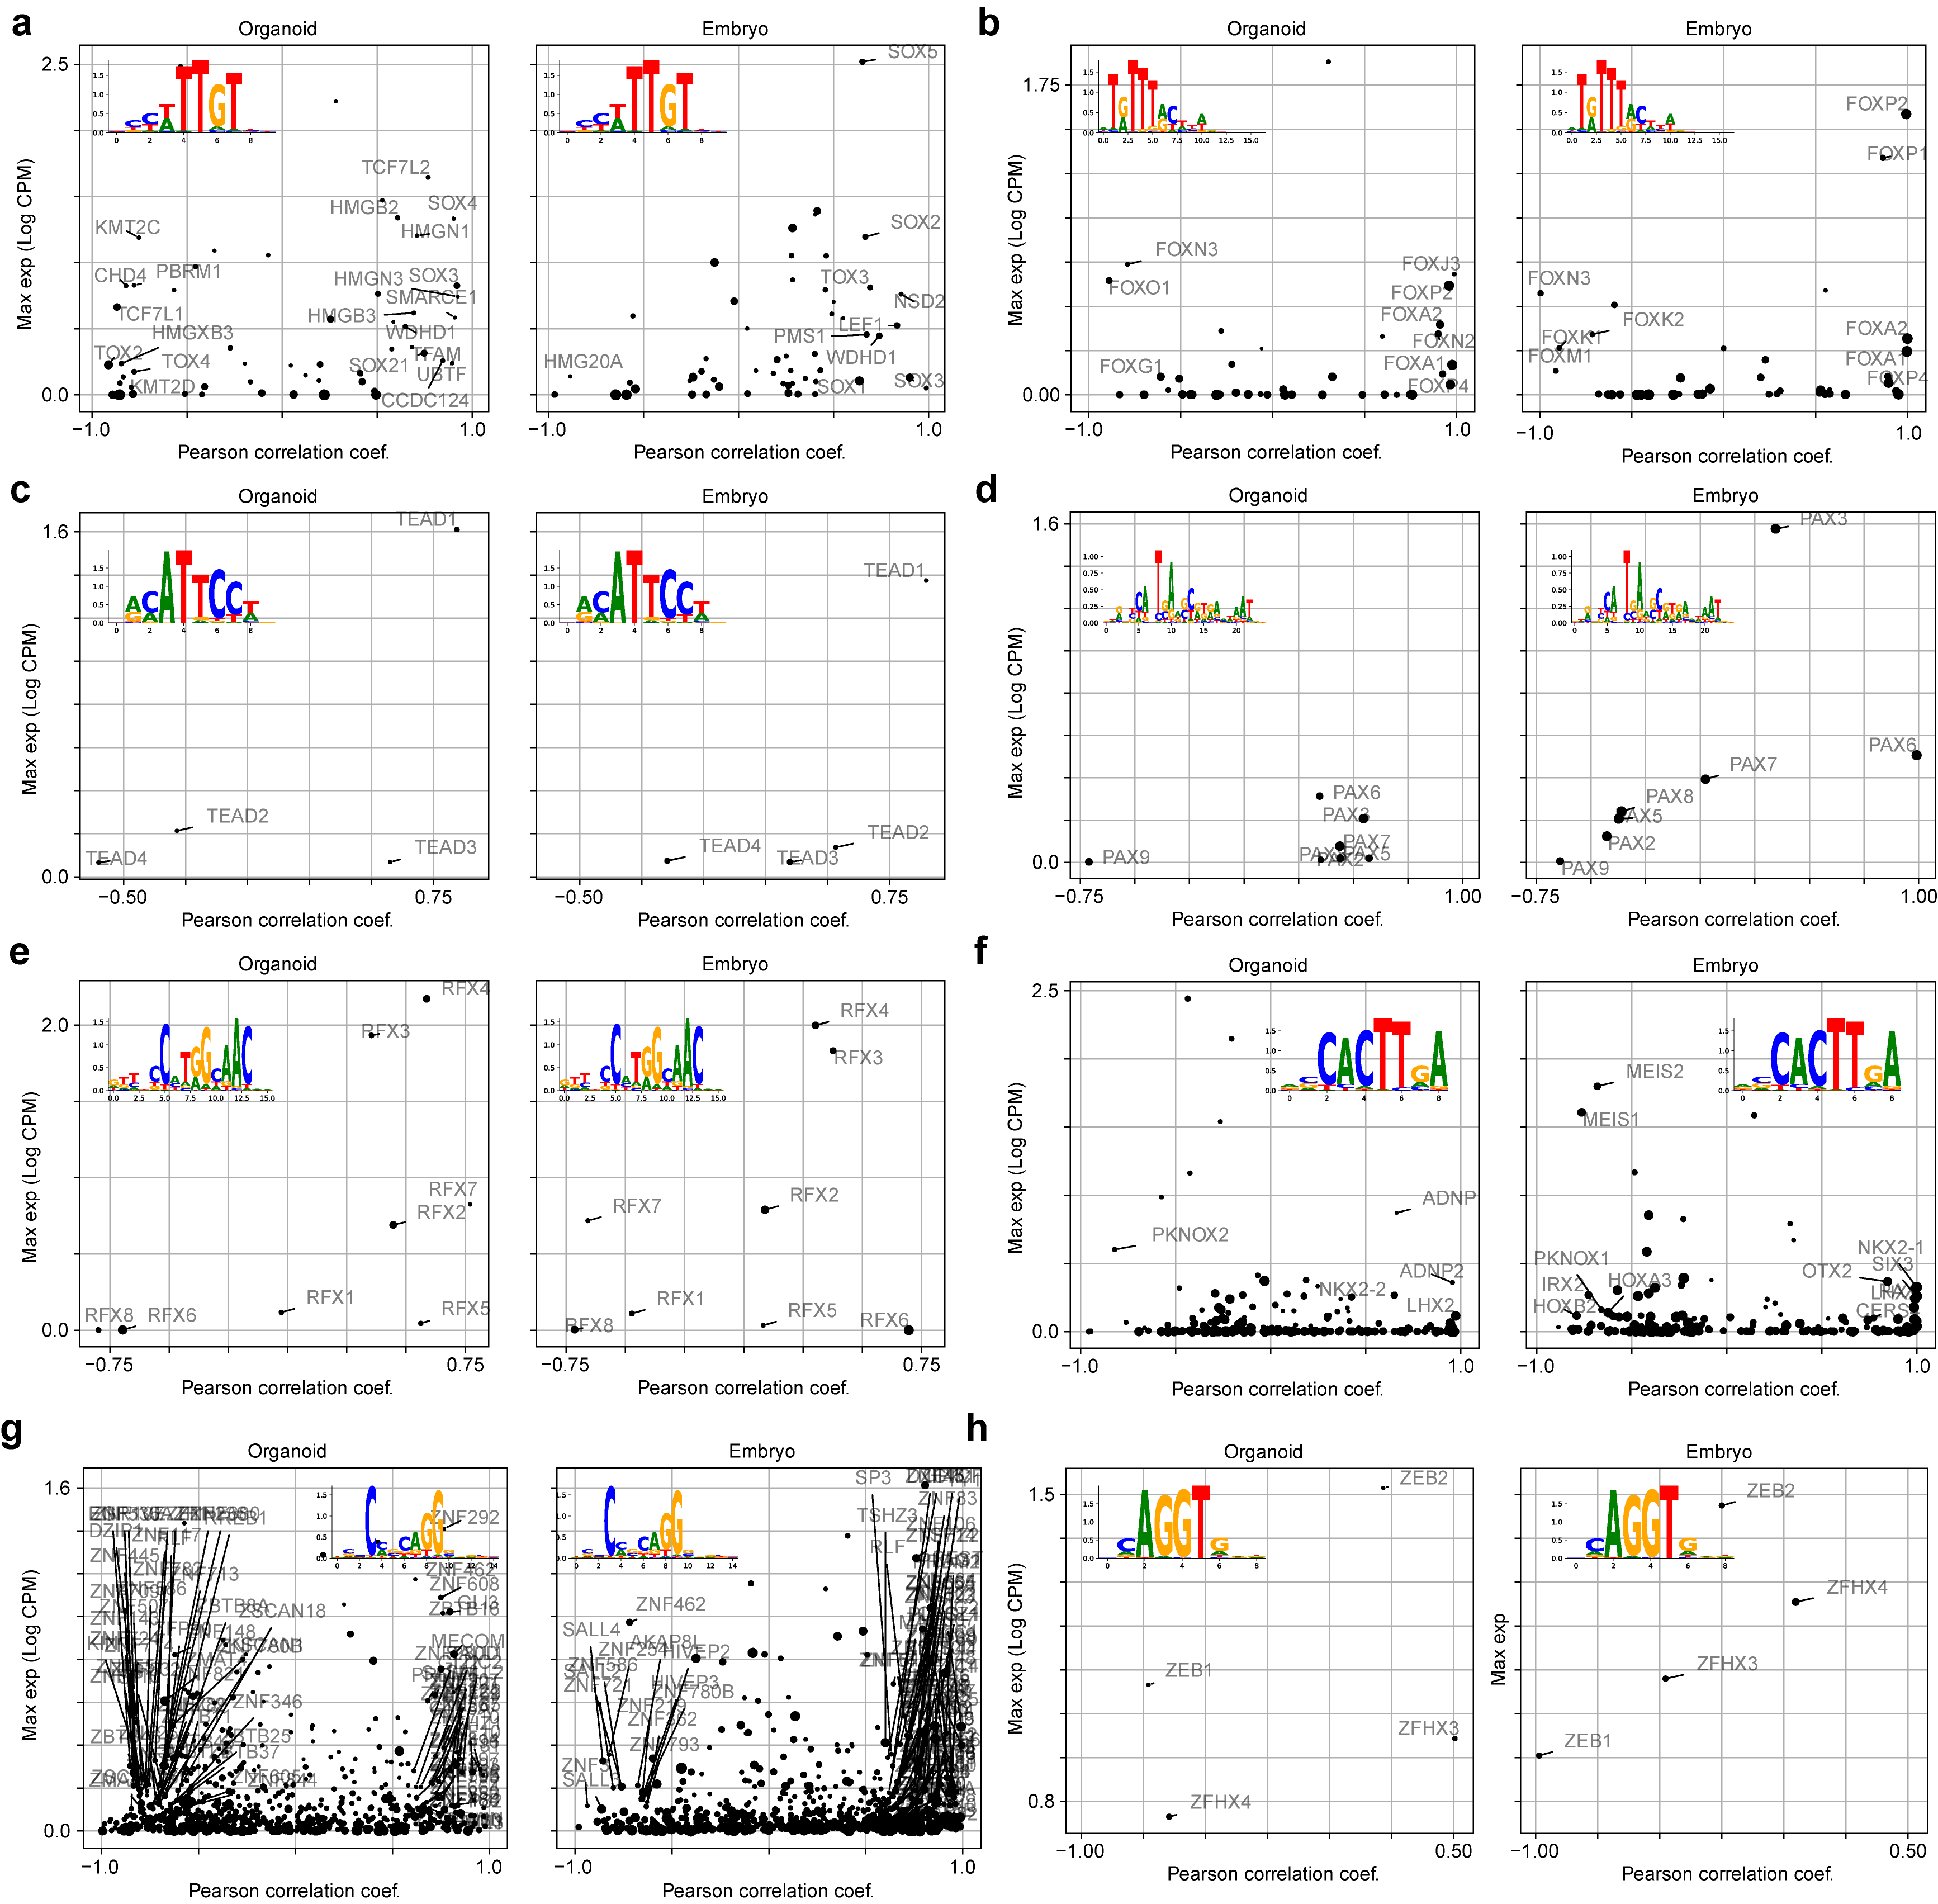
\includegraphics[width=1.0\linewidth]{figures/supplement/Supplemental_figure_3.png}
  \caption{
    \textbf{Linking motif to TF in dorso-ventral neuronal progenitors}.\\
    \textbf{a-h} Scatter plot showing Pearson correlation coefficient of average TF expression and motif importance per
    topic (x-axis) and maximum expression (Max exp; y-axis) across topics and tau index using dot size for organoid (left) and embryo (right) for TFs with DNA binding domain
    that is annotated to: HMG/Sox (\textbf{a}), Forkhead (\textbf{b}), TEA (\textbf{c}), Homeodomain; Paired box or
    Paired box (\textbf{d}), RFX (\textbf{e}), Homeodomain (\textbf{f}), C2H2 ZF (\textbf{g}) or C2H2 ZF; Homeodomain
    (\textbf{h}). Annotations according to Lambert et al.\cite{lambertHumanTranscriptionFactors2018}.
  }
\end{figure}

\newpage
\begin{figure}[p]
  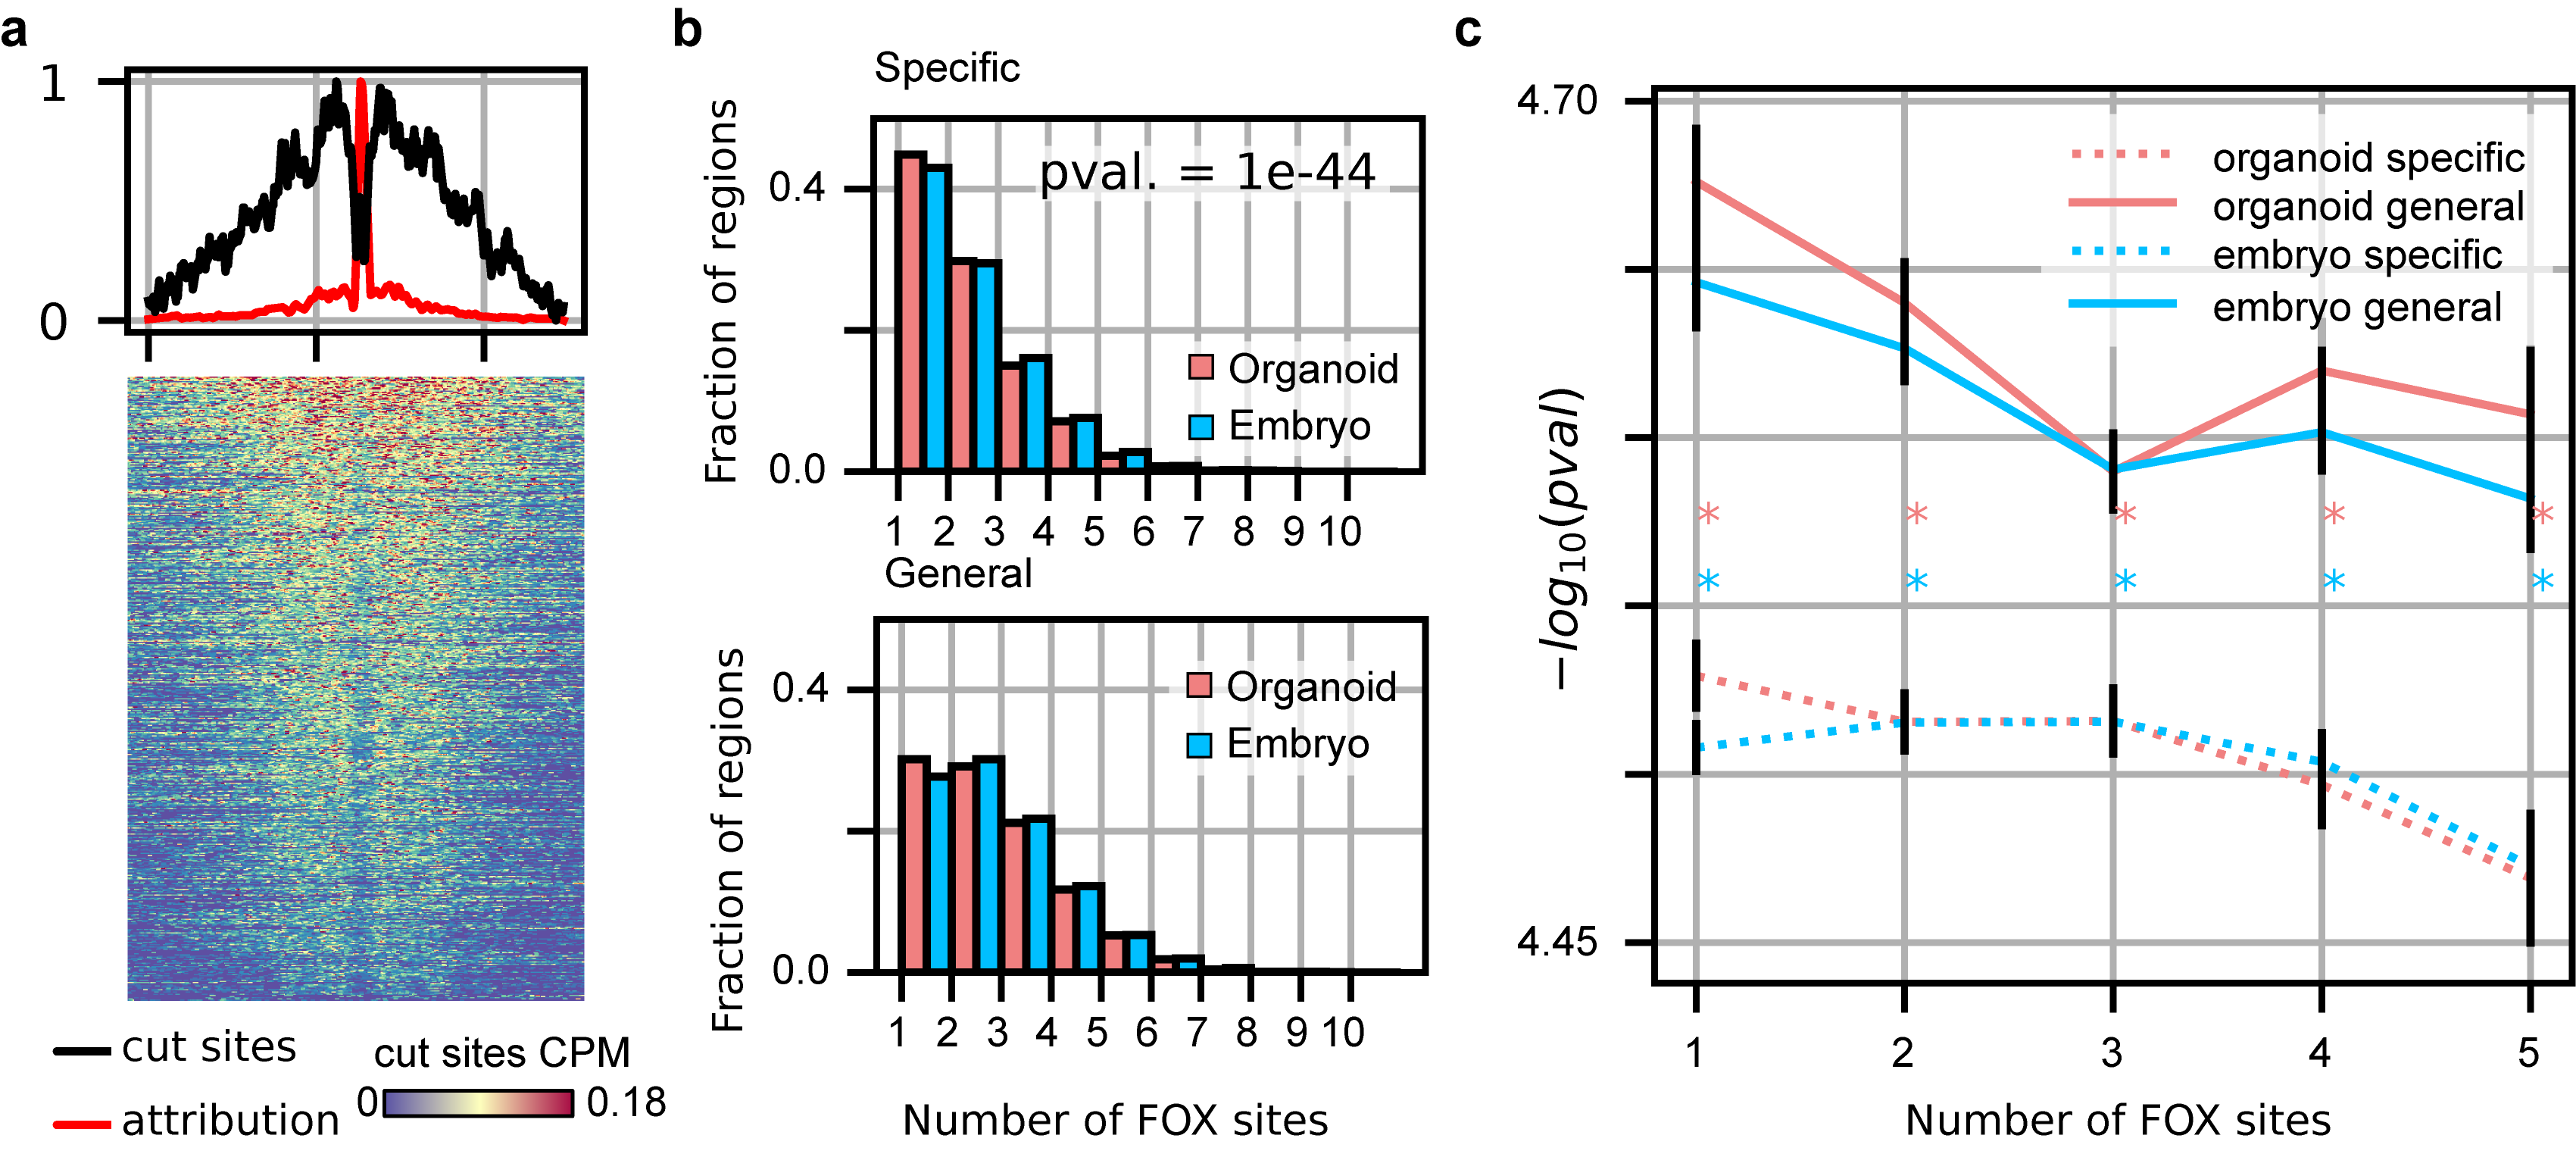
\includegraphics[width=1.0\linewidth]{figures/supplement/Supplemental_figure_4.png}
  \caption{\textbf{Linking motif to TF in anterior-posterior neuronal progenitors}.\\
    \textbf{a-e} Scatter plot showing Pearson correlation coefficient of average TF expression and motif importance per
    topic (x-axis) and maximum expression (Max exp; y-axis) across topics and tau index using dot size for organoid (left) and embryo (right) for TFs with DNA binding domain
    that is annotated to: Homeodomain or Homeodomain; Paired box or Paired box (\textbf{a-e}). Annotations according to Lambert et al.\cite{lambertHumanTranscriptionFactors2018}.
  }
\end{figure}

\newpage
\begin{figure}[p]
  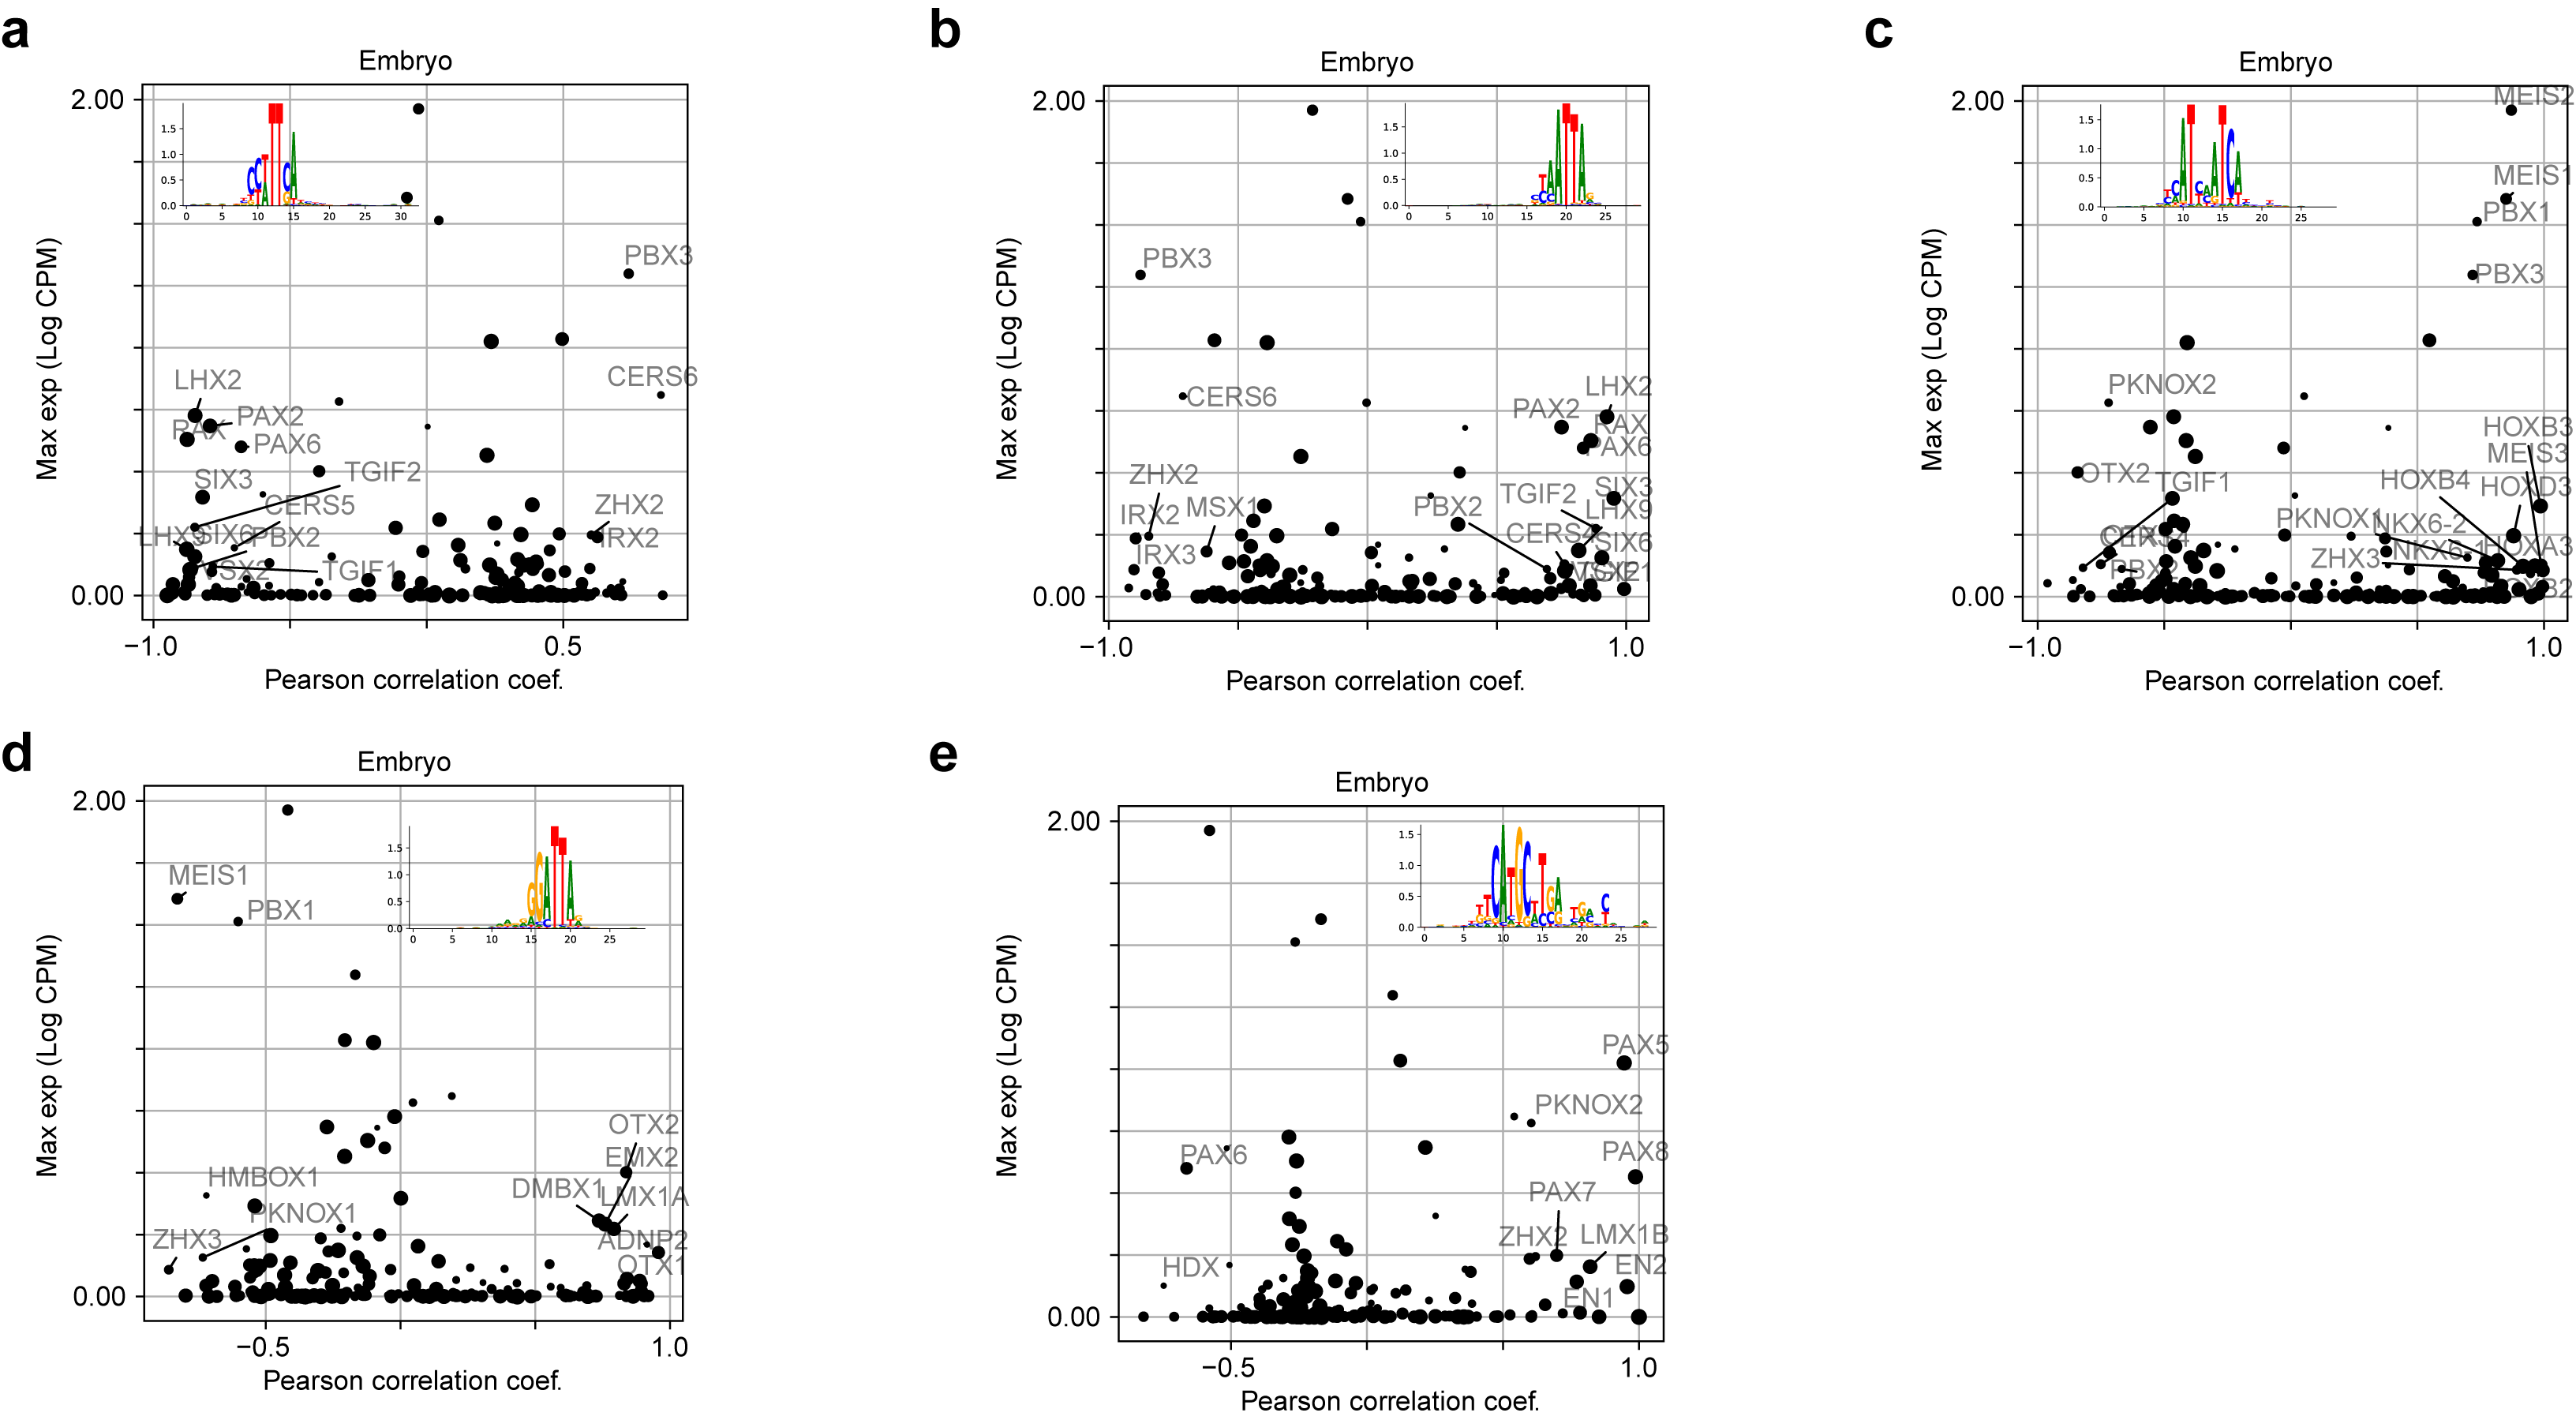
\includegraphics[width=1.0\linewidth]{figures/supplement/Supplemental_figure_5.png}
  \caption{
    \textbf{Linking motif to TF in neural crest}.\\
    \textbf{a-j} Scatter plot showing Pearson correlation coefficient of average TF expression and motif importance per
    topic (x-axis) and maximum expression (Max exp; y-axis) across topics and tau index using dot size for organoid (left) and embryo (right) for TFs with DNA binding domain
    that is annotated to:
    Forkhead (\textbf{a}), 
    HMG/SOX (\textbf{b}), 
    TEA (\textbf{c}), 
    AP-2 (\textbf{d}), 
    C2H2 ZF; Homeodomain (\textbf{e}), 
    C2H2 ZF (\textbf{f}), 
    Nuclear receptor (\textbf{g}), 
    Grainyhead (\textbf{h}), 
    bHLH (\textbf{i}), 
    RFX (\textbf{j}).
    Annotations according to Lambert et al.\cite{lambertHumanTranscriptionFactors2018}.
  }
\end{figure}
\newpage
\begin{figure}[p]
  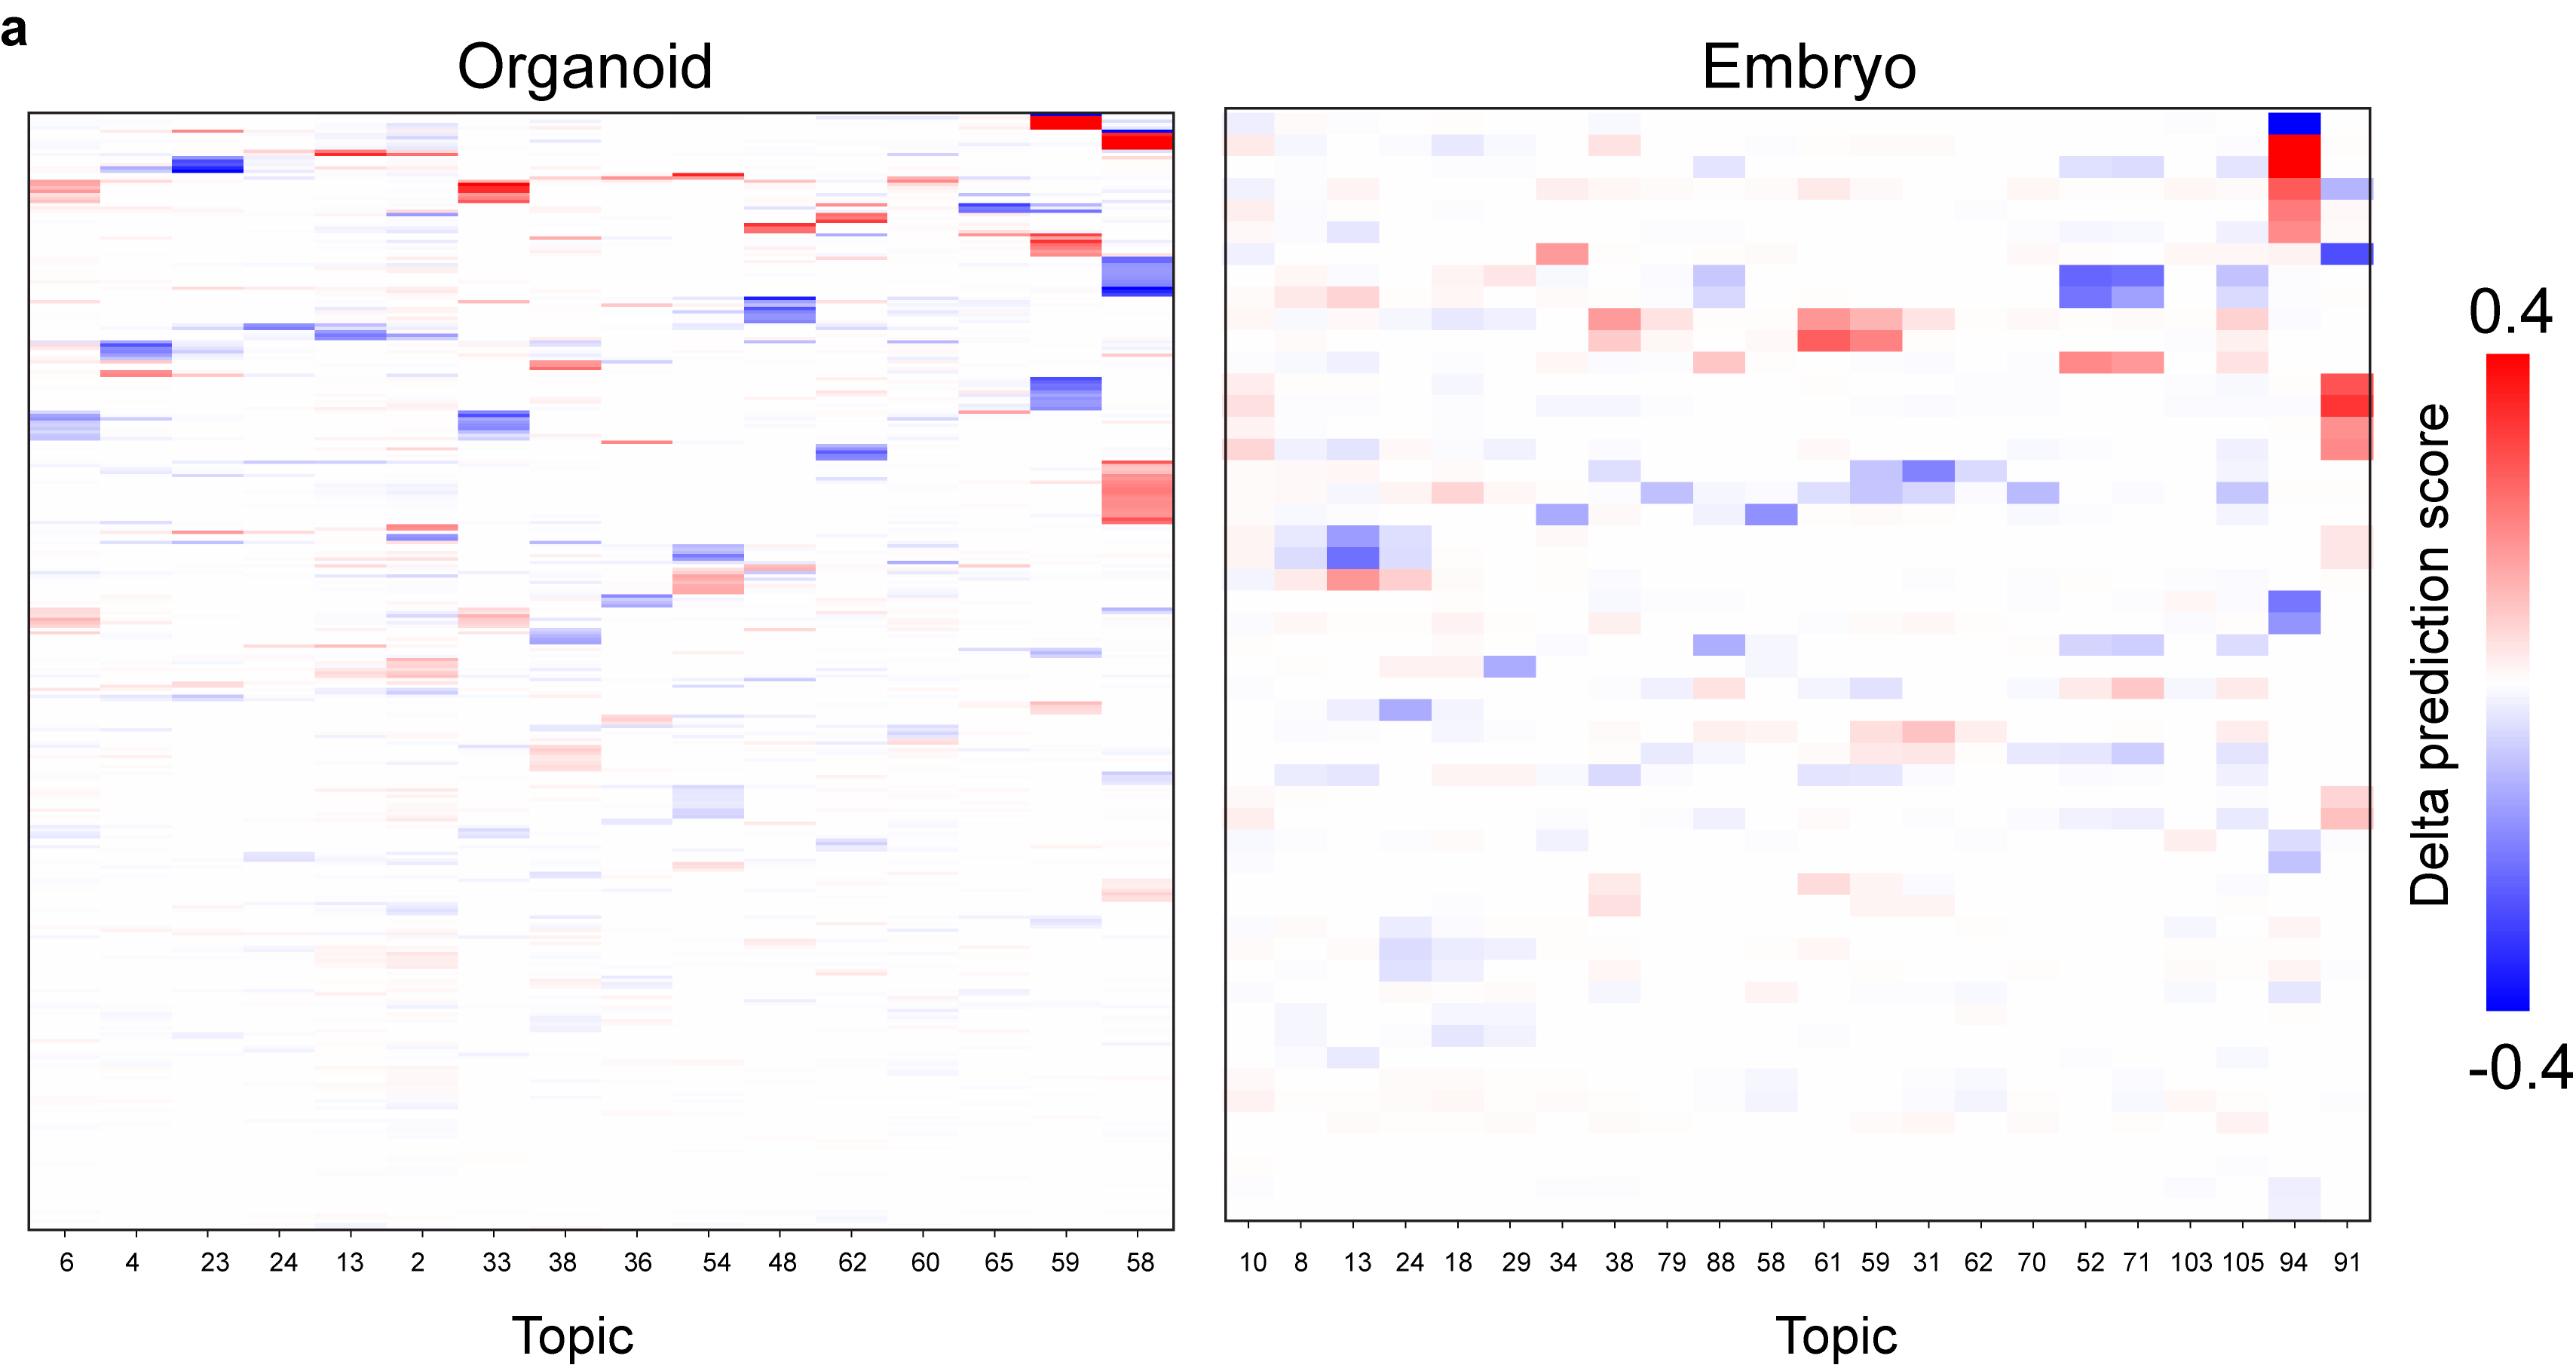
\includegraphics[width=1.0\linewidth]{figures/supplement/Supplemental_figure_6.png}
  \caption{
    \textbf{Delta prediction score across topics and SNPs}\\
    \textbf{a}, heatmap showing delta prediction score across topics using $DeepNeuralTube_O$ (left) and
    $DeepNeuralTube_E$ (right) for SNPs with a minimal absolute delta prediction score of 0.2.
  }
\end{figure}


\afterpage{\clearpage}
\newpage
\begin{figure}[p]
  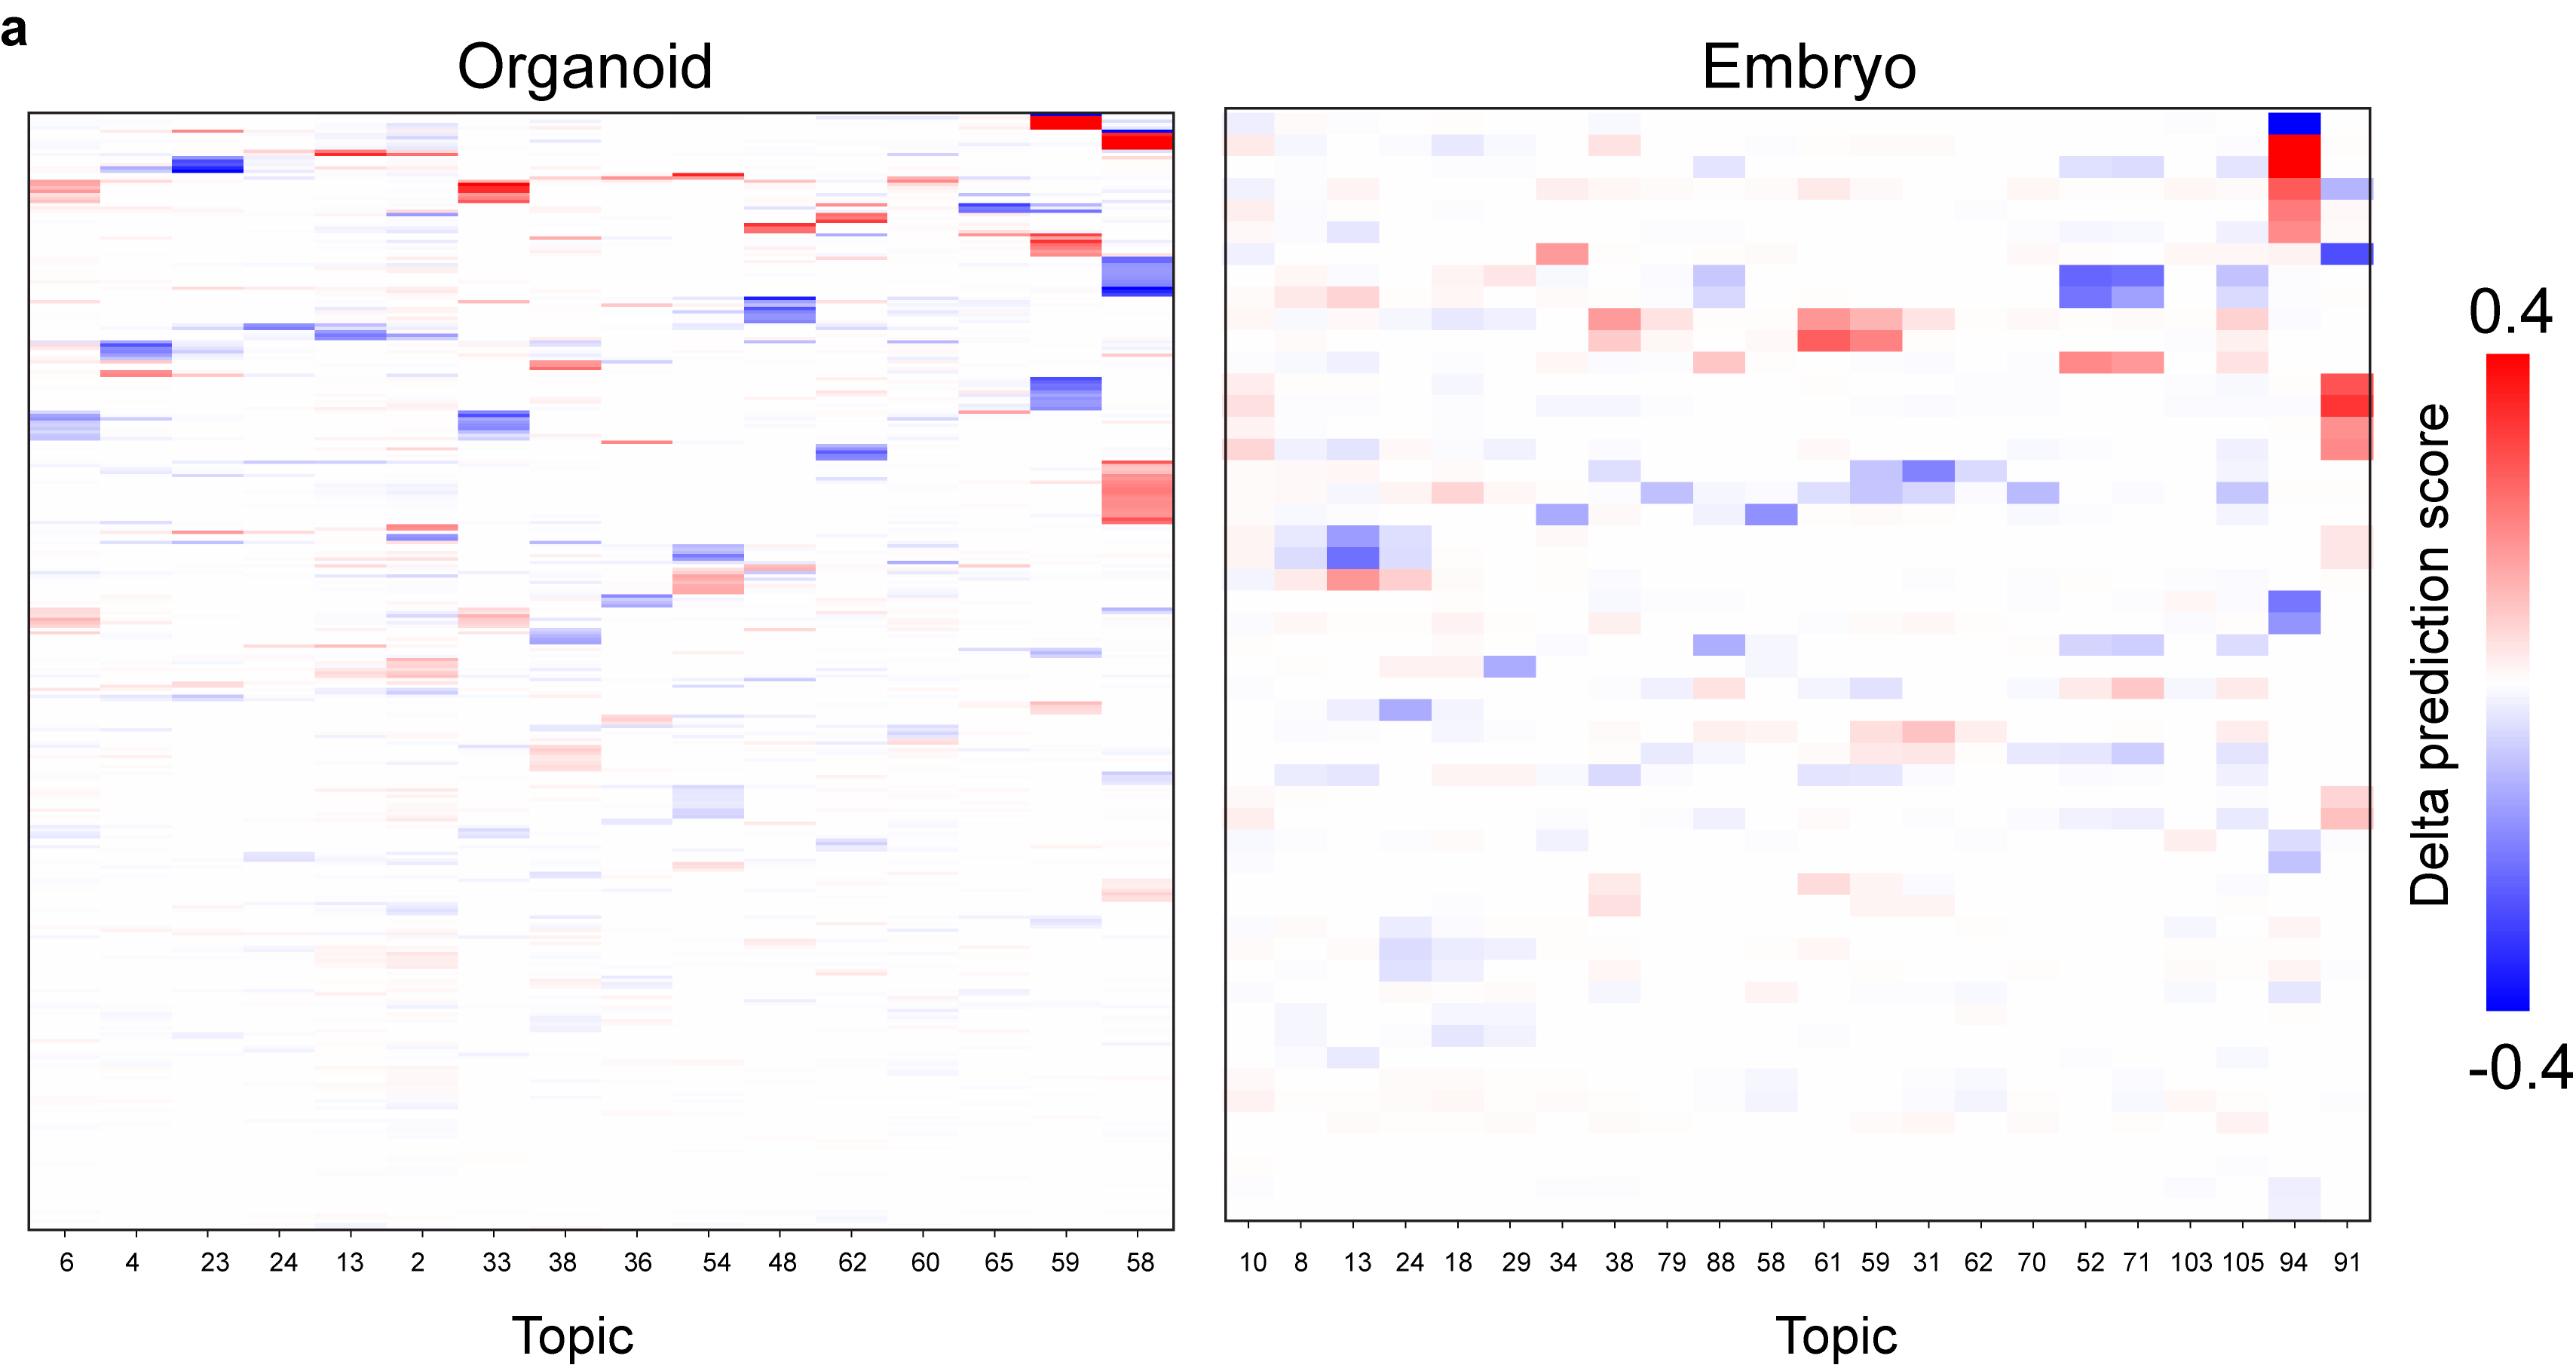
\includegraphics[width=1.0\linewidth]{figures/supplement/Supplemental_figure_7.png}
  \caption{
    \textbf{Linking motif to TF in neurons}.\\
    \textbf{a-k} Scatter plot showing Pearson correlation coefficient of average TF expression and motif importance per
    topic (x-axis) and maximum expression (Max exp; y-axis) across topics and tau index using dot size for organoid (left) and embryo (right) for TFs with DNA binding domain
    that is annotated to (Continues next page):
 }
\end{figure}
\afterpage{\clearpage}

\begin{figure}[b]
  \ContinuedFloat
  \caption*{\rule{\linewidth}{0.4pt}}
  \caption{
    (Continued)
    TEA (\textbf{a}), 
    Forkhead (\textbf{b}), 
    HMG/SOX (\textbf{c}), 
    CUT; Homeodomain (\textbf{d}), 
    Nuclear receptor (\textbf{e}), 
    C2H2 ZF; Homeodomain (\textbf{f}), 
    bHLH (\textbf{g}), 
    EBF (\textbf{h}), 
    Homeodomain (\textbf{i}), 
    GATA (\textbf{j}), 
    RFX ({\textbf{k}}).
    Annotations according to Lambert et al.\cite{lambertHumanTranscriptionFactors2018}.
  }
\end{figure}

\newpage
\begin{figure}[p]
  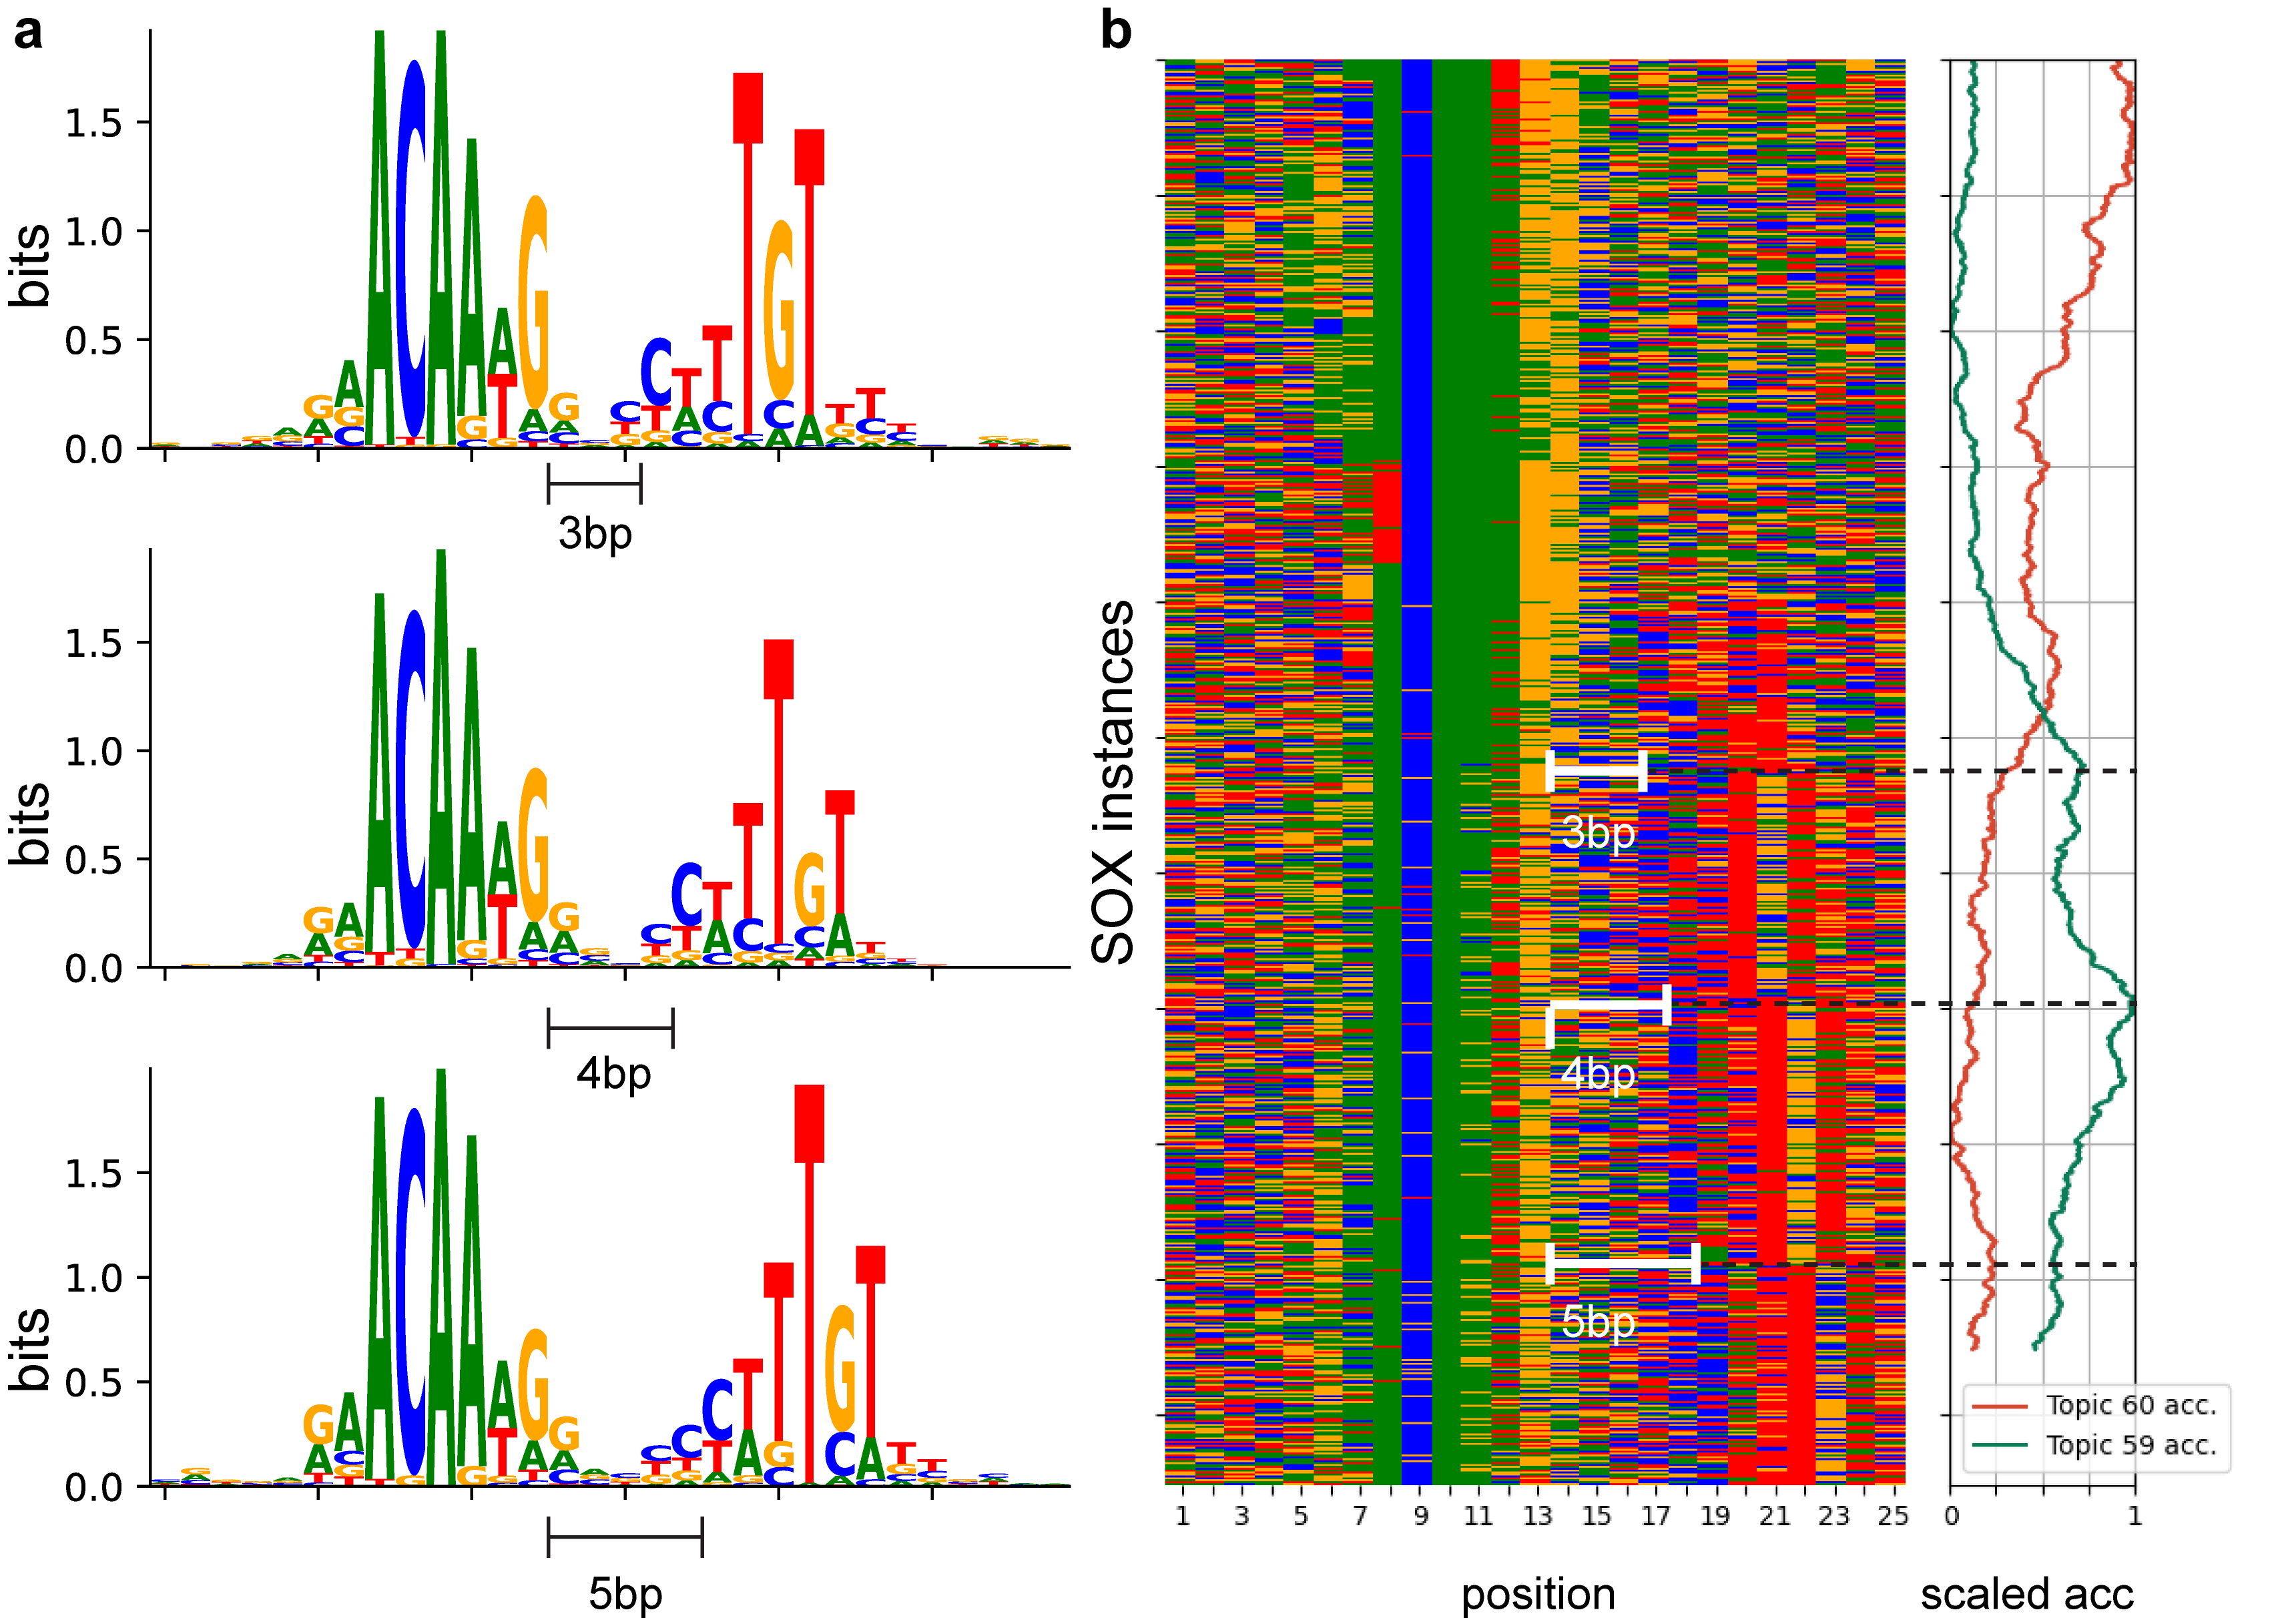
\includegraphics[width=1.0\linewidth]{figures/supplement/Supplemental_figure_8.png}
  \caption{
    \textbf{SOX dimer instances with 4bp spacing are most accessible in migratory neural crest}\\
    \textbf{a}, \textit{de novo} identified SOX dimer motifs with 3, 4, or 5 bp spacing. 
    \textbf{b}, Heatmap showing individual SOX monomer and dimer motif instances and scaled and average chromatin
    accessibility of regions with those instances for neural crest Topic 60 and Topic 59.
  }
\end{figure}

\newpage
\begin{figure}[p]
  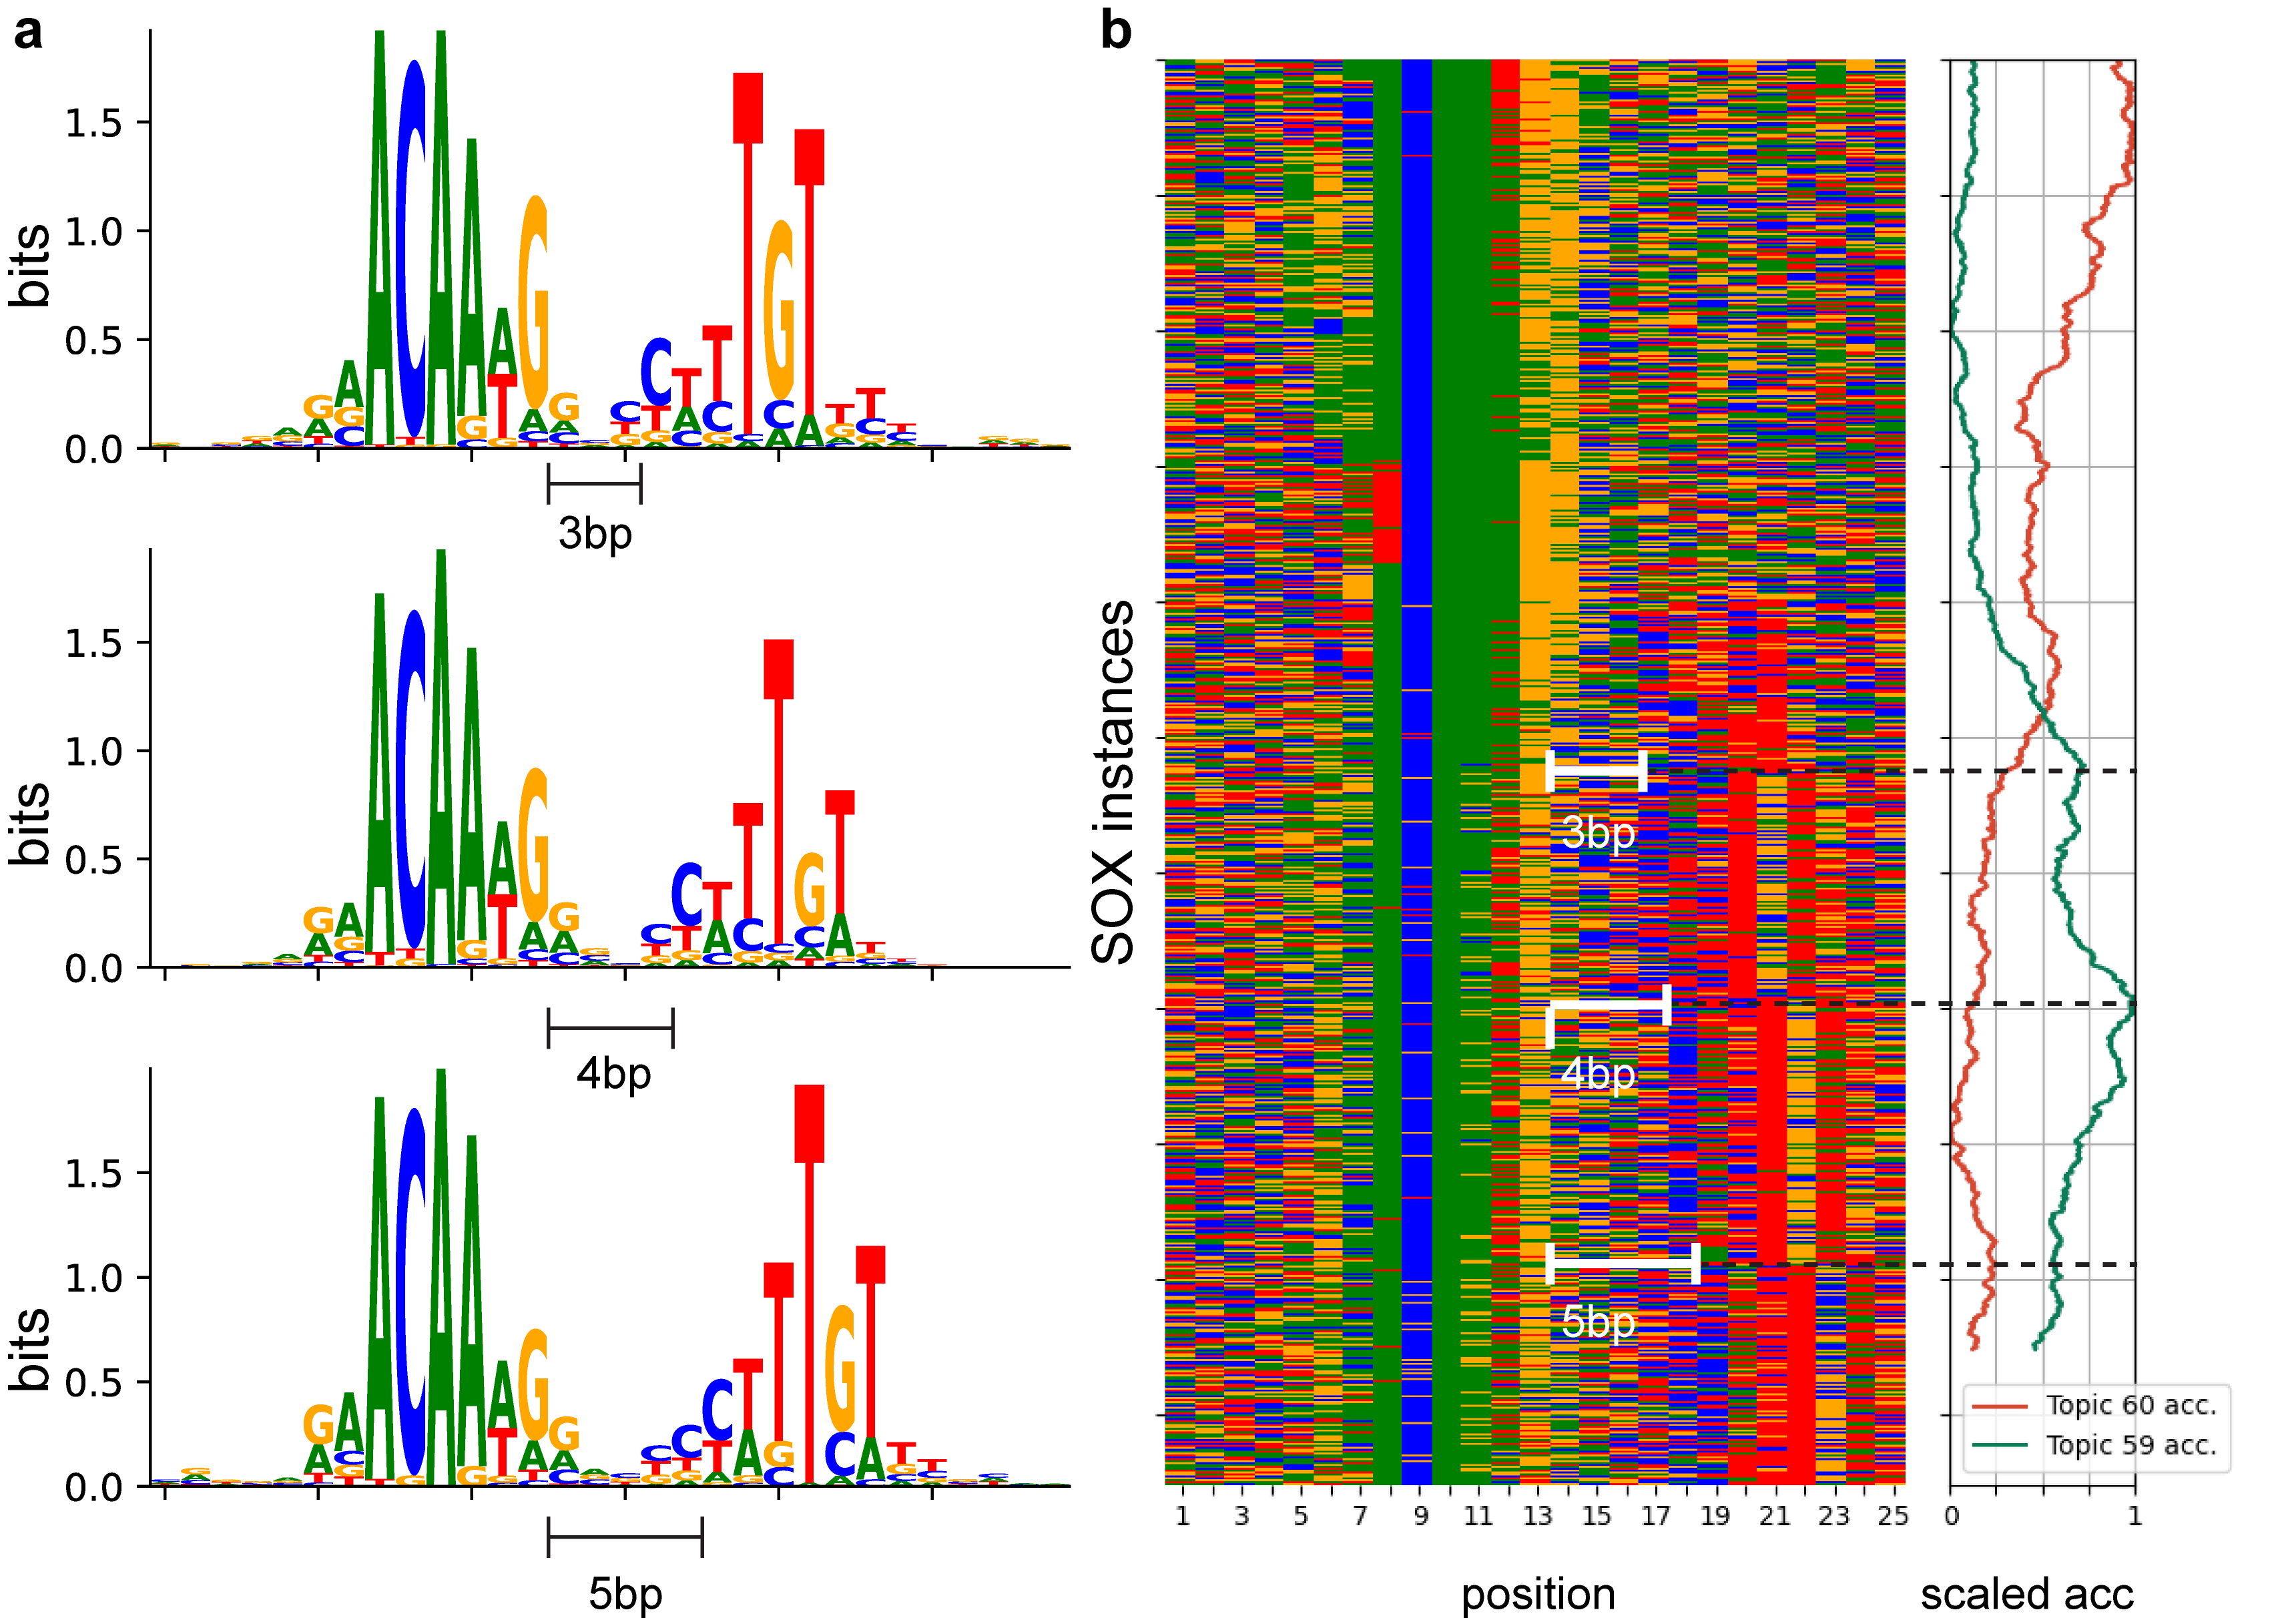
\includegraphics[width=1.0\linewidth]{figures/supplement/Supplemental_figure_9.png}
  \caption{
    \textbf{ZEB2 is a chromatin closing transcription repressor.}\\
    \textbf{a}, Network with genes (dots) and regions (outlined-dots) inferred using SCENIC+ colored by gene expression
    and chromatin accessibility in organoid pre-migratory neural crest cells. 
    \textbf{b}, scatter plot showing ZEB2 target gene expression (top) and target region accessibility (bottom) as a
    function of ZEB2 expression. Number on the top right indicates Pearson correlation coefficient.
  }
\end{figure}



\end{document}
